%\documentclass[journal]{../style/IEEE/IEEEtran}
\documentclass[11pt,a4paper]{book}
\usepackage{epsfig}
%\usepackage{graphicx}
\usepackage[dvipsnames]{color}
\DeclareGraphicsExtensions{.jpg, .eps}
\DeclareGraphicsRule{.jpg}{eps}{.jpg.bb}{`jpeg2ps -h -r 600#1}
\usepackage{amsmath,amssymb,amsthm,indentfirst,array,bbm}
\usepackage{fancyheadings}
\usepackage{longtable}

%\usepackage{wsuipa}

\usepackage[pdftex,colorlinks]{hyperref}
%\usepackage[pdftex]
%\usepackage[colorlinks]{hyperref}

\unitlength 1cm \textwidth 16cm \textheight 20.5cm \topmargin 0.0cm \oddsidemargin 0cm
\evensidemargin 0cm
\parskip 0.3cm
\setlength{\LTcapwidth}{\textwidth} % caption length for longtable

\begin{document}
%\baselineskip 0.8cm

\bibliographystyle{acm}

\def\monolix{{\sf saemix}}
\def\R{{\sf R}}

\def\chemingraphiques{fig_nb/}
%\def\cheminbiblio{}
\def\fixed_effect{\mu}
\def\covariate{c}
\def\Covariate{C}
%\def\psig{\boldsymbol{\phi}}
\def\psig{\psi}
\def\psigprime{\psig^{\prime}}
\def\psigiprime{\psig_i^{\prime}}
\def\psigk{\psig^{(k)}}
%\def\psigki{\boldsymbol{\phi_i^{(k)}}}
\def\psigki{{\psig_i^{(k)}}}
\def\psigkun{\psig^{(k+1)}}
\def\psigkuni{\psig_i^{(k+1)}}
%\def\psigi{\boldsymbol{\phi_i}}
\def\psigi{{\psig_i}}
\def\psigil{{\psig_{i,\ell}}}
\def\phig{{\phi}}
\def\phigi{{\phig_i}}
\def\phigil{{\phig_{i,\ell}}}
\def\intercept{{\fixed_effect}}
%\def\mugkun{\boldsymbol{\fixed_effect_k}}
\def\mugkun{\fixed_effect_{k+1}}
%\def\etagi{\boldsymbol{\eta_i}}
\def\etagi{{\eta_i}}
%\def\magi{\boldsymbol{A_i}}
\def\magi{{\Covariate_i}}
%\def\mgamma{\boldsymbol{\Gamma}}
%\def\mgammakun{\boldsymbol{\Gamma_k}}
\def\IIV{{\Omega}}
\def\IIVk{{\IIV_{k}}}
\def\IIVkun{{\IIV_{k+1}}}
\def\sigmakun{\sigma^2_{{k+1}}}
%\def\thetag{\boldsymbol{\theta}}
\def\thetag{{\theta}}
%\def\thetagk{\boldsymbol{\theta_k}}
\def\thetagk{{\theta_k}}
%\def\thetagkun{\boldsymbol{\theta_{k+1}}}
\def\thetagkun{{\theta_{k+1}}}
%\def\thetagkunm{\boldsymbol{\theta_{k-1}}}
\def\thetagkunm{\theta_{k-1}}
\def\sgk{s_{k}}
\def\sgkun{s_{k+1}}
%\def\yg{\boldsymbol{y}}
%\def\xg{\boldsymbol{x}}
\def\yg{y}
\def\xg{x}
\def\meanprior{{\fixed_effect_\star}}
\def\varprior{{V_\star}}
\def\thetaprior{{\theta_\star}}
\def\dprior{{d_\star}}

\def\nbeta{{n_{\fixed_effect}}}
\def\neta{{n_\eta}}
\def\ncov{M}
\def\npsi{{n_\psig}}
\def\nreg{{n_x}}
\def\npde{{\rm npde}}
\def\pde{{\rm pde}}
\def\pd{{\rm pd}}
\def\V{{\mathbf{V}}}
\def\E{{\mathbf{E}}}
\def\y{{\mathbf{y}}}
\def\true{{\sf TRUE}}
\def\false{{\sf FALSE}}

% Belhal
\newcommand{\dens}{\texttt{p}}
\def\eqs{\;}
\newcommand{\prob}{\mathbb{P}}


% raccourcis de traitement de texte
\newcommand{\h}{\hspace{0.5cm}}
\newcommand{\Prob}[1]{ \mathbb{P}\!\left(#1\right)}
\newcommand{\esp}[1]{\mathbb{E}\left(#1\right)}
\newcommand{\var}[1]{\mbox{Var}\left(#1\right)}
\newcommand{\eq}[1]{(\ref{#1})}
%
%\newcommand{\Rset}[1]{\mbox{$\mathbb{R}^{#1}$}}
\newcommand{\Rset}{\mbox{$\mathbb{R}$}}
\newcommand{\Nset}{\mbox{$\mathbb{N}$}}
\newcommand{\Lset}{\mbox{$\mathbb{L}_1(\mathbb{R})$}}
\newcommand{\Cset}[1]{\mbox{$\mathbb{C}^{#1}$}}
\newcommand{\Pset}{\mbox{$\mathbb{P}$}}
\newcommand{\Fr}{\mbox{$\mathcal{F}$}}
\newcommand{\Sr}{\mbox{$\mathcal{S}$}}
\newcommand{\Er}{\mbox{$\mathcal{E}$}}
\newcommand{\Lr}{\mbox{$\mathcal{L}$}}
\newcommand{\Yr}{\mbox{$\mathcal{Y}$}}
\newcommand{\Nr}{\mbox{$\mathcal{N}$}}
\newcommand{\Kr}{\mbox{$\mathcal{K}$}}
\newcommand{\Xr}{\mbox{$\mathcal{X}$}}
\newcommand{\limite}[2]{\mathop{\longrightarrow}\limits_{\mathrm{#1}}^{\mathrm{#2}}}
\newcommand{\pscal}[2] { \left< #1 , #2 \right> }
\newcommand{\tils} {\tilde{S}}
\newcommand{\Dt}[1]{\partial_\theta #1}
\newcommand{\DDt}[1]{\partial^2_\theta #1}
\newcommand{\Ds}[1]{\partial_s #1}
\newcommand{\htheta}{{\widehat{\theta}}}
\newcommand{\hthetaf}{{\widehat{\theta}_f}}
\newcommand{\hmu}{{\widehat{\intercept}}}
\newcommand{\hGamma}{{\widehat{\IIV}}}
\newcommand{\homega}{{\widehat{\omega}}}
\newcommand{\hthetag}{{\widehat{\theta}}}
\def\ag{a}
\def\bg{b}
\def\cg{c}
\def\Ag{A}
\def\Bg{B}
\def\Cg{C}
%\newcommand{\hthetag}{{\widehat{\theta}_{ML}}}
%\newcommand{\hthetag}{\theta_{ML}}
\newcommand{\thes}{{\theta^\star}}
\newcommand*{\ligne}[1][1]{\noindent \rule[0.4em]{\textwidth}{0.5pt}\par}
%%%%%%%%%%%%%%%%%%%%%%%%%%%%%%%%%%%%%%%%%%%%%%%%%%%%%%
%
\newtheorem{lem}{Lemma}[section]
\newtheorem{proposition}[lem]{Proposition}
\newtheorem{Rem}{Remark}
%
%\def\lignem{\noindent \line(1,0){6} \ \ {\small \monolix} \line(1,0){6} \\[0.2cm] }
\def\ligne{\noindent \line(1,0){14}}
\newcommand{\lignex}[1]{\noindent \line(1,0){7} \ \ {\small \sc Examples } \line(1,0){6} \\[0.2cm]
\begin{minipage}[t]{15cm} \texttt{\small  #1} \end{minipage} \\[0.2cm] \line(1,0){15} }
\newcommand{\lignem}[1]{\noindent \line(1,0){7} \ \ {\small \monolix } \line(1,0){6} \\[0.2cm]
\begin{minipage}[t]{15cm} {\texttt{\small  #1}} \end{minipage} \\[0.2cm] \line(1,0){15} }

\pagestyle{empty}
\begin{center}
$\phantom{  }$ 
\vskip 3cm
{\color[named]{Maroon}
{\Huge \bf \monolix} \\[.5cm]
{\Large Version 3.0} \\[.5cm]
{\sc February 2022}
\\[1cm]
}

{\color[named]{Maroon} { \Large \itshape Maintainers: Emmanuelle Comets~$^{1,2,\dag}$, Belhal Karimi~$^{3}$, \\ Maud Delattre~$^4$, Johannes Ranke~$^5$}
}

\vskip 1cm
{\color[named]{Maroon} { \Large \itshape Contributors: Audrey Lavenu~$^2$, Marc Lavielle~$^3$, 
Marilou Chanel~$^{1}$, M{\'e}lanie Guhl~$^{1,2}$,
Lucie Fayette~$^{1,2}$, Sofia Kaisaridi$^{1,2}$}
}
\vskip 3cm
\end{center}

{\color[named]{Brown}{$^1$ INSERM, IAME UMR 1137, Paris, France;  Universit\'e Paris Diderot, Paris, France}}

{\color[named]{Brown}{$^2$ University Rennes-I, Rennes, France; INSERM CIC 1414, Rennes, France}}

{\color[named]{Brown}{$^3$ INRIA, Saclay, France}}

{\color[named]{Brown}{$^4$ INRAE, Unit MaIAGE, Jouy-en-Josas, France}}

{\color[named]{Brown}{$^5$ Scientific consultant, Grenzach-Wyhlen, Germany}}

\vskip 1cm
{\color[named]{Maroon}{\bf $\dag$ Email:} emmanuelle.comets@inserm.fr}

\pagestyle{fancy}
\renewcommand{\chaptermark}[1]{
\markboth{\sc{
}\ {\sc \thechapter}.
\ #1}{}}
\renewcommand{\sectionmark}[1]{
\markright{#1}{}}

%\renewcommand{\sectionmark}[1]{\markright{#1}{}}
\renewcommand{\footrulewidth}{1pt}
\newcommand{\D}{\displaystyle} \normalsize
%\renewcommand{\sectionmark}[1]{\markboth{#1}{}}
%\renewcommand{\subsectionmark}[1]{\markright{#1}}
%\rfoot{\leftmark\\\rightmark} \lhead{\includegraphics[width=1cm]{fig_nb/logo_monolix.png}}

%\lhead{\includegraphics[width=1cm]{fig_nb/logo_monolix.png}}
%\rfoot{\sc SAEM 0.9}
%\lhead[]{\bfseries \sectionmark}
%\chead{}
%\rhead[]{\bfseries \sectionmark}
%\rhead{\leftmark}

\parskip 0.1cm
%{\scriptsize
{\small \tableofcontents }
\parskip 0.4cm

% Introduction, installation, models

\newpage

\chapter{Introduction} \label{chapter_introduction}

\monolix~is a package for the {\sf R} software~\cite{R} to perform parameter estimation in non-linear mixed effect models. It has been hosted on the CRAN since version 0.95 in June 2011.

\section{The objectives}

The objectives of \monolix~are to perform:
\begin{enumerate}
\item parameter estimation for non-linear mixed effects models
\begin{itemize}
\item[-] computing the maximum likelihood estimator of the population parameters, without any approximation of the model (linearization, quadrature approximation, \ldots), using the Stochastic Approximation Expectation Maximization (SAEM) algorithm,
\item[-] computing standard errors for the maximum likelihood estimator
\item[-] computing the conditional modes, the conditional means and the conditional standard deviations of the individual parameters, using the Hastings-Metropolis algorithm
\end{itemize}
\item goodness of fit plots
\item model selection
\begin{itemize}
\item[-] comparing several models using some information criteria (AIC, BIC)
\item[-] testing hypotheses using the Likelihood Ratio Test
\item[-] testing parameters using the Wald Test
\end{itemize}
\end{enumerate}
The R package \monolix~is an implementation of the Stochastic Approximation Expectation Maximization (SAEM) algorithm in \R~\cite{R}, developed by K\"uhn and Lavielle~\cite{Kuhn05}, and implemented in the {\sc Monolix} software available in Matlab and as a standalone software for Windows and Linux~\cite{LavielleMonolix}.

The current version of the R version of \monolix~handles only analytical functions. The following features have not yet been implemented in the R package \monolix, but are available in the {\sc Monolix} software:
\begin{itemize}
\item categorical covariates with more than 2 categories
\item models defined with differential equations
\item multi-response model
\item left censored data
\item interoccasion variability
\item prior distribution for the random effects
\item complex variables, including discrete data or repeated time to events
\item hidden Markov models
\item mixture models
\item autocorrelation of the residuals
\end{itemize}

Theoretical analysis of the algorithms used in this software can be found in \cite{Delyon, samson_jspi06, Kuhn01, Kuhn05}. Several application of SAEM in agronomy \cite{Makowski06}, animal breeding \cite{Jaffrezic06} and PKPD analysis \cite{Comets07, Lavielle07, samson_csda06, samson_sim06a, Bertrand09} have been published by several members of the {\sf Monolix} group. Several applications to PKPD analysis were also proposed during the last PAGE (Population Approach Group in Europe) meetings (\cite{page06b, page05a, page03, page04a, page06c, page05b} as well as a comparison of estimation algorithms \cite{page05c}, ({http://www.page-meeting.org}).

The present document describes the non-linear mixed effects models (section~\ref{sec:models}) and the algorithms used in this package (section~\ref{sec:methods}). The library's inputs and outputs are described in section~\ref{sec:package}. Section~\ref{sec:examples} shows some examples made available in the library (section).

\section{Installation and legalese} \label{sec:installation}

\subsection{Installation}

\subsection{Citing \monolix}

\hskip 18pt If you use this program in a scientific publication, we would like
you to cite the following reference:
\begin{quotation}
\noindent 
Comets E, Lavenu A, Lavielle M (2017). SAEMIX, an R version of the SAEM algorithm. Journal of Statistical Software, 80:1-41.
\end{quotation}

A BibTeX entry for \LaTeX$\;$ users is:

\begin{verbatim}
@Article{,
author	={Emmanuelle Comets and Audrey Lavenu and Marc Lavielle},
title	={Parameter estimation in nonlinear mixed effect models using saemix, an {R} implementation of the {SAEM} algorithm},
volume	={80},
pages	={1--41},
journal	={Journal of Statistical Software},
year	=2017	}
\end{verbatim}



\newpage

\section{The non-linear mixed effects model} \label{sec:models}

\subsection{Model for the observations} \label{sec:longitudinal}

\subsubsection{Longitudinal outcome} \label{sec:longitudinalCont}

Detailed and complete presentations of the non-linear mixed effects model can be found in \cite{Davidian95, davgil1, PinheiroBates00}. See also the many references therein.

We consider the following general non-linear mixed effects model for continuous outputs:
\begin{equation}
\label{nlme}
y_{ij}=f(x_{ij},\psigi)+ g(x_{ij},\psigi,\xi)\varepsilon_{ij} \ \ , \ 1\leq i \leq N \ \ ,
\ \ 1 \leq j \leq n_i
\end{equation}
Here,
\begin{itemize}
\item $y_{ij}\in \Rset$ is the $j$th observation of subject $i$,
\item $N$ is the number of subjects,
\item $n_i$ is the number of observations of subject $i$,
\item the regression variables, or design variables, ($x_{ij}$) are assumed to be known, $x_{ij}\in
\Rset^\nreg$,
\item for subject $i$, the vector $\psigi=(\psigil \, ; \, 1\leq \ell \leq \npsi) \in \Rset^\npsi$ is a vector of $\npsi$ individual parameters:
\begin{equation} \label{prior}
\psigi=H(\fixed_effect,\covariate_i,\etagi)
\end{equation}
where
\begin{itemize}
\item $\covariate_i =(\covariate_{im} \, ; \, 1\leq m \leq \ncov)$ is a known vector of $\ncov$ covariates,
\item $\fixed_effect$ is an unknown vector of fixed effects of size $\nbeta$,
\item $\etagi$ is an unknown vector of normally distributed random effects of size $\neta$: 
$$\etagi \sim_{i.i.d.} {\cal N}(0,\IIV)$$
\end{itemize}
\item the residual errors $(\varepsilon_{ij})$  are random variables with mean zero and variance 1,
\item the residual error model is defined by the function $g$ and some parameters $\xi$.
\end{itemize}

\subsubsection*{The residual error model} % \label{sec:residualErrorModel}
The within-group errors ($\varepsilon_{ij}$)  are  supposed  to be  Gaussian random variables  with mean  zero and variance $1$.
Furthermore, we suppose that the $\varepsilon_{ij}$ and the $\eta_{i}$ are mutually independent.

Different error models can be used in \monolix~3.0:
\begin{itemize}
\item the constant error model assumes that $g=a$ and $\xi=a$,
\item the proportional error model assumes that $g=b\,f$ and $\xi=b$,
%\item a combined error model assumes that $g=a+b\,f$ and $\xi=(a,b)$,
\item a combined error model assumes that $g=\sqrt{a^2+b^2\,f^2}$ and $\xi=(a,b)$ (note: this was changed in\monolix 3.0 from the previous model which was $g=a+b\,f$)
%\item a combined error model with power assumes that $g=a+b\,f^c$ and $\xi=(a,b,c)$,
%\item \ldots
\end{itemize}

Furthermore, all these error models can be applied to some transformation of the data:
\begin{eqnarray}\label{def_t}
t(y_{ij})=t(f(x_{ij},\psigi))+ g(x_{ij},\psigi,\xi)\varepsilon_{ij}
\end{eqnarray}

In the current version of \monolix, the exponential error model is also available: it assumes that $y>0$ and that:
\begin{eqnarray*}
t(y) &=& \log(y) \\
y&=&f e^{g\varepsilon}
\end{eqnarray*}

\subsubsection{Discrete outcome}

Categorical responses can take a finite number of possibly values, and we define the distribution $\mathcal{D}_y$ as the set of probabilities for each value, summing up to 1, so that the j$^{\rm th}$ observation $y_{ij}$ in subject $i$ follows $\mathcal{D}_y\left(x_{ij}; \psi_i, \xi \right)$. 

\paragraph{Binary data:} An example is binary response, where we model the probability of the response being 1, for exemple through the logistic model:
$$ p(y_{ij} | \psi_i) = \dfrac{e^{f(x_{ij}, \psi_i)}}{1+e^{f(x_{ij}, \psi_i)}} $$
where $f(x_{ij}, \psi_i)$ is a function of the individual parameters and the design variables. $f$ is most often a linear function, and the model is equivalently written through the logit of p, where $logit(p) = \ln \frac{p}{1-p}$, for example:
$$ logit(p(y_{ij} | \psi_i)) = \alpha_i + \beta_i x_{ij} $$

% Extending to $K$ ordered categories: $c_1 \preceq c_2 \preceq  ... \preceq c_K$, we can use models such as the continuous odds ratio to increment the cumulative probabilities:
% 
% $$\begin{cases} logit(\mathbb{P}(y_{it} \preceq c_1)) = \alpha_{i1} + \beta_i t \\
% logit(\mathbb{P}(y_{it} \preceq c_2)) = \alpha_{i1} + \alpha_{i2} + \beta_i t \\
% \vdots \\
% logit(\mathbb{P}(y_{it} \preceq c_{K-1})) = \alpha_{i1} + ... + \alpha_{iK-1} + \beta_i t \\
% \end{cases}
% \quad \text{and} \quad \begin{cases} \mathbb{P}(y_{it} = c_1) = \mathbb{P}(y_{it} \preceq c_1) \\
% \mathbb{P}(y_{it} = c_2) = \mathbb{P}(y_{it} \preceq c_2) - \mathbb{P}(y_{it} \preceq c_1) \\
% \vdots \\
% \mathbb{P}(y_{it} = c_K) = 1 - \mathbb{P}(y_{it} \preceq c_{K-1})\\
% \end{cases}
% $$

\paragraph{Categorical data:} Assume now that the observed data takes its values in a fixed and finite set of nominal categories $\{c_1, c_2,\ldots , c_K\}$. Considering the observations $(y_{ij},\, 1 \leq j \leq n_i)$ for any individual i as a sequence of conditionally independent random variables, the model is completely defined by the probability mass functions $\mathbb{P}(y_{ij}=c_k | \psi_i)$ for $k=1,\ldots, K$ and $1 \leq j \leq n_i$. For a given $(i,j)$, the sum of the K probabilities is $1$, so in fact only $K-1$ of them need to be defined. In the most general way possible, any model can be considered so long as it defines a probability distribution, i.e., for each k, $\mathbb{P}(y_{ij}=c_k | \psi_i) \in [0,1]$, and $\sum_{k=1}^{K} \mathbb{P}(y_{ij}=c_k | \psi_i) =1$. Ordinal data further assume that the categories are ordered, i.e., there exists an order $\prec$ such that

$$c_1 \prec c_2,\prec \ldots \prec c_K $$.

We can think, for instance, of levels of pain $(low \prec moderate \prec severe)$ or scores on a discrete scale, e.g., from 1 to 10. Instead of defining the probabilities of each category, it may be convenient to define the cumulative probabilities $\mathbb{P}(y_{ij} \preceq c_k | \psi_i)$ for $k=1,\ldots ,K-1$, or in the other direction: $\mathbb{P}(y_{ij} \succeq c_k | \psi_i)$ for $k=2,\ldots, K$. Any model is possible as long as it defines a probability distribution, i.e., it satisfies

$$0\leq\prob(y_{ij}\prec c_1|\psi_i)\leq\prob(y_{ij}\prec c_2|\psi_i)\leq \cdots \leq\prob(y_{ij}\prec c_K|\psi_i)=1$$


{\bf Note:} It is possible to introduce dependence between observations from the same individual by assuming that $(y_{ij},\,j=1,2,\ldots,n_i)$ forms a Markov chain. For instance, a Markov chain with memory 1 assumes that all that is required from the past to determine the distribution of $y_{ij}$ is the value of the previous observation $y_{i,j-1}$., i.e., for all $k=1,2,\ldots ,K$,

$$\prob(y_{ij}=c_k|y_{i,j-1},y_{i,j-2},y_{i,j-3},…,\psi_i)=\prob(y_{ij}=c_k|y_{i,j-1},\psi_i)$$

Such a model is currently not within the scope of \monolix.

\paragraph{Count data:} Count data can take a number of possible values, possibly infinite, and again we model the probability of each count. A common model is the Poisson model with parameter $\lambda$, where for subject $i$ at time $x_{ij}$ the probability of observing a count equal to $k$ is given by:

$$p(y_{ij} = k | \lambda_i) = \dfrac{e^{-\lambda_i(x_{ij})}}{k!}\lambda_i(x_{ij})^k $$

\subsubsection{Time-to-event outcome}

Although technically a continuous outcome, time-to-event data are modelled like discrete outcomes by considering their likelihood. In a time-to-event data model, the observations are the times at which events occur. An event may be one-off (e.g., death, hardware failure) or repeated (e.g., epileptic seizures, mechanical incidents).
To begin with, we consider a model for a one-off event. The survival function $S(t)$ gives the probability that the event happens after time $t$:
\begin{equation}\label{survival}
S(t)  \triangleq \mathbb{P}(T >t) = \exp\left\{-\int_{0}^{t}h(u)\textrm{d}u\right\}\eqs,
\end{equation}
where $h$ is called the hazard function. 
In a population approach, we consider a parametric and individual hazard function $h(\cdot,\psi_i)$.

The random variable representing the time-to-event for individual $i$ is typically written $T_i$ and may possibly be right-censored. Then, the observation $y_i$ for individual $i$ is
\begin{equation}
    y_i = \left\{
    \begin{array}{ll}
        T_i & \mbox{if } T_i \leq \tau_c \\
        "T_i > \tau_c" & \mbox{otherwise}\eqs,
    \end{array}
\right.
\end{equation}
where $\tau_c$ is the censoring time and $"T_i > \tau_c"$ is the information that the event occurred after the censoring time. 

For repeated event models, times when events occur for individual $i$ are random times $(T_{ij}, 1\leq j \leq n_i)$  for which conditional survival functions can be defined:
\begin{equation}
\mathbb{P}(T_{ij} > t|T_{i(j-1)}=t_{i(j-1)}) = \exp\left\{-\int_{t_{i(j-1)}}^{t}h(u, \psi_i)\textrm{d}u\right\}\eqs.
\end{equation}
Here, $t_{ij}$ is the observed value of the random time $T_{ij}$.
If the last event is right censored, then the last observation $y_{i,n_i}$ for individual $i$ is the information that the censoring time has been reached $"T_{i,n_i} > \tau_c"$. The conditional pdf of $y_i = (y_{ij},1\leq n_i)$ reads (see \cite{LavielleMonolix} for more details)
\begin{equation} \label{pdf_tte}
\dens(y_i |\psi_i) = \exp\left\{-\int_{0}^{\tau_c}h(u, \psi_i)\textrm{d}u \right\} \prod_{j=1}^{n_i-1} h(t_{ij},\psi_i)\eqs.
\end{equation}

\subsection{The statistical model for the individual parameters} \label{section_model_indiv}

We assume that $\psigi$ is a transformation of a Gaussian random vector $\phigi$:
\begin{equation} \label{prior2}
\psigi=h(\phigi)
\end{equation}
where, by rearranging the covariates $(\covariate_{im})$ into a matrix $\Covariate_i$, $\phigi$ can be written as:
\begin{equation} \label{prior3}
\phigi=\Covariate_i \fixed_effect + \etagi
\end{equation}

\subsubsection{Examples of transformations}
Here, different transformations $(h_\ell)$ can be used for the different components of $\psigi=(\psigil)$ where $\psigil=h_\ell(\phigil)$ for $\ell=1, 2, \ldots , \ell$.
\begin{itemize}
\item $\psigil$ has a normal distribution if $h_\ell(u)=u$
\item $\psigil$ has a log-normal distribution if $h_\ell(u)=e^u$
\item assuming that $\psigil$ takes its values in $(0,1)$, we can use a logit transformation $h_\ell(u)=1/(1+e^{-u})$, or a probit transformation $h_\ell(u)=\Prob{{\cal N}(0,1)\leq u}$.
%\item assuming that $\psigil$ takes its values in $(A,B)$, we can define $h_\ell(u)=A + (B-A)/(1+e^{-u})$, or  $h_\ell(u)=A + (B-A)\Prob{{\cal N}(0,1)\leq u}$.
\end{itemize}

In the following, we will use either the parameters $\psigi$ or the Gaussian transformed parameters $\phigi=h^{-1}(\psigi)$.

The model can address continuous and/or binary covariates. % categorical: no for the moment

\subsubsection{Example of continuous covariate model} \label{section_model_contcov}
Consider a PK model that depends on volume and clearance and consider the following covariate model for these two parameters:
\begin{eqnarray*}
CL_i & = & CL_{\rm pop}\left(\frac{W_i}{W_{\rm pop}}\right)^{\beta_{CL,W}} \left(\frac{A_i}{A_{\rm pop}}\right)^{\beta_{CL,A}} e^{\eta_{i,1}} \\
V_i & = & V_{\rm pop}\left(\frac{W_i}{W_{\rm pop}}\right)^{\beta_{V,W}}  e^{\eta_{i,2}}
\end{eqnarray*}
Where $W_i$ and $A_i$ are the weight and the age of subjet $i$ and where $W_{\rm pop}$ and $A_{\rm pop}$ are some ``typical'' values of these two covariates in the population. Here,
$\psigi$ will denote the PK parameters (clearance and volume) of subject $i$ and
$\phigi$ its log-clearance and log-volume.
Let
$$W^\star_i = \log\left(\frac{W_i}{W_{\rm pop}}\right) \quad ; \quad A^\star_i = \log\left(\frac{A_i}{A_{\rm pop}}\right) $$
Then,
\begin{eqnarray*}
\phigi &= & \left( \begin{array}{c}  \log(CL_i) \\  \log(V_i) \\ \end{array} \right) \\
&=& \left( \begin{array}{ccccc}  1 & 0 & W^\star_i & W^\star_i & 0 \\ 0 & 1 & 0 & 0 & W^\star_i \\ \end{array} \right)
\left( \begin{array}{c}  \log(CL_{\rm pop}) \\  \log(V_{\rm pop}) \\ \beta_{CL,W} \\ \beta_{CL,A} \\ \beta_{V,W} ) \\ \end{array} \right)
+  \left( \begin{array}{c}  \eta_{i,1} \\  \eta_{i,2} \\ \end{array} \right) \\
&=& \Covariate_i \fixed_effect + \etagi
\end{eqnarray*}

\subsubsection{Example of categorical covariate model} \label{section_model_catcov}
Assume that some categorical covariate  $G_i$ takes the values 1, 2, \ldots, $K$.
Assume that if patient $i$ belongs to group $k$, {\it i.e.} $G_i=k$, then
\begin{eqnarray*}
\log(CL_i) &=&  \log(CL_{{\rm pop},k}) + \eta_i
\end{eqnarray*}
where $CL_{{\rm pop},k}$ is the population clearance in group $k$.

Let $k^\star$ be the reference group. Then, for any group $k$, we will decompose the population clearance $CL_{{\rm pop},k}$ as
\begin{eqnarray*}
\log(CL_{{\rm pop},k}) = \log(CL_{{\rm pop},k^\star}) + \beta_k
\end{eqnarray*}
where $\beta_{k^\star} = 0$.

The variance of the random effects can also depend on this categorical covariate:
$$ \etagi \sim \mathcal{N}(0, \IIV_k) \ \ \ {\rm if } \ \ G_i=k $$

\noindent {\bf Remark:} It is assumed in \monolix~3.0 that the categorical covariate has only 2 categories (binary covariate). It is also assumed that the variance remains the same for both groups. Covariates with more than 2 categories can always be recoded into (N-1) binary covariates using dummy variables but this is for the moment up to the user.
%It is assumed in \monolix that the correlation matrix of the random effect is the same for all the groups. In other words, only the variances of the random effects can  differ from one group to another.

\subsection{General form of the non-linear mixed effect model (NLMEM)}

A general form of the non-linear mixed effect model regrouping the different types of responses is to define the model fully in terms of the probabilities:

$$\begin{cases} 
 y_{ij}  \sim \mathcal{D}_y\left(x_{ij}; \psi_i, \xi \right) \\ 
 \psi_i \sim \mathcal{D}_\psi \left( c_i; \fixed_effect,\IIV \right)
\end{cases}$$

The parameters of the model are $\thetag=(\fixed_effect,\IIV,\xi)$, with $\xi$ denoting the additional parameters of the residual error model for continuous response models.

We will denote $\ell(y;\theta)$ the likelihood of the observations $\yg =(y_{ij} \, ; \, 1  \leq i \leq n \ , 1
\leq j \leq n_i)$ and $p(\yg,\psig;\theta) $ the likelihood of the complete data $(\yg,\psig)= (y_{ij}, \psi_i \, ; \, 1
\leq i \leq n \ , 1 \leq j \leq n_i)$. Thus, $$\ell(y;\theta) = \int p(\yg,\psig;\theta)  \ d\psig .$$


% Methods

\newpage


\chapter{Methodology and algorithms}  \label{chapter_methodology} \label{sec:methods}

\section{Estimation of the parameters}

\subsection{The SAEM algorithm}\label{saem}

We are in a classical framework of incomplete data: the observed data is $\yg=(y_{ij} \, ; \, 1  \leq i \leq N \ , 1 \leq j \leq n_i)$, whereas the random parameters $(\psig=\psigi$ \, ; \, $1 \leq i \leq N)$ are the non observed data. Then, the complete data of the model is $(\yg,\psig)$. Our purpose is to compute the maximum likelihood estimator of the unknown set of parameters $\thetag=(\fixed_effect,\IIV,\ag,\bg,\cg)$, by maximizing the likelihood of the observations $\ell(\yg ;\theta)$.

In the case of a linear model, the estimation of the unknown parameters can be treated with the usual EM algorithm. At iteration $k$ of EM, the E-step consists in computing the conditional expectation of the complete log-likelihood $Q_k(\theta)= \esp{\log p(\yg,\psig;\theta) | \yg,\theta_{k-1} }$ and the M-step consists in computing the value $\theta_{k}$ that maximises $Q_k(\theta)$.

Following \cite{Dempster77,Wu83}, the EM sequence $(\theta_k)$ converges to a stationary point of the observed likelihood ({\it i.e} a point where the derivative of $\ell$ is 0) under general regularity conditions. In cases  where the regression function $f$ does not linearly depend on the random  effects, the E-step cannot be performed in a closed-form.

The stochastic approximation version  of the  standard EM  algorithm, proposed by \cite{Delyon} consists in replacing the usual E-step of EM by a stochastic procedure. At iteration $k$ of SAEM:
\begin{itemize}
\item {\em Simulation-step} : draw $\psigk$ from the conditional distribution  $p(\cdot|\yg;\thetagk)$.
\item {\em Stochastic approximation} : update $Q_k(\theta)$ according to
\begin{equation}
 Q_k(\theta) = Q_{k-1}(\theta) + \gamma_k ( \log p(\yg,\psigk;\theta) - Q_{k-1}(\theta) )
\end{equation}
where $(\gamma_k)$ is a decreasing sequence of positive numbers with $\gamma_1=1$. 
\item {\em Maximization-step} : update $\thetagk$ according to 
$$\thetagkun={\rm Arg}\max_{\thetag} Q_k(\theta).$$
\end{itemize}


It is shown in \cite{Delyon} that SAEM converges to a maximum (local or global) of the likelihood of the observations under very general conditions.

Here, the complete log-likelihood can be written
\begin{eqnarray*}
\log p(\yg,\psig;\theta) & = &  \log p(\yg,h(\phig);\theta) \\
&=& - \sum_{i,j}\log( g(x_{ij},\psigi,\xi) )
-\frac{1}{2} \sum_{i,j}\left( \frac{y_{ij} - f(x_{ij},\psigi)}{g(x_{ij},\psigi,\xi) } \right)^2 \\
& & -\frac{N}{2} \log (|\IIV|) -\frac{1}{2}\sum_{i=1}^{N}(\phigi-\magi\fixed_effect)^\prime \IIV^{-1}(\phigi-\magi\fixed_effect)
 -\frac{ N_{tot}+Nd}{2}\log(2\pi)
\end{eqnarray*}
where $N_{tot}=\sum_{i=1}^{N}n_i$ is the total number of observations.

First, consider a constant residual error model ($g=a$). The set of parameters to estimate is $\theta=(\fixed_effect, \IIV, \ag)$. Then, the complete model belongs to the exponential family and the approximation step reduces to only updating the sufficient statistics of the complete model:
\begin{eqnarray*}
s_{1,i,k} &= & s_{1,i,k-1}  + \gamma_k \left(  \phig_{i,k} - s_{1,i,k-1}   \right) , \hspace{1em}i=1,\ldots,N \\
 s_{2,k} &= & s_{2,k-1}  + \gamma_k \left( \sum_{i=1}^{N} \phig_{i,k} \, \phig_{i,k}^\prime - s_{2,k-1}   \right)  \\
 s_{3,k} &= & s_{3,k-1}  + \gamma_k \left( \sum_{i,j} \left( y_{ij} - f(x_{ij},\psigki) \right) ^2      - s_{3,k-1} \right) .
% s_{3,k} &= & s_{3,k-1}  + \gamma_k \left( S_{3,k-1}   - s_{3,k-1} \right) .
\end{eqnarray*}
Then, $\theta_{k+1}$ is obtained in the maximization step as follows:
 \begin{eqnarray}
\mugkun &= &\left( \sum_{i=1}^{N}  \magi^\prime \IIVk ^{-1} \magi\right)^{-1} \sum_{i=1}^N \magi^\prime \IIVk ^{-1} s_{1,i,k}  \\
\IIVkun &=& \frac{1}{N} \left(s_{2,k}- \sum_{i=1}^N(\magi\mugkun)s_{1,i,k}^\prime -\sum_{i=1}^N s_{1,i,k}(\magi\mugkun)^\prime +\sum_{i=1}^N (\magi\mugkun)(\magi\mugkun)^\prime\right) \label{react_gamma} \\
\ag_{k+1} & = & \sqrt{ \frac{s_{3,k}}{N_{tot}} }
\end{eqnarray}


\noindent {\bf Remark 1:  } The sequence of step sizes used in \monolix~decreases as $k^{-a}$. More precisely, for any sequence of integers $K_1,K_2,\ldots,K_J$ and any sequence $a_1,a_2,\ldots,a_J$ of real numbers such that $0\leq a_1 <a_2<\ldots<a_J\leq 1$, we define the sequence of step sizes $(\gamma_k)$ as follows:
\begin{equation} \label{stepsize1}
\gamma_k = \frac{1}{k^{a_1}} \quad \mbox{for any } 1\leq k \leq K_1
\end{equation}
and for $2\leq j \leq J$,
\begin{equation} \label{stepsize2}
\gamma_k = \frac{1}{\left(k - K_{j-1}+\gamma_{K_{j-1}}^{-1/a_j}\right) ^{a_j}} \quad \mbox{for any } \sum_{i=1}^{j-1} K_i +1\leq k \leq \sum_{i=1}^{j} K_i
\end{equation}
Here, $K=\sum_{j=1}^{J}K_j$ is the total number of iterations.

We recommend to use $a_1=0$ (that is $\gamma_k=1$) during the first iterations, and $a_J=1$ during the last iterations. Indeed, the initial guess  $\theta_0$ may  be far  from the maximum likelihood value  we are looking for and the first iterations with $\gamma_k=1$ allow to converge quickly to a neighborhood of the maximum likelihood estimator. Then, smaller step sizes ensure the almost sure convergence of the algorithm to the maximum likelihood estimator.


\frame{\parbox{15cm} {\vspace*{.2cm} \quad In the case where $J=2$ with $a_1=0$ and $a_2=1$, the sequence of step sizes  is
\begin{eqnarray*}
\gamma_k &=& 1  \quad  \quad \quad \quad  \mbox{ for } 1\leq k \leq K_1 \\
 &=& \frac{1}{k-K_1+1}  \quad \mbox{ for } K_1+1 \leq  k \leq K_1+K_2
\end{eqnarray*}
}}


\noindent {\bf Remark 2:  } The estimated covariance matrix $\IIVkun$ defined in (\ref{react_gamma}) is a full covariance matrix. However, the covariance matrix $\IIV$ of the random effects can have any covariance structure. If we assume, for example, that there is no correlation between the random effects, we will set to 0 the non diagonal elements of $\IIVkun$ defined in (\ref{react_gamma}).

We can also assume that a random effect has no variance. If the $\ell$th random effect has a variance equal to 0, then the $\ell$th individual parameter is no longer random and the simulation step of SAEM needs some modification. During the first $K_0$ iterations, we use SAEM as it was described above, considering that all the effects are random and assuming that there is no correlation between the $\ell$th random effect and the other ones ($\omega^2_{\ell \ell^\prime}=0$ for any $\ell \neq \ell^\prime$). Then, during the next iterations, we use again SAEM, but the variance of this random effect is no longer estimated: it is forced to decrease at each iteration by setting
\begin{equation}
\omega^2_{\ell\ell,k+1}= \alpha \ {\omega^2_{\ell\ell,k}} \quad , \quad K_0 \leq k \leq K
\end{equation}
where $\alpha$ is chosen between 0 and 1 such that $\omega^2_{\ell\ell,K}= 10^{-6}\omega^2_{\ell\ell,K_0}$.

\noindent {\bf Remark 3:} - For a  residual variance model of the form $g=  \bg \, f^\cg$, where $\cg$ is fixed, the complete model also belongs to the exponential family and the estimation of $\bg$ is straightforward:  the sufficient statistics sequence $(s_{3,k})$ is defined by
$$ s_{3,k} =  s_{3,k-1}  + \gamma_k \left(
\sum_{i,j} \left( \frac{y_{ij} - f(x_{ij},\psigki)}{f^\cg (x_{ij},\psigki)}  \right) ^2  - s_{3,k-1}
\right) $$ and $\bg_{k+1} =  \sqrt{ s_{3,k}/ N_{tot} }$.

- For a general residual variance model $g= \ag + \bg \, f^\cg$, the complete model does not belong to the exponential family and the estimates of the residual variance parameters $(\ag,\bg,\cg)$ cannot be expressed as a function of some sufficient statistics. Then, let $(\Ag_k,\Bg_k,\Cg_k)$ that minimise the complete log-likelihood:
$$(A_k, B_k,C_k) = {\rm Arg}\min_{(\ag,\bg,\cg)}
\left\{ \sum_{i,j}\log( \ag + \bg f^{\cg}(x_{ij},\psigki) ) +\frac{1}{2} \sum_{i,j}\left(
\frac{y_{ij} - f(x_{ij},\psigki)}{\ag + \bg f^{\cg}(x_{ij},\psigki) } \right)^2 \right\}
$$
We update the residual variance parameters as follows:
 \begin{eqnarray}
\ag_{k+1} & = & \ag_{k} +  \gamma_k \left(  A_k - \ag_{k}  \right)   \\
\bg_{k+1} & = & \bg_{k} +  \gamma_k \left(  B_k - \bg_{k}  \right)   \\
\cg_{k+1} & = & \cg_{k} +  \gamma_k \left(  C_k - \cg_{k}  \right)
\end{eqnarray}
The estimation of $\fixed_effect$ and $\IIV$ remains unchanged.


\subsection{The MCMC-SAEM algorithm}
For model (1.1), the simulation step cannot be directly performed. Kuhn and Lavielle \cite{Kuhn01} propose to combine the SAEM algorithm with a MCMC (Markov Chain Monte Carlo) procedure. This procedure consists in replacing the Simulation-step at iteration $k$ by $m$ iterations of the Hastings-Metropolis algorithm.

Here, we will consider the Gaussian parameters $(\phigi)$. For $i=1,2,\ldots,N$
\begin{itemize}
\item let $\phig_{i,0}=\phig_{i}^{(k-1)}$
\item for $p=1,2,\ldots,m$,
\begin{enumerate}
\item draw $ \tilde{\phig}_{i,p}$ using the proposal kernel
$ q_{\theta_k}( \phig_{i,p-1} ,\cdot) $
\item set $ \phig_{i,p} =  \tilde{\phig}_{i,p} $ with probability
$$ \alpha( \phig_{i,p-1} ,  \tilde{\phig}_{i,p} ) = \min \left(1, \frac
{ p( \tilde{\phig}_{i,p} |y_i;\theta_k) q_{\theta_k}(\tilde{\phig}_{i,p} , \phig_{i,p-1} )}
{ p( \phig_{i,p-1} |y_i;\theta_k) q_{\theta_k}(\phig_{i,p-1} ,\tilde{\phig}_{i,p} )} \right)$$ and
$\phig_{i,p} =  \phig_{i,p-1}$ with probability $1- \alpha( \phig_{i,p-1} ,  \tilde{\phig}_{i,p} ) $.
\end{enumerate}
\item let $\phig_i^{(k)} =  \phig_{i,m}$.
 \end{itemize}

Several transition kernels, associated to different proposals can be successively used. We use the four following proposal kernels:

\begin{enumerate}
\item $q_{\theta_k}^{(1)}$  is the prior distribution of $\phig_i$ at iteration $k$, that is the Gaussian distribution \\
${\cal N}(C_i\fixed_effect_k,\IIV_k)$ and then
$$ \alpha( \phig_{i,p-1} ,  \tilde{\phig}_{i,p} ) = \min \left(1, \frac{ p( y_i|\tilde{\phig}_{i,p};\theta_k) } { p( y_i|\phig_{i,p-1};\theta_k) } \right)$$
\item $q_{\theta_k}^{(2)}$ is a random permutation of the $\phig_i$: generate a random permutation $\sigma$ of $\{1,2,\ldots,N\}$ and set $\tilde{\phig}_{i,p}=\phig_{\sigma(i),p-1}$.
\item $q_{\theta_k}^{(3)}$ is the multidimensional random walk ${\cal N}( \phig_{i,p-1} , \kappa\IIV_k)$. This kernel is symmetric and then 
$$ \alpha( \phig_{i,p-1} ,  \tilde{\phig}_{i,p} ) = \min \left(1, \frac{ p( y_i,\tilde{\phig}_{i,p};\theta_k) } { p( y_i,\phig_{i,p-1};\theta_k) } \right)$$
\item $q_{\theta_k}^{(4)}$ is a succession of $d$ unidimensional Gaussian random walks: each component of $\phig_i$ are successively updated.
\end{enumerate}
Then, the simulation-step at iteration $k$ consists in running $m_1$ iterations of the Hasting-Metropolis with proposal $q_{\theta_k}^{(1)}$, $m_2$ iterations with proposal $q_{\theta_k}^{(2)}$, $m_3$ iterations with proposal $q_{\theta_k}^{(3)}$ and $m_4$ iterations with proposal $q_{\theta_k}^{(4)}$.


\noindent {\bf Remark 1 : \ } During the first $K_b$ iterations ("burning" iterations) of SAEM, we only run the MCMC algorithm but the parameters are not updated.

 \noindent {\bf Remark 2 : \ } When the number $N$ of subjects is small, convergence of the algorithm can be improved by running $L$ Markov Chain instead of only one. The simulation step requires to draw $L$ sequences $ { \phig^{(k,1)}} ,\ldots , { \phig^{(k,L)}} $ at iteration $k$ and to combine stochastic approximation and Monte Carlo in the approximation step:
\begin{equation} \label{approx2}
 Q_k(\theta) = Q_{k-1}(\theta) + \gamma_k \left( \frac{1}{L}\sum_{\ell=1}^{L} \log p(\yg, { \phig^{(k,\ell)}} ;\theta) - Q_{k-1}(\theta) \right)
\end{equation}


\subsection{The Simulated Annealing SAEM algorithm}
Convergence of SAEM can strongly depend on the initial guess if the likelihood $\ell$ possesses several local maxima. The Simulated Annealing version of SAEM improves the convergence of the algorithm toward the global maximum of $\ell$.

For the sake of simplicity, we will consider here a constant residual error model $g=\ag$. Let 
$$ U(\yg,\phig;\theta) = \frac{1}{2\ag^2} \sum_{i,j}\left(y_{ij} - f(x_{ij},h(\phigi)) \right)^2 +\frac{1}{2}\sum_{i=1}^{N}(\phigi-\magi\fixed_effect)^\prime \IIV^{-1}(\phigi-\magi\fixed_effect)$$ 
Then, we can write the complete likelihood:
\begin{eqnarray*}
p(\yg,\phig;\theta)  =  C(\theta)\, e^{-U(\yg,\phig;\theta)}
\end{eqnarray*}
where $C(\theta)$ is a normalizing constant that only depends on $\theta$.

For any {\it temperature} $T\geq0$, we consider the complete model
\begin{eqnarray*}
p_T(\yg,\phig;\theta)  =  C_T(\theta)\, e^{-\frac{1}{T}U(\yg,\phig;\theta)}
\end{eqnarray*}
where $C_T(\theta)$ is a normalizing constant. This model consists in replacing the variance matrix $\IIV$ by $T\IIV$ and the residual variance $\ag^2$ by $T\ag^2$. In other words, a model ``with a large temperature'' is a model with large variances.

We introduce a decreasing temperature sequence $(T_k, 1\leq k \leq K)$ and use the MCMC-SAEM algorithm considering the complete model $p_{T_k}(\yg,\phig;\theta)$  at iteration $k$ (while the usual version of MCMC-SAEM uses $T_k=1$ at each iteration). The sequence $(T_k)$ is large during the first iterations and decreases to 1 with exponential rate. This is done by choosing large initial variances $\IIV_0$ and $\ag^2_0$ and setting
\begin{eqnarray}
 \tilde{\IIV}_{k+1} &=& \frac{1}{N} \left(s_{2,k}- \sum_{i=1}^N(\magi\mugkun)s_{1,i,k}^\prime -\sum_{i=1}^N s_{1,i,k}(\magi\mugkun)^\prime +\sum_{i=1}^N (\magi\mugkun)(\magi\mugkun)^\prime\right)  \\
\ag_{k+1} & = & \sqrt{ \frac{s_{3,k}}{N_{tot}} }\\
\IIV_{k+1} &=& \max\left( \tau \IIV_{k}  \ , \ \tilde{\IIV}_{k+1}  \right)  \label{tau1} \\
\ag^2_{k+1} & = &  \max\left( \tau \ag^2_{k} \ , \  \frac{s_{3,k}}{N} \right) \label{tau2}
\end{eqnarray}
%\begin{eqnarray}
% \IIV_k  & = &  \tau \IIV_{k-1} ,  \label{tau1} \\
%\ag^2_k & = & \tau \ag^2_{k-1} \label{tau2}
%\end{eqnarray}
during the first iterations of the algorithm and where $0\leq\tau\leq 1$.

These large values of the variances make the conditional distribution $p(\phi|y;\theta )$ less concentrated around its mode. This procedure allows the sequence $(\theta_k)$ to escape from the local maxima of the likelihood and to converge to a neighborhood of the global maximum of $\ell$. After that, the usual MCMC-SAEM algorithm is used, estimating the variances at each iteration.


\noindent {\bf Remark 1:} The Simulated Annealing version of SAEM is performed during the first $K_{sa}$ iterations. Of course, SAEM without any simulated annealing can be run by setting $\tau=0$. On the other hand, simulated annealing is obtained with $\tau$ close to 1.

\noindent {\bf Remark 2:} We can use two different coefficients $\tau_1$ and $\tau_2$ for $\IIV$ and $\ag^2$ in \monolix. It is possible, for example, to choose $\tau_1<1$ and $\tau_2>1$, with a small initial residual variance and large initial inter-subject variances. In this case, SAEM tries to obtain the best possible fit during the first iterations, allowing a large inter-subject variability. During the next iterations, this variability is reduced and the residual variance increases until reaching the best possible trade-off between these two criteria.

\section{Estimation of the Fisher Information matrix} \label{sec_fish} Let $\thes$ be the true unknown value of $\theta$, and let $\hthetag$ be the maximum likelihood estimate of $\theta$. If the observed likelihood function $\ell$ is sufficiently smooth, asymptotic theory for maximum-likelihood estimation holds and

\begin{equation}
\sqrt{N}(\hthetag-\thes) \limite{N\to \infty}{} {\mathcal N}(0,I(\thes)^{-1})
\end{equation}
where $I(\thes)=- \DDt \log \ell(y;\thes)$ is the true Fisher information matrix. Thus, an estimate of the asymptotic covariance of $\hthetag$ is the  inverse of the Fisher information matrix $I(\hthetag)=- \DDt \log \ell(y;\hthetag)$.

\subsection{Linearization of the model}
The Fisher information matrix of the non-linear mixed effects model defined in (1) cannot be computed in a closed-form.

An alternative is  to approximate this information matrix  by the Fisher information matrix of the Gaussian model deduced from the non-linear mixed effects model after linearization of the function $f$ around the conditional expectation of the individual Gaussian parameters $(\esp{\phi_{i}|y;\hat{\theta}}, 1\leq
i \leq N) $. The Fisher information matrix of this Gaussian model is a block matrix (no correlations between the estimated fixed effects and the estimated variances). The gradient of $f$ is numerically computed.

\noindent {\bf Remark 1: } We do not recommend the linearization of the model to estimate the parameters of the model, as it is done with the FO and FOCE algorithms. On the other hand, many numerical experiments have shown that this approach can be used to estimate the Fisher information matrix.

\noindent {\bf Remark 2: } Obviously, this approach cannot be used with discrete data models\ldots

\subsection{A stochastic approximation of the Fisher Information Matrix}
It is possible to obtain an estimation of the Fisher information matrix using the Louis's missing information principle \cite{Louis82}:

\begin{equation}\label{louis}
\DDt \log \ell(y;\theta) = \mathrm{E}\big(\DDt \log p(y,\phig; \theta) | y ; \theta \big) +
\mathrm{Cov}\big(\Dt \log p(y,\phig;\theta)| y ; \theta \big)
\end{equation}
where
\begin{align*} \quad
\mathrm{Cov}\big(\Dt \log p(y,\phig;\theta)| y ; \theta \big) &=
\mathrm{E} \big(\Dt \log p(y,\phig; \theta) \Dt \log p(y,\phig; \theta)^\prime |y ; \theta \big)  \\
& -
\mathrm{E} \big( \Dt \log p(y,\phig; \theta) |y ; \theta \big)\mathrm{E} \big( \Dt \log p(y,\phig; \theta) |y ; \theta \big)^\prime
\end{align*}
and
$$\Dt \log g(y;\theta) = \mathrm{E} \big( \Dt \log p(y,\phig; \theta) |y ; \theta \big)$$
Here, $\Dt u$ is the gradient of $u$ ({\it i.e.} the vector of first derivatives of $u$ with respect to $\theta$) and  $\DDt u$ is the hessian of $u$ ({\it i.e.} the matrix of second derivatives of $u$ with respect to $\theta$).

Then, using SAEM, the matrix $\DDt \log \ell (y;\hthetag)$ can be approximated by the sequence $(H_k)$ defined as follows:
\begin{align*}
\Delta_k&=\Delta_{k-1}+\gamma_k\left(\partial_{\theta}\log
f(y,\phi_k;\theta_k)-\Delta_{k-1}\right)\\
D_k  &=   D_{k-1}   +   \gamma_k  \left( \DDt \log  f (y,  \phi_k;
    \theta_k)   - D_{k-1} \right) \\
G_k  &=   G_{k-1}   +   \gamma_k  \left(  \Dt \log f(y, \phi_k; \theta_k) \Dt \log f(y, \phi_k; \theta_k)^t - G_{k-1} \right) \\
H_{k} &= D_k + G_k - \Delta_k \Delta_k^t
\end{align*}

In the current version of \monolix, only the linearisation approach has been implemented.

\section{Estimation of the individual parameters} \label{section_indivparam}

When the parameters of the model have been estimated, we can estimate the individual parameters $(\psigi)$. To do that, we will estimate the individual normally distributed parameters $(\phigi)$ and derive the estimates of $(\psigi)$ using the transformation $\psigi= h(\psigi)$.

Let $\hat{\theta}$ be the estimated value of $\theta$ computed with the SAEM algorithm and let $p(\phigi|y_i;\hat{\theta})$ be the conditional distribution of $\phigi$ for $1\leq i \leq N$.

We use the MCMC procedure used in the SAEM algorithm to estimate these conditional distributions. More precisely, for $1\leq i \leq N$, we empirically estimate:

\begin{itemize}
  \item the conditional mode (or Maximum A Posteriori)
  $ m(\phigi|y_i;\hat{\theta})={\rm Arg}\max_\phigi p(\phigi|y_i;\hat{\theta})$,
  \item the conditional mean
  $ E(\phigi|y_i;\hat{\theta})$,
  \item the conditional standard deviation
 $ sd(\phigi|y_i;\hat{\theta})$.
 \end{itemize}

 \noindent{\bf Remarks:}
 \begin{enumerate}
  \item The prior distribution of $\phigi$ is a normal distribution, but not the conditional distribution $p(\phigi|y_i;\hat{\theta})$ (remember that the structural model is not a linear function of $\phigi$\ldots). Then, the conditional mode $m(\phigi|y_i;\hat{\theta})$ and the conditional expectation $ E(\phigi|y_i;\hat{\theta})$ are two different predictors of $\phigi$.
  \item If the transformation $h$ is not linear,
      \begin{eqnarray*}
       \esp{\psigi|y_i;\hat{\theta}} &=&  \esp{h(\phigi|y_i;\hat{\theta}} \\
       &\neq& h\left(\esp{\phigi|y_i;\hat{\theta}}  \right)
       \end{eqnarray*}
       In \monolix, we estimate $\esp{\phigi|y_i;\hat{\theta}}$ and $\esp{\psigi|y_i;\hat{\theta}}$.
\end{enumerate}

The number of iterations of the MCMC algorithm used to estimate the conditional mean and standard deviation is adaptively chosen as follows:
\begin{enumerate}
  \item the $(\phig_i)$ are initialised with the last value obtained in SAEM
  \item we run the Hastings-Metropolis with kernel $q^{(1)}$, $q^{(3)}$ and $q^{(4)}$ and compute at each iteration the empirical conditional mean and s.d. of $\phig_i$:
  \begin{eqnarray}
  e_{i,K} &= &\frac{1}{K}\sum_{k=1}^K \phig_{i,k} \\
  sd_{i,K} &= &\sqrt{\frac{1}{K}\sum_{k=1}^K \phig_{i,k}^2 - e_{i,K}^2 }
  \end{eqnarray}
  where $\phig_{i,k}$ is the value of $\phig_i$ at iteration $k$ of the MCMC algorithm.
  \item we stop the algorithm at iteration $K$ and use $e_{i,K}$ and $sd_{i,K}$ to estimate the conditional mean and s.d. of $\phig_i$ if, for any $ K-L_{mcmc}+1 \leq k \leq K$,
  \begin{eqnarray}
  % \nonumber to remove numbering (before each equation)
  \label{Lmcmc}  (1-\rho_{mcmc})\bar{e}_K & \leq & \bar{e}_k \leq  (1+\rho_{mcmc})\bar{e}_{K} \\
  \nonumber  (1-\rho_{mcmc})\bar{sd}_{K} & \leq & \bar{sd}_{k} \leq  (1+\rho_{mcmc})\bar{sd}_{K}
  \end{eqnarray}
where $0<\rho_{mcmc}<1$. That means that the sequence of empirical means and s.d. must stay in a $\rho_{mcmc}$-confidence interval during $L_{mcmc}$ iterations.
\end{enumerate}

\section{Estimation of the likelihood} \label{estilik}
\subsection{Linearization of the model}
The likelihood of the non-linear mixed effects model defined in (1) cannot be computed in a closed-form.

An alternative is  to approximate this likelihood  by the likelihood of the Gaussian model deduced from the non-linear mixed
effects model after linearization of the function $f$ around
the predictions of the individual parameters $(\phigi, 1\leq i \leq N) $.
%the conditional expectation of the individual parameters $(\esp{\phig_{i}|y;\hat{\theta}}, 1\leq i \leq N) $.

\subsection{Estimation using importance sampling}

The likelihood of the observations can be estimated without any approximation using a Monte-Carlo approach. The likelihood $\ell$ of the observations can be decomposed as follows:
\begin{eqnarray*}
 \ell(\yg;\thetag) &=& \int p(\yg,\phig;\thetag)\,d\phig \\
&=& \int h(\yg|\phig;\thetag)\pi(\phig;\thetag)\,d\phig
\end{eqnarray*}
where $\pi$ is the so-called {\it prior distribution} of $\phig$. According to (\ref{prior}), $\pi$ is a Gaussian distribution.

For any distribution $\tilde{\pi}$ absolutely continuous with respect to the prior distribution $\pi$, we can write
$$
\ell(\yg;\thetag) = \int h(\yg|\phig;\thetag) \frac {\pi(\phig;\thetag)}{
\tilde{\pi}(\phig;\thetag) }  \tilde{\pi}(\phig;\thetag) \,d\phig
$$


Then, $\ell(\yg;\thetag)$ can be approximated via an {\it Importance Sampling} integration method:
\begin{enumerate}
\item draw $\phig^{(1)} ,\phig^{(2)} ,\ldots,\phig^{(M)} $ with the distribution $\tilde{\pi}(\cdot;\thetag)$,
\item let
\begin{equation} \label{islike}
 \ell_M(\yg;\thetag) =\frac{1}{M} \sum_{j=1}^{M} h(y|\phig^{(j)};\thetag )\frac{\pi( \phig^{(j)} ;\thetag)}{ \tilde{\pi}(\phig^{(j)} ;\thetag) }
\end{equation}
\end{enumerate}

The statistical properties of the estimator $\ell_M(\yg;\thetag)$ of the likelihood
$\ell(\yg;\thetag)$ strongly depend on the sampling distribution  $\tilde{\pi}$. First, note that
\begin{eqnarray*}
\esp{{\ell}_M(\yg;\thetag)} &=& \ell(\yg;\thetag), \\
\var{{\ell}_M(\yg;\thetag)} &=& {\cal O}(1/M).
\end{eqnarray*}
Furthermore, if $\tilde{\pi}$ is the conditional distribution $p(\phi|\yg;\thetag)$, the variance of the estimator is null and $\hat{\ell}_M(\yg;\thetag) = \ell(\yg;\thetag)$ for any value of $M$. That means that an accurate estimation of $\ell(\yg;\thetag)$ can be obtained with a small value of $M$ if the sampling distribution is close to the conditional distribution $p(\phi|\yg;\thetag)$.

In \monolix, for $i=1,2,\ldots, N$, we empirically estimate the conditional mean $\esp{\phigi|y_{i};\hthetag}$ and the conditional variance $\var{\phigi|y_{i};\hthetag}$ of $\phigi$ as described above. Then, the $\phigi^{(j)}$ are drawn with the sampling distribution $\tilde{\pi}$ as follows:
$$\phigi^{(j)} = \esp{\phigi|y_{i};\hthetag} + \var{\phigi|y_{i};\hthetag}^{\frac{1}{2}} \times T_{ij}$$
where $(T_{ij})$ is a sequence of {\it i.i.d.} random variables distributed with a $t-$distribution with $\nu$ degrees of freedom. In the current version of \monolix, the default value is $\nu=5$. 

%It is also possible to automatically test different d.f in $\{2, 5, 10, 20\}$ and to select the one that provides the smallest empirical variance for $\ell_M(\yg;\thetag)$.
% ECO TODO: à faire dans une version utltérieure

The quality of the approximation depends on the estimates of the conditional mean and variances of the individual distributions.

\subsection{Estimation using Gaussian Quadrature} \label{sec:gqlike}

% ECO TODO
% see nia06_GHQ.pdf, hartford00

Gauss-Hermite quadrature methods use a fixed set of $K_{GQ}$ ordinates (called nodes) and weights $(x_k, w_k)_{k=1,...,K_{GQ}}$ to approximate the likelihood function.

As for importance sampling, the quality of the approximation depends on the estimates of $\esp{\phigi|y_{i};\hthetag}$ and $\var{\phigi|y_{i};\hthetag}$.

% Adaptive Gaussian quadrature are an alternative numerical approach that centres the Gaussian approximation to the likelihood at the posterior mode of the random effects. Although each integral takes longer to compute, the gain in accuracy over standard Gaussian quadrature can be very large.

\section{Model predictions} \label{section_preds}

\subsection{Population predictions}

Population predictions represent the predictions from the model in the absence of data, and they only take into account individual design variables (eg dose regimen) and covariates.

Two types of population predictions are available in \monolix:
\begin{enumerate}
  \item the predictions using the population parameters: $f\left(x_{ij} ; h\left( \mathbb{E}_{\hat{\theta}}(\phigi) \right) \right)= f(x_{ij} ; h(C_i \hat{\fixed_effect}))$. These are provided in the output under the name \texttt{ppred}
  \item the population mean predictions:  $\mathbb{E}_{\hat{\theta}}(f(x_{ij} ; \psigi) ))=\mathbb{E}_{\hat{\theta}}(f(x_{ij} ; h(\phigi) ))$. These are provided in the output under the name \texttt{ypred}
\end{enumerate}

\subsection{Individual predictions}

Individual predictions take into account not only covariates and individual design variables such as dose regimen, but also use the observations in that individual to obtain the parameters providing the best fit for that particular subject, given the population parameters.

In section~\ref{section_indivparam}, we described how the conditional distribution of the parameters for each individual is obtained in \monolix. Two types of individual parameters are reported in the output:
\begin{enumerate}
\item the conditional mode (or Maximum A Posteriori): $ m(\phigi|y_i;\hat{\theta})={\rm Arg}\max_\phigi p(\phigi|y_i;\hat{\theta})$. These are reported in the output as \texttt{map.psi}
\item the conditional mean: $ E(\phigi|y_i;\hat{\theta})$. These are reported in the output as \texttt{cond.mean.psi}
\end{enumerate}
Correspondingly, two types of individual predictions can be obtained in \monolix:
\begin{enumerate}
\item the predictions obtained using the conditional mode are reported in the output as \texttt{ipred}
\item the predictions obtained using the conditional mean are reported in the output as \texttt{icpred}
\end{enumerate}

\section{Estimation of the weighted residuals} \label{section_wres}

\subsection{Population Weighted Residuals}
The vector of Population Weighted Residuals are evaluated as:
$$PWRES_{i} = Var_{\hat{\theta}}(y_{i})^{-1/2} \left( y_{i} - \hat{y}^{pop}_{i} \right)$$
where $\hat{y}^{pop}_{ij}$ is the population prediction of $y_{ij}$ and $Var_{\hat{\theta}}(y_{ij})$ is the variance-covariance matrix of $y_{i}$.

In \monolix, weighted residuals are computed using the population mean predictions \texttt{ypred} $\mathbb{E}_{\hat{\theta}}(f(x_{ij} ; \psigi) ))=\mathbb{E}_{\hat{\theta}}(f(x_{ij} ; h(\phigi) ))$ for $\hat{y}^{pop}_{ij}$. $\mathbb{E}_{\hat{\theta}}(f(x_{ij} ; h(\phigi)  )$ and $Var_{\hat{\theta}}(y_{ij})$ are estimated with a Monte-Carlo procedure.

\noindent {\bf Remark:} This computation is performed during the computation of pd/npde, so that a basic \monolix~object does not include these elements.

% ECO TODO: voir quelle version je calcule... idem pour IWRES bien préciser

\subsection{Individual Weighted Residuals}

The Individual Weighted Residuals are evaluated as
$$IWRES_{ij} = \frac{y_{ij} - \hat{y}^{ind}_{ij}} {\hat{\sigma}^{ind}_{ij}}$$
where  $\hat{y}^{ind}_{ij} = f(x_{ij} ; \hat{\psig}_i )$ is the individual prediction of $y_{ij}$ and $(\hat{\sigma}^{ind}_{ij})^2 = g(x_{ij} ; \hat{\phig}_i,\hat{\xi})^2$ is the residual variance of $y_{ij}$.

The two types of individual parameters described in section~\ref{section_preds} yield two types of individual weighted residuals in the \monolix~output:
\begin{enumerate}
\item the individual weighted residuals obtained using the conditional mode are reported in the output as \texttt{iwres}
\item the individual weighted residuals obtained using the conditional mean are reported in the output as \texttt{icwres}
\end{enumerate}

\noindent {\bf Remark:} When a transformed residual error model is used (an exponential error model for instance), the weighted residuals are computed using $t(y)$ instead of $y$.

\subsection{Normalised Prediction Distribution Errors}

The Normalised Prediction Distribution Errors are defined as follow
$$\npde_{ij}=\Phi^{-1}(\hat{p}_{ij})$$
where $\Phi$ is the $\Nr(0,1)$ cumulative distribution function and where $\hat{p}_{ij}$ is an empirical estimator of
$$p_{ij} = \Prob{Y_{ij}<y_{ij}}$$
obtained by Monte-Carlo. 

In more details, prediction discrepancies ($\pd$) are first obtained, as the percentile of the observation in the cumulative distribution function $F_{ij}$ of the predictive distribution of $Y_{ij}$ under the model being evaluated. $F_{ij}$ is obtained by simulating $K$ datasets under the model, and the corresponding prediction discrepancies is given by:
\begin{equation}
\pd_{ij} = F_{ij}(y_{ij}) \approx \frac{1}{K} \sum_{k=1}^K \delta_{ijk} \label{eq:pdedef}
\end{equation}
where $\delta_{ijk}=1$ if $y_{ij}^{sim(k)} < y_{ij}$ and 0 otherwise, $y_{ij}^{sim(k)}$ denoting the value of $y_{ij}$ simulated in the k$^{\rm th}$ replication.

To handle correlations within the observations obtained in the same individual, we first compute the empirical mean $\hat{\E}(\y_i)$ and empirical variance-covariance matrix $\var(\y_i)$ over the $K$ simulations. Decorrelation is performed simultaneously for simulated data:
\begin{equation}
\y_{i}^{sim(k)*}= \hat{\V}_i^{-1/2} (\y_{i}^{sim(k)}-\hat{\E}(\y_i)) \label{eq:decorrsim}
\end{equation}
and for observed data:
\begin{equation}
\y_{i}^*= \hat{\V}_i^{-1/2} (\y_{i}-\hat{\E}(\y_i)) \label{eq:decorrobs}
\end{equation}

Decorrelated $\pd$ are then obtained using the same formula as in~(\ref{eq:pdedef}) but with the decorrelated data, and we call the resulting variables prediction distribution errors ($\pde$):
\begin{equation}
\pde_{ij} = F^*_{ij}(y^*_{ij}) \approx \frac{1}{K} \sum_{k=1}^K \delta_{ijk}^*
\end{equation}
where $\delta_{ijk}^*=1$ if $y_{ij}^{sim(k)*} < y_{ij}^*$ and 0 otherwise.

Normalised prediction distribution errors ($\npde$) are then obtained as:
\begin{equation}
\npde_{ij} = \Phi^{-1} (\pde_{ij})
\end{equation}

\begin{description}
\item[Remark:] the empirical mean and covariance-matrix computed here are also used for the decorrelation step in the computation of the population weighted residuals, $WRES$. The $WRES$ in \monolix ~are thus computed in conjunction with the more advanced metric $\npde$.
\end{description}



% Package
\newpage

\chapter{The {\sf saemix} package} \label{sec:package}

This chapter presents the input and output of the \monolix package. You will find the details of the settings and options in here for reference, but readers who wish to apply the methods quickly can directly skip to chapter~\ref{sec:examples} to find detailed examples of running the package.

Section~\ref{sec:usingsaemix} explains how to use the \monolix library and the many settings that can be tuned, while section~\ref{sec:techystuff} contains some technical details on the structure of the package and the architecture of the main S4 classes and methods.

\section{Inputs and outputs} \label{sec:usingsaemix}

\subsection{The inputs}

To summarise, \monolix~requires to define the model and to fix some parameters used for the algorithms. First, it is necessary to define:
\begin{itemize}
\item the structural model, that is the regression function $f$ defined in (\ref{nlme}),
\item the covariate model, that is the structure of the matrix $\fixed_effect$ defined in (\ref{prior}) and the covariates $(\covariate_i)$.
\item the variance-covariance model for the random effects, that is the structure of the variance-covariance matrix $\IIV$ defined in (\ref{prior}).
\item the residual variance model, that is the regression function $g$.
\end{itemize}
The only mandatory elements for a \monolix~fit are:
\begin{itemize}
\item a data object, defined by at least: 
   \begin{itemize}
   \item the name of the data file
   \item we advise to also specify the names of the columns containing the grouping variable, the predictor(s) and the response, although the program will attempt to recognise suitable columns
   \end{itemize}
\item a model object, defined by at least:
   \begin{itemize}
   \item the name of a valid model function
   \item the nature \texttt{modeltype} of the model function. By default assigned to 'structural' when the model defines a regression function $f$ (continuous observations) and 'likelihood' if it defines a conditional probability (non continuous observations).
   \item the matrix of starting values \texttt{psi0}
      \begin{itemize}
      \item if no covariates are present in the model, a single line is sufficient, which will contain the starting values for the fixed effects $\mu$ in the model
      \item if covariates are present in the model: if \texttt{psi0} has more than 1 line, the next lines are assumed to represent the starting values for the covariate models (only parameters actually present in the model will be estimated, even if \texttt{psi0} contains non-null values; otherwise, values of 0 will be assumed.
      \end{itemize}
   \end{itemize}
\end{itemize}

Then, it is necessary to specify several parameters for running the algorithms:
\begin{itemize}
\item the SAEM algorithm requires to specify
\begin{itemize}
\item the initial values of the fixed effects $\fixed_effect_0$, the initial variance covariance matrix $\IIV_0$ of the random effects and the initial residual variance coefficients $\ag_0$, $\bg_0$ and $\cg_0$,
\item the sequence of step sizes $(\gamma_k)$, that is the numbers of iterations $(K_1,K_2)$ and the coefficients  $(a_1,a_2)$ defined in (\ref{stepsize1}) and (\ref{stepsize2}),
%\item the number of iterations $K_0$ used to estimate non random individual parameters.
\item the number of burning iterations $K_b$ used with the same value $\theta_0$ before updating the sequence $(\theta_k)$.
\end{itemize}
\item the MCMC algorithm requires to set
\begin{itemize}
\item the number of Markov Chains $L$,
\item the numbers $m_1$, $m_2$, $m_3$ and $m_4$ of iterations of the Hasting-Metropolis algorithm,
\item the probability of acceptance $\rho$ for  kernel $q^{(3)}$ and $q^{(4)}$,
\end{itemize}
\item the algorithm to estimate the conditional distribution of the $(\phig_i)$ requires to set
\begin{itemize}
\item the width of the confidence interval $\rho_{mcmc}$ (see (\ref{Lmcmc}),
\item the number of iterations $L_{mcmc}$.
\end{itemize}
\item the Simulated Annealing algorithm requires to set
\begin{itemize}
\item the coefficient $\tau_1$ and $\tau_2$ defining the decrease of the temperature (see (\ref{tau1},\ref{tau2}))
\item the number of iterations $K_{sa}$.
\end{itemize}
\item the Importance Sampling algorithm requires to set
\begin{itemize}
\item the Monte Carlo number $M$ used to estimate the observed likelihood (see (\ref{islike})).
\end{itemize}
\item the Gaussian Quadrature algorithm requires to set
\begin{itemize}
\item the number of quadrature points $N_{QG}$ used to compute each integral (see (\ref{sec:gqlike}))
\item the width of each integral $N_{QG}$
\end{itemize}
\end{itemize}

In the \R~implementation of \monolix, most of these parameters, as well as other variables used by the algorithm, are set through a list which is included in the object returned by an \monolix~fit. Table~\ref{tab:options} shows the correspondance between the parameters and the elements in this list.
\begin{center}
\begin{longtable}{r p{8cm} p{3cm} c}
\hline {\bf Parameter} & {\bf Meaning} & {\bf Option name} & {\bf Default value}\\
\hline
\endfirsthead
\multicolumn{4}{l}{{\itshape \bfseries \tablename\ \thetable{} -- cont.}} \\
\hline {\bf Parameter} & {\bf Meaning} & {\bf Option name} & {\bf Default value}\\
\hline
\endhead
\hline \multicolumn{4}{r}{{-- {\it To be continued}}} \\ 
\endfoot
%\hline
\endlastfoot
& & \\
\hline
$L$ & number of Markov Chains & {\sf nb.chains} & 1$^*$ \\
$K_1, K_2$ & Number of iterations during the two periods & {\sf nbiter.saemix} & c(300,100)\\
$K_b$ & Number of burning iterations & {\sf nbiter.burn} & 5 \\
$m_1, m_2, m_3$ & Number of iterations of kernels $q^{(2)}$, $q^{(3)}$ and $q^{(4)}$ at each iteration of SAEM& {\sf nbiter.mcmc} & c(2,2,2)\\
 & Number of iterations during which simulated annealing is performed & {\sf nbiter.sa} &  \\
$\rho$ & Probability of acceptance for kernels $q^{(2)}$ and $q^{(3)}$ & {\sf proba.mcmc} & 0.4 \\
 & Stepsize for kernels $q^{(2)}$ and $q^{(3)}$ & {\sf stepsize.rw} & 0.4 \\
 & Initial variance parameters for kernels $q^{(2)}$ and $q^{(3)}$ & {\sf rw.init} & 0.5\\
$\tau$ & Parameter controlling cooling in the Simulated Annealing algorithm & {\sf alpha.sa} & 0.97 \\
$M$ & Number of Monte-Carlo samples used to estimate the likelihood by Importance Sampling & {\sf nmc.is} & 5000 \\
$\nu$ & Number of degrees of freedom of the Student distribution used for the estimation of the log-likelihood by Importance Sampling & {\sf nu.is} & 4 \\
$K_{GQ}$ & Number of nodes used for Gaussian Quadrature & {\sf nnodes.gq} & 12 \\
 & Width of the distribution used for Gaussian Quadrature (in SD) & {\sf nsd.gq} & 4 \\
$L_{mcmc}$ & Number of iterations required to assume convergence for the conditional estimates & {\sf ipar.lmcmc} & 50\\
$\rho_{mcmc}$ & Confidence interval for the conditional mean and variance & {\sf ipar.rmcmc} & 0.95 \\
\multicolumn{2}{l}{Other variables} \\
& Algorithms to be run in a call to {\sf saemix()}: a vector of 3 values of 0/1, representing respectively individual parameter estimates (MAP), estimation of the Fisher information matrix and estimation of the LL by importance sampling  & {\sf algorithms} & c(1,1,1) \\
& Plot graphs during the estimation of the LL by IS & {\sf print.is} & \false \\
 & Maximum number of iterations for the estimation of fixed effects & {\sf maxim.maxiter} & 100\\
& Whether convergence plots should be drawn at regular intervals during the estimation & {\sf displayProgress}& \true \\
& Interval (in number of iterations) between two convergence plots & {\sf nbdisplay} &  \\
& Seed to initialise the random number generator & {\sf seed} & 123456 \\
\hline
\\
\caption{Parameters set as options in the {\sf options} list. To set an option, one would define it as an element of this list (see examples), and any option not defined by the user is automatically set to its default value.} \label{tab:options}
\end{longtable} 
\par \kern -1cm{\itshape $^*$ the default number of chains is 1, except when the number of subjects is smaller than 50, where it defaults to $n_c$ where $n_c$ is the smallest integer such that $n_c\;N \geq 50$}
\end{center}


Assuming the result of the \monolix~fit has been stored in an object {\sf saemix.fit}, the list of options can be accessed using the following instruction (see section~\ref{sec:saemixS4} for more details on how to access elements of objects in \R):
\begin{verbatim}
saemix.fit["options"]
\end{verbatim}
For example, to see the number of chains, one would type in \R:
\begin{verbatim}
saemix.fit["options"]$nb.chains
\end{verbatim}

The easiest way to set options is to pass them in a list when calling the main fitting function, as can be seen in the example section (section~\ref{sec:exampletheo}).

\clearpage
\subsection{The outputs}

In the \R~implementation of \monolix, the object returned after a call to the main fitting function {\sf saemix()} contains the following elements:
\begin{itemize}
\item data: the data object, created by a call to the {\sf saemixData()} function, and containing the dataset to be used in the analysis
\item model: the model object, created by a call to the {\sf saemixModel()} function, and containing the model characteristics
\item options: a list containing the options for the estimation algorithm (see above)
\item prefs: a list containing the graphical preferences for plots, which will be described in the next section
\item results: the results object
\item rep.data: the replicated data (when available)
\item sim.data: the simulated data (when available)
\end{itemize}
Assuming the result of a call to {\sf saemix()} has been ascribed to the object \verb+yfit+, these elements can be accessed, for example for the results element, with the following command:
\begin{verbatim}
yfit["results"]
\end{verbatim}
The results object is an object of class {\sf SaemixRes}. Most users will not need to access the elements since functions have been created to output the results. However, elements of the results object can also be accessed individually; for example, the likelihood estimated by importance sampling can be accessed as:
\begin{verbatim}
yfit["results"]["ll.is"]
\end{verbatim}
More details on S4 structures (objects and methods), and on how to access the elements of S4 objects can be found in~\ref{sec:techystuff}.

Table~\ref{tab:resSlots} shows the most important elements present in the results object (some of these are only present after a call to a specific function, or when the proper option has been set; for instance, estimates of individual parameters are only estimated when the first element of the {\sf algorithm} element in {\sf options} is 1).
\begin{center}
\begin{longtable}{r p{12cm}}
\hline {\bf Element} & {\bf Meaning}\\
\hline
& \\
\endfirsthead
\multicolumn{2}{l}{{\itshape \bfseries \tablename\ \thetable{} -- cont.}} \\
\hline {\bf Element} & {\bf Meaning}\\
\hline
& \\
\endhead
\hline \multicolumn{2}{r}{{-- {\it To be continued}}} \\ 
\endfoot
%\hline
\endlastfoot
{\sf npar.est} & Number of parameter estimates \\
{\sf fixed.effects} & Estimates of the fixed effects \\ 
{\sf se.fixed} & Standard errors of estimation of the fixed effects\\
{\sf respar} & Estimates of the parameters of the residual error model \\ 
{\sf se.repar} & Standard errors of estimation of the residual parameters\\
{\sf omega} & Estimates of the fixed effects \\ 
{\sf se.omega} & Standard errors of the estimation of the fixed effects\\
{\sf ll.is} & Log-likelihood estimated by importance sampling\\
{\sf aic.is} & AIC using the log-likelihood estimated by importance sampling \\
{\sf bic.is} & BIC using the log-likelihood estimated by importance sampling \\
{\sf ll.lin} & Log-likelihood estimated by linearisation\\
{\sf aic.lin} & AIC using the log-likelihood estimated by linearisation \\
{\sf bic.lin} & BIC using the log-likelihood estimated by linearisation \\
{\sf ll.gq} & Log-likelihood estimated by gaussian quadrature\\
{\sf aic.gq} & AIC using the log-likelihood estimated by gaussian quadrature \\
{\sf bic.gq} & BIC using the log-likelihood estimated by gaussian quadrature \\
{\sf map.psi} & Individual estimates of the parameters ($\psi$), obtained as the mode of the conditional distribution (MAP)\\
{\sf map.phi} & Estimate of the corresponding individual $\phi$\\
{\sf map.eta} & Estimate of the corresponding random effect \\
{\sf map.shrinkage} & Shrinkage for the MAP estimates \\
{\sf cond.mean.psi} & Individual estimates of the parameters, obtained as the mean of the conditional distribution \\
{\sf cond.mean.phi} & Estimate of the corresponding individual $\phi$\\
{\sf cond.mean.eta} & Estimate of the corresponding random effect \\
{\sf cond.var.phi} & Estimate of the variance of the individual $\phi$ \\
{\sf cond.shrinkage} & Shrinkage for the conditional estimates \\
%{\sf phi} & Individual parameters simulated in the different chains during the algorithm \\
%{\sf mean.phi} & Average of the individual parameters simulated in the different chains during the algorithm\\
{\sf phi.samp} & Samples from the individual conditional distribution of the $\phi$\\
{\sf phi.samp.var} & Variance of the samples from the individual conditional distribution of the $\phi$\\
{\sf ypred} & Population predictions, computed for the mean population parameters $ypred_{ij}= f\left(x_{ij} ; h\left( \mathbb{E}_{\hat{\theta}}(\phigi) \right) \right)$ \\
{\sf ppred} & Population mean predictions, obtained as the expectation of the predictions $ppred_{ij}= \mathbb{E}_{\hat{\theta}}(f(x_{ij} ; \psigi) ))$\\
{\sf ipred} & Individual predictions, computed using the MAP estimates of the individual parameters \\
{\sf icpred} & Individual predictions, computed using the conditional estimates of the individual parameters \\
{\sf wres} & Weighted population residuals, computed using {\sf ppred} (see section~\ref{section_wres}) \\
{\sf pd} & Prediction discrepancies \\
{\sf npde} & Normalised prediction distribution errors \\
{\sf iwres} & Individual weighted residuals, using the MAP estimates of the individual parameters (using the same computations as ipred) \\
{\sf icwres} & Individual weighted residuals using the conditional estimates of the individual parameters (using the same computations as icpred) \\

{\sf } & \\
\hline
\\
\caption{Elements contained in the results object.} \label{tab:resSlots}
\end{longtable} 
\end{center}
A full list of all the elements in a results object can be obtained by the command:
\begin{verbatim}
getSlots("SaemixRes")
\end{verbatim}

% ECO TODO: pourquoi on garde phi et mean.phi à la fin, ne faudrait-il pas les virer des outputs ? ou bien garder phi sur toutes les chaînes ?

\noindent {\bf a) Estimation of the parameters:}

The SAEM algorithm computes the maximum likelihood estimate $\hthetag$ and estimates its covariance matrix $I({\hthetag})^{-1}/N$ using the Fisher Information Matrix, as defined in Section~\ref{sec_fish}.

Recall that $d$ is the number of individual parameters, then for $j=1,2\ldots d$, we can
\begin{enumerate}
\item estimate the vector of fixed effects $\fixed_effect$ (intercept and coefficients of the covariates) by $(\hat{\fixed_effect})$,
\item estimate the standard errors of $\fixed_effect$,
\item test if some components of $\fixed_effect$ are null by computing the significance level of the Wald test.
\end{enumerate}

Let $\IIV=(\omega_{jl}, 1\leq j,l \leq d)$. Then, for any $j,l=1,2\ldots d$, we can
\begin{enumerate}
\item estimate $\omega_{jl}$ by $\homega_{jl}$, for all $1\leq j,l \leq d$,
\item estimate the standard error of $\homega_{jl}$, for all $1\leq j,l \leq d$,
%\item test ``$\omega_{jl}=0$", by computing the significance level of the Wald test.
\end{enumerate}
%(In this version of \monolix, the standard errors of the non diagonal elements $\homega_{jl}$, with $j\neq l$, are not computed and the Wald test is only performed for the diagonal elements of $\IIV$).

\noindent {\bf b) Estimation of the conditional distributions:}

The MCMC algorithm provides an estimation of the conditional means, conditional modes and conditional standard deviations of the individual parameters and of the random effects. 

The function can be called with an argument {\sf nsamp} which runs several sampling chains in parallel, providing several independent samples from the individual conditional distribution for each subject. The number of iterations necessary to obtain convergence (that is, for the successive empirical conditional mean and sd to remain within the requested precision for all chains) is reported, and if the option {\sf displayProgress} is \true, plots are produced during the estimation process showing the evolution of the different sampling chains.

\begin{itemize}
\item the conditional mode can be found in \monolix~in the results component of the object, as {\sf map.psi} (there is also a \texttt{map.phi} component for the corresponding $\phi$ and a \texttt{map.eta} for the random effects)
\item the conditional expectation can be found in {\sf cond.mean.psi} and the variance in {\sf cond.var.psi} (the corresponding $\phi$ and $\eta$ are also available)
\end{itemize}

\noindent {\bf c) Estimation of the likelihood:}

The \monolix~algorithm can provide three different approximations to the likelihoods, through importance sampling, linearisation or gaussian quadrature. 

%The Importance Sampling algorithm computes an estimate $ \ell_M(\yg;\hthetag)$ of the observed likelihood together with its standard error.

\noindent {\bf d) Hypothesis testing and model selection:} 

We can test the covariate model, the covariance model and the residual error model.

The AIC and BIC criteria are defined by
\begin{eqnarray}
	AIC &= - 2 \log \ell_M(\yg;\hthetag) + 2 P \\
	BIC &= - 2 \log \ell_M(\yg;\hthetag) + \log(N) P \label{BICN}
\end{eqnarray}
where $P$ is the total number of parameters to be estimated and $N$ is the number of subjects. Note that the BIC defined using this formula is in fact the corrected BIC (BICc) proposed by Raftery to better account for the information in mixed-effect models~\cite{Raftery95}; it differs from the traditional BIC which uses a factor $\log(N_{tot})$ instead of $\log(N)$. The same formula is also used in {\sc Monolix}.

A specific version of BIC can be used for the comparison of covariate models with fixed covariance structure of the random effects~\cite{DelattrePoursatLavielle2014}:
\begin{equation} 
BIC_h =- 2 \log \ell_M(\yg;\hthetag) + \log(N) P_R + \log(N_{tot}) P_F \label{BICh}
\end{equation}
where $P_R$ (resp.$P_F$) is the number of estimated parameters in $\fixed_effect$ that are related to the covariate effects on the random (resp. non random) components of the individual parameters. It is important to note that $BIC_h$ is not appropriate if the compared models do not share the same covariance model.  

Joint covariate and random effects selection often leads to the definition of many candidate models whose exhaustive comparison by an information criterion such as AIC or BIC is not possible in a reasonable time. An alternative approach is to use stepwise methods. The algorithm proposed in~\cite{DelattrePoursat2020} follows such idea by iteratively combining the classical BIC~\eqref{BICN} and the hybrid BIC~\eqref{BICh} for covariance and covariate model selection respectively.
 
When comparing two nested models ${\cal M}_0$ and ${\cal M}_1$ with dimensions $P_0$ and $P_1$ (with $P_1>P_0$), the Likelihood Ratio Test uses the test statistic 
$$LRT = 2 ( \log \ell_{M,1}(\yg;\hthetag_1) -  \log \ell_{M,0}(\yg;\hthetag_0) )$$
According to the hypotheses to test, the limiting distribution of $LRT$ under the null hypothesis is either a $\chi ^2$ distribution, or a mixture of a $\chi^2$ distribution and a
$\delta-Dirac$ distribution. For example:
\begin{itemize}
	\item[-] to test whether some fixed effects are null, assuming the same covariance structure of the random effects, one should use
	$$LRT \limite{N\to \infty}{} \chi^2(P_1-P_0) $$
	\item[-] to test whether some correlations of the covariance matrix $\IIV$ are null, assuming the same covariate model, one should use 
	$$LRT \limite{N\to \infty}{} \chi^2(P_1-P_0) $$
	\item[-] to test whether the variance of one of the random effects is zero, assuming the same covariate model, one should use
	$$LRT \limite{N\to \infty}{} \frac{1}{2} \chi^2(1) + \frac{1}{2}\delta_0 $$
\end{itemize}


\noindent {\bf e) Estimation of the weighted residuals:}

The Population Weighted Residuals $(PWRES_{ij})$,  the Individual Weighted Residuals $(IWRES_{ij})$ and the Normalised Prediction Distribution Errors $(\npde_{ij})$ are computed as described Section~\ref{section_wres}.

\newpage
\subsection{Plots} \label{sec:plot.functions}

The generic function {\sf plot.saemix} can be used to obtain a number of plots used to assess and diagnose the model. This function is called using the following arguments:
\begin{verbatim}
plot(saemix.fit,plot.type="plot.type")
\end{verbatim}
where {\sf saemix.fit} is the object returned after a successful call to {\sf saemix}, and {\sf "plot.type"} is the type of plot chosen. The following plot types are available:
\begin{itemize}
\item "data": spaghetti plot of the data
\item "convergence": a plot of the convergence graphs; this is the default type when {\sf type} is not given
\item "likelihood": estimate of the likelihood through importance sampling versus the number of MCMC samples
\item "individual.fit": plot of the individual fits overlayed on the data, for each subject in the dataset
\item "population.fit": plot of the fits obtained with the population parameters and the individual covariates and design, overlayed on the data, for each subject in the dataset% ECO TODO: a enlever ?
\item "both.fit": plot of the individual and population fits, overlayed on the data % ECO TODO: a enlever ?
\item "observations.vs.predictions": observations versus predictions(left: population predictions, right: individual predictions)
\item "random.effects": boxplot of the random effects. With the option "m", a horizontal line is added representing the estimate of the population parameter
\item "parameters.versus.covariates": plot of a parameter versus all covariates in the model (uses the individual estimates); for continuous covariates, a scatterplot is produced, while for categorical covariates a boxplot is shown. With the option "m", a horizontal line is added representing the estimate of the population parameter. With the options "l" or "s", a curve representing a linear regression ("l") or a spline regression ("s") is added. Several options can be combined (see below) %ECO TODO ou dataset ?
\item "randeff.versus.covariates": plot of a random effect versus all covariates in the model (uses the individual estimates) %ECO TODO ou dataset ?
\item "correlations": matrix of scatterplot showing the correlations between pairs of random effects (uses the individual estimates)
\item "marginal.distribution": distribution of the random effects
\item "residuals.distribution": distribution of the standardised residuals, computed using the population predictions (weighted residuals), the individual predictions (individual weighted residuals) and optionally if available the $\npde$. Both histograms and QQ-plots of the residuals are given
\item "residuals.scatter": scatterplot of standardised residuals versus the predictor (X) and versus the predictions. The residuals are computed using the population predictions (weighted residuals), the individual predictions (individual weighted residuals) and optionally if available the $\npde$. The corresponding predictions are the individual predictions for individual residuals, and population predictions for $\npde$ and population residuals
\item "vpc": Visual Predictive Check; prediction intervals can be added to the plots. To produce prediction intervals, different methods are available for binning (grouping points), which can be selected through the {\sf vpc.method} argument:
\begin{itemize}
\item[{\sf equal}:] the quantile of the data are used to define the breaks, yielding a similar number of points in each interval;
\item[{\sf width}:] bins of equal width (if the option {\sf xlog} is set to \true, the bins will be of equal width on the logarithmic scale);
\item[{\sf user}:] user-defined breaks (set as the vector in {\sf vpc.breaks} argument; it is possible to give only the inner breaks or to include the boundaries (min/max));
%\item[{\sf optimal}:] an optimal binning algorithm which uses clustering techniques to group the data appropriately and performs better for unbalanced designs~\cite{Lavielle11} (not implemented yet); the algorithm uses a penalised criterion with a parameter {\sf vpc.lambda} that can be tuned by the user.
\end{itemize}
In the first three methods, there will be at most {\sf vpc.bin} bins, and the boundaries of each interval, as well as the value used to plot the corresponding point, will be shown.
\item "npde": plots of the $\npde$ (distribution, histogram, and scatterplots versus the regression variable and versus predictions), as displayed in the $\npde$ library~\cite{CometsCMPB08}. Tests comparing the empirical distribution of the $\npde$ to the theoretical $\mathcal{N}(0,1)$ distribution by a combined test are also displayed.
\end{itemize}
Several plots can be produced by setting {\sf plot.type} to be a vector. Partial matching will be used (so that {\sf plot.type="individual"} will produce individual fits, but {\sf plot.type="residuals"} will produce an error message because it could correspond to two different types of plots). After a successful fit, if the option {\sf save.graphs} is \true, the following plots are produced by default and saved to a file named {\sf diagnostic\_graphs.ps} in the directory containing fit results: spaghetti plot of the data, convergence plots, likelihood by importance sampling, plots of predictions versus observations for population and individual estimates, boxplots of the random effects, correlation between the random effects. Individual fits are also saved, in a separate file called {\sf individual\_fits.ps}. Some of these plots may be missing if the corresponding estimates have not been requested (eg if the likelihood has not been computed by importance sampling, the plot won't be available).

%ECO TODO
% décrire options des graphes

\bigskip Each plot can also be obtained individually using a specific function, which allows total flexibility over the layout, including options to change plotting symbols, colors, or which subjects are to be used. Table~\ref{tab:plot.functions} gives the names of the individual functions corresponding to the plots listed above.
 \begin{table}[!h]
\begin{center}
\begin{tabular}{r p{10cm}}
\hline Plot function name & Brief description\\
\hline
{\sf saemix.plot.data()} & Spaghetti plot of the data \\
{\sf saemix.plot.convergence()} & Convergence plots for all estimated parameters \\
{\sf saemix.plot.llis()} & Plot of the log-likelihood estimated by importance sampling \\
{\sf saemix.plot.obsvspred()} & Plot of the predictions versus the observations \\
{\sf saemix.plot.fits()} & Individual fit \\
{\sf saemix.plot.distpsi()} & Estimated distribution of the random effects \\
{\sf saemix.plot.randeff()} & Boxplot of a random effect \\
{\sf saemix.plot.parcov()} & Plot of parameters versus covariates \\
{\sf saemix.plot.randeffcov()} & Plot of random effects versus covariates \\
{\sf saemix.plot.scatterresiduals()} & Scatterplots of residuals versus predictor and predictions \\
{\sf saemix.plot.distribresiduals()} & Plot of the distribution of the residuals \\
{\sf saemix.plot.vpc()} & Visual Predictive Check \\
{\sf saemix.plot.npde()} & Plots of the npde \\
%{\sf } &  \\
\hline
\end{tabular}
\caption{Names of the individual functions used to obtain each type of plot. Please refer to the inline help for the arguments to provide to each function.} \label{tab:plot.functions}
\end{center}
\par \kern -0.5cm
\end{table} 

A help page describing these plots is available in the inline help:
\begin{verbatim}
?saemix.plot.data
\end{verbatim}

%\newpage
\par \kern -0.5cm
A common argument to all the functions is a list of options. This list can be set using the function {\sf saemix.plot.setoptions()}, and it is automatically set during the fit by {\sf saemix()} and stored in the Slot {\sf prefs} of the object. The options can then be modified through this list, for instance changing the new default color to red for all plots is done by setting the attribute {\sf col} in the list:
\begin{verbatim}
saemix.fit["prefs"]$col<-"red"
\end{verbatim}
Options can also be set on the fly for a given plot, by simply adding it to the call to {\sf plot()} as an argument (see examples in section~\ref{sec:exampletheo}):
\begin{verbatim}
plot(saemix.fit,plot.type="data",col="red",main="Raw data")
\end{verbatim}

The list of options that can be changed are given in table~\ref{tab:plot.options}, along with their default value. Not all options apply to all graphs.
%\newpage
%\begin{table}[!h]
\begin{center}
\begin{longtable}{r p{8cm} p{3cm}}
\hline {\bf Parameter} & {\bf Description} & {\bf Default value}\\
\hline
\endfirsthead
\multicolumn{3}{l}{{\itshape \bfseries \tablename\ \thetable{} -- cont.}} \\
\hline {\bf Parameter} & {\bf Description} & {\bf Default value}\\
\hline
\endhead
\hline \multicolumn{3}{r}{{-- {\it To be continued}}} \\ 
\endfoot
%\hline
\endlastfoot

& & \\
\multicolumn{3}{l}{{\itshape \bfseries General graphical options}} \\
{\sf ask} & Whether users should be prompted before each new plot (if \true) & \false \\
{\sf new} & Whether a new plot should be produced  & \true \\
{\sf interactive} & Whether users should be prompted before predictions or simulations are performed (if \true) & \false \\
{\sf mfrow} & Page layout (NA: layout set by the plot function or before) & NA \\
{\sf main} & Title & empty \\
{\sf xlab} & Label for the X-axis & empty \\
{\sf ylab} & Label for the Y-axis & empty \\
{\sf type} & Type of the plot (as in the \R~plot function) & b (lines and symbols) \\
{\sf col} & Main symbol color & black \\
{\sf xlog} & Scale for the X-axis (\true: logarithmic scale) & \false \\
{\sf ylog} & Scale for the Y-axis (\true: logarithmic scale) & \false \\
{\sf cex} & A numerical value giving the amount by which plotting text and symbols should be magnified relative to the default & 1 \\
{\sf cex.axis} & Magnification to be used for axis annotation relative to the current setting of 'cex' & 1 \\
{\sf cex.lab} & Magnification to be used for x and y labels relative to the current setting of 'cex' & 1 \\
{\sf cex.main} & Magnification to be used for main titles relative to the current setting of 'cex' & 1 \\
{\sf pch} & Symbol type & 20 (dot) \\
{\sf lty} & Line type & 1 (straight line) \\
{\sf lwd} & Line width & 1 \\
{\sf xlim} & Range for the X-axis (NA: ranges set by the plot function) & NA \\
{\sf ylim} & Range for the Y-axis (NA: ranges set by the plot function) & NA \\
{\sf ablinecol} & Color of the horizontal/vertical lines added to the plots & "DarkRed" \\
{\sf ablinelty} & Type of the lines added to the plots & 2 (dashed) \\
{\sf ablinelwd} & Width of the lines added to the plots & 2 \\
& & \\
\multicolumn{3}{l}{{\itshape \bfseries Options controlling the type of plots}} \\
{\sf ilist} & List of subjects to include in the individual plots & all \\
{\sf level} & Level of grouping to use (0=population, 1=individual) & 0:1 \\
{\sf smooth} & Whether a smooth should be added to certain plots & \false \\
{\sf line.smooth} & Type of smoothing (l=line, s=spline) & s \\
{\sf indiv.par} & Type of individual estimates (map= conditional mode, eap=conditional mean) & map \\
{\sf which.par} & Which parameters to use for the plot & all \\
{\sf which.cov} & Which covariates to use for the plot  & all \\
{\sf which.pres} & Which type of residuals to plot at the population level (when level includes 0) & c("wres","npde") \\
{\sf which.resplot} & Type of residual plot ("res.vs.x": scatterplot & c("res.vs.x","res.vs.pred", \\
&  versus X, "res.vs.pred": scatterplot versus predictions, "dist.hist": histogram, "dist.qqplot": QQ-plot) & "dist.qqplot","dist.hist") \\
& & \\
\multicolumn{3}{l}{{\itshape \bfseries Specific graphical options}} \\
{\sf obs.col} & Symbol color to use for observations & black \\
{\sf ipred.col} & Symbol color to use for individual predictions & black \\
{\sf ppred.col} & Symbol color to use for population predictions & black \\
{\sf obs.lty} & Line type to use for observations & 1 \\
{\sf ipred.lty} & Line type to use for individual predictions & 2 \\
{\sf ppred.lty} & Line type to use for population predictions & 3 \\
{\sf obs.lwd} & Line width to use for observations & 1 \\
{\sf ipred.lwd} & Line width to use for individual predictions & 1 \\
{\sf ppred.lwd} & Line width to use for population predictions & 1 \\
{\sf obs.pch} & Symbol type to use for observations & 20 \\
{\sf ipred.pch} & Symbol type to use for individual predictions & 20 \\
{\sf ppred.pch} & Symbol type to use for population predictions & 20 \\
& & \\
\multicolumn{3}{l}{{\itshape \bfseries Options for marginal distribution}} \\
{\sf indiv.histo} & When \true, an histogram of the estimates of the individual parameters will be added to the plots of the distribution of the parameters & \false \\
{\sf cov.value} & The value for each covariate to be used to condition on for the marginal distribution (NA: median will be used) & NA \\
{\sf range} & Range (expressed in number of SD) over which to plot the marginal distribution & 3 \\
& & \\
\multicolumn{3}{l}{{\itshape \bfseries Graphical options for VPC and residual plots}} \\
{\sf vpc.method} & Method used to bin points (one of "equal", "width", "user" or "optimal"); at least the first two letters of the method need to be specified (the "optimal" method is not implemented yet) & "equal" \\
{\sf vpc.bin} & number of binning intervals & 10 \\
{\sf vpc.interval} & size of interval & 0.95 \\
{\sf vpc.breaks} & vector of breaks used with user-defined breaks (vpc.method="user") & NULL \\
{\sf vpc.lambda} & value of lambda used to select the optimal number of bins through a penalised criterion & 0.3 \\
{\sf vpc.pi} & whether prediction intervals should be plotted for the median and the limits of the VPC interval & \true \\
{\sf vpc.obs} & whether observations should be overlayed on the plot & \true \\
{\sf fillcol} & Color used to fill histograms (individual parameter estimates) or to plot intervals in standard VPC-type plots (VPC, pd, npde) & "lightblue1" \\
{\sf col.fillmed} & Color used to fill prediction intervals around the median (for VPC, pd, npde) & "pink" \\
{\sf col.fillpi} & Color used to fill prediction intervals around the limits of intervals (for VPC, pd, npde) & "slategray1" \\
{\sf col.lmed} & Color used to plot the median of simulated values (for VPC, pd, npde) & "indianred4" \\
{\sf col.lpi} & Color used to plot the simulated limit of prediction intervals (for VPC, pd, npde) & "slategray4" \\
{\sf col.pobs} & Color used to plot the symbols for observations (for VPC, pd, npde) & "steelblue4" \\
{\sf col.lobs} & Color used to plot the line corresponding to given percentiles of observations (for VPC, pd, npde) & "steelblue4" \\
{\sf lty.lmed} & Line type used to plot the median of simulated values (for VPC, pd, npde) &  2 \\
{\sf lty.lpi} & Line type used to plot the simulated limit of prediction intervals (for VPC, pd, npde) & 2 \\
{\sf lty.lobs} & Line type used to plot the line corresponding to given percentiles of observations (for VPC, pd, npde) & 1 \\
{\sf lwd.lmed} & Line width used to plot the median of simulated values (for VPC, pd, npde) &  2 \\
{\sf lwd.lpi} & Line width used to plot the simulated limit of prediction intervals (for VPC, pd, npde) & 1 \\
{\sf lwd.lobs} & Line width used to plot the line corresponding to given percentiles of observations (for VPC, pd, npde) & 2 \\
& & \\
\multicolumn{3}{l}{{\itshape \bfseries Specific graphical options}} \\
{\sf pcol} & Main symbol color & black \\
{\sf lcol} & Main line color & black \\
{\sf } &  &  \\
\hline
\\
\caption{Default graphical parameters. Any option not defined by the user is automatically set to its default value.} \label{tab:plot.options}
\end{longtable} 
\end{center}
%\end{table} 


%\newpage


\section{Classes in the saemix package} \label{sec:techystuff}

\subsection{A very short introduction to S4 classes} \label{sec:introS4}

This section is in progress. More information on S4 classes and \R packages can be found in tutorials on the Web. I used extensively the following manual~\cite{Genolini}.

\saemix~has been programmed using the S4 classes in \R. S4 classes implement Object oriented programming (OOP) in \R, allowing to construct modular pieces of code which can be used as black boxes for large systems. Most packages in the base library and many contributed packages use the former class system, called S3. However, S4 classes are a more traditional and complete object oriented system including type checking and multiple dispatching. S4 is implemented in the methods package in base \R.

Elements of an object are called "Slots". Slots can be accessed using the @ operator, instead of the \$ operator used for lists. However, the use of @ to access the class slots is heavily discouraged outside functions programmed directly by package developers. Instead, in \saemix~accessor functions ("get" functions) and replacement functions ("set" functions) have been defined to allow access to elements of an object in the same way as one would the elements of a list in \R, through the name of the slot. If {\sf obj} is an object with a slot called "slot", we would display the value of the slot using the command:
\begin{verbatim}
obj["slot"]
\end{verbatim}
Assuming that slot is a character string, we can replace its value by "my string" using the command:
\begin{verbatim}
obj["slot"]<-"my string"
\end{verbatim}
Since an S4 class has built-in check for types, a command such as:
\begin{verbatim}
obj["slot"]<-3
\end{verbatim}
would in this case produce an error.

\subsection{S4 classes used in \saemix} \label{sec:saemixS4}

\subsubsection{Visible S4 objects}

The following classes have been defined in \saemix:
\begin{itemize}
\item {\sf SaemixData}: this object contains the structure and data of the longitudinal dataset
\item {\sf SaemixModel}: this object contains the structure representing a non-linear mixed effect model, used by the {\sf SAEM} algorithm
\item {\sf SaemixRes}: this object contains the results obtained after a fit by {\sf saemix()}; it is included in the {\sf SaemixObject} as the Slot {\sf results}
\item {\sf SaemixObject}: this is the object returned by a call to {\sf saemix()}; this object has the following slots:
   \begin{itemize}
   \item data: a {\sf SaemixData} object, containing the structure and data of the longitudinal dataset
   \item model: a {\sf SaemixModel} object, containing the characteristics of the non-linear mixed effect model
   \item results: a {\sf SaemixRes} object, containing the results obtained after a fit by {\sf saemix()}
   \item options: a list of options
   \item prefs: a list of graphical preferences, that will replace the default graphical preferences if changed; the preferences set in this list can be superseded by setting an option in the call to the plot functions (see section~\ref{sec:plot.functions})
   \item rep.data: an object of class {\sf SaemixRepData} produced during the fit of the {\sf SAEM} algorithm (for internal use only)
   \item sim.data: an object of class {\sf SaemixSimData} containing data simulated according to the design of the original dataset and the fitted model, with the results obtained during the fit
   \end{itemize}
\end{itemize}

The constructor functions for the first two objects are respectively {\sf saemixData()} and {\sf saemixModel()} (with a lowercase initial letter, to distinguish it from the object classes, which start with a capital letter, since in \R lowercase and uppercase letters are different). These two functions are the functions intended to be used directly to produce the objects given as input to the {\sf saemix()} function.
\begin{itemize}
\item {\sf saemixData()}: the {\sf saemixData()} function requires one mandatory argument, the name of a dataframe in \R or of a file on disk containing the data. If the file has a header (or if the dataframe has column names), the program will attempt to recognise suitable names for the grouping, predictor and response variables. These may also be specified by the user, either as names or column numbers (see help page for {\sf SaemixData}).
\item {\sf saemixModel()}: the {\sf saemixModel()} function requires two mandatory arguments: the name of a \R function computing the model in the \saemix~format (see details and examples) and a matrix giving the initial estimates of the fixed parameters in the model. This matrix should contain at least one row, with the values of the initial estimates for the population mean parameters; if covariates are present in the data and enter the model, a second row should contain  the values of the initial estimates for the covariate effects.
An additional argument noted \texttt{modeltype}, taking as values 'structural' or 'likelihood', allows the user to consider either models for continuous or noncontinuous observations. This value is tied to the definition of the \R function computing the model.
\end{itemize}
There is no constructor function for an {\sf SaemixObject} object, since such an object should be returned by the {\sf saemix()} function.

\subsubsection{Hidden S4 objects}

In addition to the visible objects, \saemix~also has 2 other classes which are not intended to be used directly by the user:
\begin{itemize}
\item {\sf SaemixRepData}: this object is created during the fit by {\sf saemix()}
\item {\sf SaemixSimData}: this object is created when simulating data
\end{itemize}
An {\sf SaemixObject} contains instances of these two classes. The slot of class {\sf SaemixRepData} is produced and filled during the fit, while the slot of class {\sf SaemixSimData} is produced when simulations are performed (in particular, to compute weighted residuals and npde, and produce VPC plots).

\subsection{Methods for S4 objects in \saemix}

Two types of functions have been developed for the \saemix~package:
\begin{itemize}
\item methods
\item classical functions
\end{itemize}
Methods are a special type of functions, which apply to objects and benefit from multiple dispatch. \R uses multiple dispatch extensively: one generic function call, such as for instance {\sf print}, is capable of dispatching on the type of its argument and calls a printing function that is specific to the data supplied. For instance, using the {\sf print()} function on a matrix will output the matrix, while using the same function on an object returned by the {\sf lm()} function will produce a summary of the linear regression fit. We used this feature to produce notably {\sf plot()} and {\sf print()} functions (see next sections) which should apply to our \saemix~objects in a user-friendly way.
%Classical functions on the other hand apply to a set of arguments.

\subsubsection{Generic methods}

The following generic methods have been defined for {\sf SaemixData}, {\sf SaemixModel} and {\sf SaemixObject} objects:
\begin{itemize}
\item print: the print function produces a summary of the object in a nice format
\item show: this function is used invisibly by \R when the name of the object is typed, and produces a short summary of the object
\item summary: this function produces a summary of the object, and invisibly returns a list with a number of elements, which provides an alternative way to access elements of the class
   \begin{itemize}
   \item for {\sf SaemixData}, the list contains ntot (total number of observations), nind (vector containing the number of observations for each subject), id (vector of identifier), xind (matrix of predictors), cov (matrix of individual covariates), y (observations);
   \item for {\sf SaemixModel}, the list contains the model function, the error model, the list of parameters, the covariance structure, the covariate model;
   \item for {\sf SaemixObject}, the list contains the estimated fixed effects, the estimated parameters of the residual error model, the estimated variability of the random effects, the correlation matrix, the log-likelihood by the different methods used, the Fisher information matrix, the population and individual estimates of the parameters for each subject, the fitted values, the residuals.
   \end{itemize}
\item plot: this produces plots of the different objects
   \begin{itemize}
   \item for {\sf SaemixData}, a plot of the data is produced. The default plot is a spaghetti plot of the response variable versus the predictor (if several predictors, this is the predictor given by name.X) with a different line for each individual
   \item for {\sf SaemixModel}, the model is used to predict the value of the response variable according to the value of the predictor(s) over a given range of values for the main predictor.
   \item for {\sf SaemixObject}, the plot function produces a number of different plots. By default, a series of plot are produced; when called with the {\sf plot.type} argument, selected plots can be chosen.
   \end{itemize}
\item $[$ function: the get function, used to access the value of the slots in an object
\item $[<$-: function: the set function, used to replace the value of the slots in an object
\end{itemize}
Examples of calls to these functions are given in the corresponding man pages and in the documentation (chapter~\ref{chapter_example}). Additional generic methods for classes, such as {\sf initialize()}, are not user-level in the \saemix~package.

\subsubsection{Specific methods}

Specific methods have been developed for the objects in the \saemix~package. Specific methods are methods which possibly apply to objects of several classes. For all purposes, they are used like generic methods.

The following methods apply to {\sf SaemixObject} objects:
\begin{itemize}
\item showall: this method produces an extensive summary of the object. This method is also defined for {\sf SaemixData} and {\sf SaemixModel} objects.
\item predict: this function uses the results from an SAEM fit to obtain model predictions for the data in the {\sf data} element of the {\sf SaemixObject} object
\item psi, phi, eta: these three methods are used to access the estimates of the individual parameters and random effects.  When the object passed to the function does not contain these estimates, they are automatically computed. The object is then returned (invisibly) with these estimates added to the results
\item coef: this method extracts the coefficients from an {\sf SaemixObject} fit, returning a list with three components (some components may be empty (eg MAP estimates) if they have not been computed during or after the fit)
   \begin{itemize}
   \item fixed: estimated fixed effects in the model
   \item population: population parameter estimates for each subject; the estimation of population parameters includes individual covariates if some enter ther model; this is a list with two components, map and cond, which are respectively the MAP estimates and the conditional mean estimates
   \item individual: individual parameter estimates: a list with two components map and cond; this is a list with two components, map and cond, which are respectively the MAP estimates and the conditional mean estimates of the individual parameters
   \end{itemize}
\end{itemize}

Additional specific methods have been defined but are not user-level ({\sf read.saemixData()} is used by the constructor function).

\subsection{Accessing S4 objects in \saemix}

\subsubsection{Help for S4 objects and methods}

Aliases for the {\sf SaemixData}, {\sf SaemixModel} and {\sf SaemixObject} objects have been created, so that the usual online help can be called:
\begin{verbatim}
help(SaemixData)
?SaemixData
\end{verbatim}

Classic methods are accessed by the usual help function, for example:
\begin{verbatim}
?saemix
\end{verbatim}
will produce the help file for the main {\sf saemix()} function, fitting the non-linear mixed effect model.

The help files for generic and methods on the other hand can be accessed by the following (non-intuitive) commands:
\begin{verbatim}
help("plot,SaemixData")
\end{verbatim}
Typing:
\begin{verbatim}
help(plot)
\end{verbatim}
will only give the help page for the generic \R plot function. In the same way, we access the help page for the plot function applied to the object resulting from a call to {\sf saemix()} (which contains links to the page describing the specific plots):
\begin{verbatim}
help("plot,SaemixObject")
\end{verbatim}

\subsubsection{Elements for S4 objects defined in \saemix}

The elements, or slots, of the objects with class {\sf SaemixData}, {\sf SaemixModel} and {\sf SaemixObject} are described in the respective help pages. When an object is first created, some of its slots may be empty or filled in with default values.

In the following, we create the object {\sf saemix.data} by a call to the constructor function:
\begin{verbatim}
data(theo.saemix)
saemix.data<-saemixData(name.data=theo.saemix,header=TRUE,sep=" ",na=NA,
name.group=c("Id"),name.predictors=c("Dose","Time"),name.response=c("Concentration"),
name.covariates=c("Weight","Sex"),units=list(x="hr",y="mg/L",covariates=c("kg","-")),
name.X="Time")
\end{verbatim}
We can then access the number of subjects in the dataset by the get function:
\begin{verbatim}
saemix.data["N"]
\end{verbatim}

\begin{description}
 \item[Warning:] modifying the elements in the objects outside of dedicated functions or methods can have unwanted side-effects. For instance, if one was to change the number of subjects in the data slot of an object created by a call to {\sf saemix()}, the consistency of the object would not be guaranteed, and this could cause strange behaviour when trying to print or plot the object, or use it in subsequent functions. For this reason it is strongly recommended to only use the functions and methods defined in \saemix~to access and modify \saemix~objects. For instance, to apply the SAEM algorithm only to a subset of the subjects, it is preferable to apply the function {\sf saemixData()} to a subset of the data instead of trying the change directly the {\sf SaemixData} object.
\end{description}

%A small amount of checking is done for certain objects to ensure their consistency.


% Examples
\newpage


% Theophylline: pourquoi remontée de CL et de beta_CL sur les graphes après la barre rouge...
% Aussi: essai en changeant le nb d'itérations et sur un certain nb de runs, omega(ka)->0...

% Height of Oxford boys
% modèle linéaire vs modèle non-linéaire ???

% Yield model
% vérifier la vraisemblance des deux modèles et si on peut comparer les 2
% faire un test LRT entre 2 modèles ???

% ECO TODO à montrer
% graphes de convergence : interprétation
% utilisation de SAEM pour comparer des modèles
% utilisation des fonctions graphiques pour explorer les covariables
% différents scénarios (eg avec ou sans calcul des paramètres individuels, sans=les vaches ?)
% comparaison des différentes vraisemblances (lin, IS, GQ): fait

\chapter{Examples} \label{chapter_example} \label{sec:examples}

\section{Theophylline pharmacokinetics} \label{sec:exampletheo}

\subsection{One-compartment model}

Boeckmann, Sheiner and Beal (1994) report data from a study by Dr. Robert Upton of the kinetics of the anti-asthmatic drug theophylline~\cite{NONMEM}. Twelve subjects were given oral doses of the anti-asthmatic drug theophylline, then serum concentrations (in mg/L) were measured at 11 time points over the next 25 hours. In the present package, we removed the data at time 0 to avoid some unexplained non-zero values in a supposedly single-dose study. In the original dataset shipped with the {\sf NONMEM}, doses are given as doses per kilo body weight. Here, we therefore also transformed the doses to doses in mg instead of mg/kg.

These data are analyzed in Davidian and Giltinan~\cite{Davidian95} and Pinheiro and Bates~\cite{Pinheiro95} using a two-compartment open pharmacokinetic model. These data are also available in \R~in the library {\sf datasets} under the name {\sf Theoph} in a slightly modified format and including the data at time 0.

Subject $i$ receives an initial dose $D_i$ at time 0 and serum concentrations $y_{ij}$ are measured at time $t_{ij}$. Serum concentration is modeled by a first-order one compartment model, according to the following equation:
\begin{equation}
y_{ij} = \frac{\D D_i k_{ai} k_{ei}}{CL_i (k_{ai} - k_{ei})} \; \left( e^{-k_{ai} t_{ij}} - e^{-k_{ei} t_{ij}} \right) + \epsilon_{ij}
\end{equation}
where $CL_i$ is the clearance of subject $i$, $k_{ai}$ is the absorption rate constant, $k_{ei}$ is the elimination rate constant and is expressed as a function of $CL_i$ and the volume of distribution $V_i$ as $k_{ei}=\frac{CL_i}{V_i}$. For subject $i$:
\begin{itemize}
\item the vector of regression (or design) variables is $x_{ij} = (D_i , t_{ij} )$
\item the vector of individual parameters is $\theta_i = \left(\ln(k_{ai} ), \ln(CL_i), \ln(V_i) \right)$
   \begin{itemize}
   \item $k_{ai}$, $CL_{i}$ and $V_i$ are assumed to be independant log-normal random variables
   \item we assumed a relationship between the clearance and the subject's body weight ${\rm BW}_i$
   \end{itemize}
\begin{equation}
\begin{split}
\ln(k_{ai}) &= \mu_1 + \eta_1 \\
\ln(V_{i}) &= \mu_2 + \eta_2 \\
\ln(CL_{i}) &= \mu_3 + \beta {\rm BW}_i + \eta_3 \\
\end{split}
\end{equation}
\item we can use a simple homoscedastic error model where $\var{\epsilon_{ij}}=a^2$
\end{itemize}

The data is shown in figure~\ref{fig:theodata}.

\begin{figure}[!h]
\begin{center}
\par \kern -1cm
\epsfig{file=figs/theo_rawdata.eps,width=12cm,angle=270}
\end{center}
\par \kern -0.5cm
\caption{Theophylline concentrations versus time for the 12 subjects included in the study.} \label{fig:theodata}
\end{figure}

The following code was used in \R~to read the data and model:
\begin{verbatim}
library(saemix)

data(theo.saemix)
saemix.data<-saemixData(name.data=theo.saemix,header=TRUE,sep=" ",na=NA, 
name.group=c("Id"),name.predictors=c("Dose","Time"),name.response=c("Concentration"), 
name.covariates=c("Weight","Sex"),units=list(x="hr",y="mg/L",covariates=c("kg","-")), 
name.X="Time")

model1cpt<-function(psi,id,xidep) { 
	  dose<-xidep[,1]
	  tim<-xidep[,2]  
	  ka<-psi[id,1]
	  V<-psi[id,2]
	  CL<-psi[id,3]
	  k<-CL/V
	  ypred<-dose*ka/(V*(ka-k))*(exp(-k*tim)-exp(-ka*tim))
	  return(ypred)
}
saemix.model<-saemixModel(model=model1cpt,
description="One-compartment model with first-order absorption", 
psi0=matrix(c(1.,20,0.5,0.1,0,-0.01),ncol=3, byrow=TRUE,dimnames=list(NULL, 
c("ka","V","CL"))),transform.par=c(1,1,1), 
covariate.model=matrix(c(0,0,1,0,0,0),ncol=3,byrow=TRUE),fixed.estim=c(1,1,1),
covariance.model=matrix(c(1,0,0,0,1,0,0,0,1),ncol=3,byrow=TRUE), 
omega.init=matrix(c(1,0,0,0,1,0,0,0,1),ncol=3,byrow=TRUE), error.model="constant")
\end{verbatim}

In this example, we specify the vector of starting values through \texttt{psi0}, which is defined as the following matrix:
\begin{verbatim}
      ka  V    CL
[1,] 1.0 20  0.50
[2,] 0.1  0 -0.01
\end{verbatim}
The first line is renamed as Pop.CondInit when the model object is created (see output from the commands given in the snippet of code above), and contains the initial estimates of the population parameters $k_a$, $V$ and $CL$. The second line, renamed Cov.CondInit in this example, contains the initial values for the parameter-covariate relationships in the model. In this example, we have assumed an effect of the covariate Weight on the clearance $CL$, and the initial value of the corresponding fixed effect is -0.01. In this model there is no relationship between either of the two covariates in the model and $k_a$, so that the 0.1 value given in \texttt{psi0} will not be used. If we also had relationships between the covariate Sex and the model parameters, the same starting values would be used (using the vector recycling principle {\sf R}), however we could add other lines to \texttt{psi0} to specify different starting values. For example, assuming we want to estimate an effect of weight on $V$ and $CL$, as well as a gender effect on $CL$, we could replace the \texttt{covariate.model} argument with:
\begin{verbatim}
covariate.model=matrix(c(0,1,1,0,0,1),ncol=3,byrow=TRUE)
\end{verbatim}
and give different starting values for each parameter-relationship in \texttt{psi0}, for example 0.1 for both weight effects and -0.1 for the gender effect:
\begin{verbatim}
psi0=matrix(c(1.,20,0.5,0,0.1,0.1,0,0,-0.1),ncol=3, byrow=TRUE,dimnames=list(NULL, 
c("ka","V","CL")))
\end{verbatim}

Note that the model requires two predictors, dose and time. The user is responsible for writing the model function and checking the consistency between the model function and the data. Here, the first predictor (first column) is dose and the second predictor is time so that we need both items in the dataset, and we need to give the names of the two predictors in the proper order (the order corresponding to the way the model function is written here) when creating the data object. This is a single-dose administration and therefore the dose column contains the same dose repeated for each time-point. However, for graphs we want the observations to be plotted versus time and not versus dose; by default, the program will use the first predictor as the X axis, but we override this behaviour here by setting the option {\sf name.X="Time"} in the creation of the data object, so that the graphs will use time on the X-axis.

Then we fit the model using the {\sf saemix()} function:
\begin{verbatim}
saemix.fit<-saemix(saemix.model,saemix.data,list(seed=632545,nb.chains=5,
nbiter.saemix = c(300, 150)))
\end{verbatim}
We use 5 chains here to stabilise the estimation because there are only 12 subjects in the dataset (by default, the algorithm will increase the number of chains if there are less than 50 subjects in the dataset, and set it to a higher value as describe in section~\ref{sec:usingsaemix}), and we increase the number of steps in the second stage to 150 (default: 100) to show how to set this option. Increasing the number of iterations in the second stage helps to obtain a more stable conditional distribution for the individual parameters.

This produces the following output:
\begin{verbatim}
 ............
Nonlinear mixed-effects model fit by the SAEM algorithm
-----------------------------------
----          Data             ----
-----------------------------------
Object of class SaemixData
    longitudinal data for use with the SAEM algorithm
Dataset theo.saemix 
    Structured data: Concentration ~ Dose + Time | Id 
    X variable for graphs: Time (hr) 
    covariates: Weight (kg), Sex (-) 
First 10 lines of data:
   Id    Dose  Time Concentration Weight Sex
1   1 319.992  0.25          2.84   79.6   1
2   1 319.992  0.57          6.57   79.6   1
3   1 319.992  1.12         10.50   79.6   1
4   1 319.992  2.02          9.66   79.6   1
5   1 319.992  3.82          8.58   79.6   1
6   1 319.992  5.10          8.36   79.6   1
7   1 319.992  7.03          7.47   79.6   1
8   1 319.992  9.05          6.89   79.6   1
9   1 319.992 12.12          5.94   79.6   1
10  1 319.992 24.37          3.28   79.6   1
-----------------------------------
----          Model            ----
-----------------------------------
Nonlinear mixed-effects model
  Model function:  One-compartment model with first-order absorption
function(psi,id,xidep) { 
  dose<-xidep[,1]
  tim<-xidep[,2]  
  ka<-psi[id,1]
  V<-psi[id,2]
  CL<-psi[id,3]
  k<-CL/V
  ypred<-dose*ka/(V*(ka-k))*(exp(-k*tim)-exp(-ka*tim))
  return(ypred)
}
  Nb of parameters: 3 
      parameter names:  ka V CL 
      distribution:
     Parameter Distribution
[1,] ka        log-normal  
[2,] V         log-normal  
[3,] CL        log-normal  
  Variance-covariance matrix:
   ka V CL
ka  1 0  0
V   0 1  0
CL  0 0  1
  Error model: constant , initial values: a=1 
  Covariate model:
       ka V CL
Weight  0 0  1
    Initial values
       ka  V    CL
PopCI 1.0 20  0.50
CovCI 0.1  0 -0.01
-----------------------------------
----    Key algorithm options  ----
-----------------------------------
    Algorithms: MAP, FIM, LL by IS 
    Number of iterations:  K1=300, K2=150 
    Number of chains:  5 
    Seed:  632545 
    Number of MCMC iterations for IS:  5000 
    Simulations:
        nb of simulated datasets used for npde:  1000 
        nb of simulated datasets used for VPC:  100 
    Input/output
        save the results to file pop_parameters.txt in directory:  newdir 
        save graphs
-----------------------------------
----          Results          ----
-----------------------------------
----------------------------------------------------
-----------------  Fixed effects  ------------------
----------------------------------------------------
     Parameter       Estimate SE     CV(%) p-value
[1,] ka               1.567   0.2998  19.1 -      
[2,] V               31.475   1.3838   4.4 -      
[3,] CL               1.581   1.0155  64.2 -      
[4,] beta_Weight(CL)  0.008   0.0092 113.5 0.19   
[5,] a                0.743   0.0569   7.7 -      
----------------------------------------------------
-----------  Variance of random effects  -----------
----------------------------------------------------
   Parameter Estimate SE    CV(%)
ka omega.ka  0.388    0.175 45   
V  omega.V   0.015    0.009 59   
CL omega.CL  0.070    0.034 49   
----------------------------------------------------
------  Correlation matrix of random effects  ------
----------------------------------------------------
         omega.ka omega.V omega.CL
omega.ka 1        0       0       
omega.V  0        1       0       
omega.CL 0        0       1       
----------------------------------------------------
---------------  Statistical criteria  -------------
----------------------------------------------------
Likelihood computed by linearisation
      -2LL= 343.4919 
      AIC = 359.4919 
      BIC = 363.3712 

Likelihood computed by importance sampling
      -2LL= 344.8896 
      AIC = 360.8896 
      BIC = 364.7689 
----------------------------------------------------
\end{verbatim}
By default, the results are saved in a file called {\sf pop\_parameters.txt} in the {\sf newdir} directory, and graphs are produced.

Table~\ref{tab:paramtheo} reports the parameters obtained on a Linux Ubuntu distribution running \R~version 2.11.1 for this example. In this example, the fixed effect representing the influence of weight on CL is not significant (p=0.19, NS according to a Wald test).
\begin{table}[!h]
\begin{center}
\begin{tabular}{r c c}
\hline
Parameter & Population estimate & IIV Variance \\
& (SE\%) & (SE\%) \\
\hline
$k_{a}$ (hr$^{-1}$) & 1.57 (19\%) & 0.39 (45\%)\\
$CL$ (L.hr$^{-1}$) & 1.58 (64\%) & 0.07 (49\%) \\ 
$\beta_{BW,CL}$ (-) & 0.008 (110\%) & - \\
$V$ (L) & 31.5 (4\%) & 0.02 (59\%) \\
a (mg.L$^{-1}$) & 0.74 (6\%) & - \\
\hline
\end{tabular} 
\caption{Pharmacokinetic parameters estimated by \monolix~for the theophylline data.} \label{tab:paramtheo}
\end{center}
\end{table}

A series of diagnostic plots can be produced simply by applying the function {\sf plot() to the object returned by {\sf saemix()}:
\begin{verbatim}
plot(saemix.fit)
\end{verbatim}
By using the {\sf plot.type=""} argument, specific graphs can be produced (see section~\ref{sec:plot.functions}). For example, the convergence plot shown in figure~\ref{fig:convergtheo} can be produced by:
\begin{verbatim}
plot(saemix.fit,plot.type="convergence")
\end{verbatim}
In this figure we can see all the parameters converging quickly to their estimated value.

%ECO TODO: pourquoi ça remonte pour CL...

\begin{figure}[!h]
\begin{center}
\par \kern -1cm
\epsfig{file=figs/theo_convergence.eps,width=11cm,angle=270}
\end{center}
\par \kern -0.5cm
\caption{Convergence plots for the estimated pharmacokinetic parameters and the variabilities.} \label{fig:convergtheo}
\end{figure}

Figure~\ref{fig:LLIS} shows the evolution of the log-likelihood during the importance sampling step. Figure~\ref{fig:theodiagnos} shows the predicted values compared to the observed concentrations, for the population predictions (left) and the individual predictions (right). Figure~\ref{fig:theoindividual} shows the individual data for the 12 subjects, with the individual predictions overlayed (smoothed predictions were obtained). Both plots indicate good model adequacy.

\begin{figure}[!h]
\begin{center}
\par \kern -1cm
\epsfig{file=figs/theo_llis.eps,width=9cm,angle=270}
\end{center}
\par \kern -0.5cm
\caption{Estimating the log-likelihood by Importance Sampling.} \label{fig:LLIS}
\end{figure}

\begin{figure}[!h]
\begin{center}
\par \kern -0.2cm
\epsfig{file=figs/theo_diagnos.eps,width=10.5cm,angle=270}
\end{center}
\par \kern -0.8cm
\caption{Observations versus predictions (left: population predictions, right: individual predictions).} \label{fig:theodiagnos}
\end{figure}

\begin{figure}[!h]
\begin{center}
\par \kern -1cm
\epsfig{file=figs/theo_individualfits_smooth.eps,width=14.5cm,angle=0}
\end{center}
\par \kern -0.8cm
\caption{Individual plots for the 12 subjects in the study. Dots represent observations and the line shows the smoothed profile predicted using the individual estimated parameters.} \label{fig:theoindividual}
\end{figure}

\clearpage
\newpage

\bigskip
The following example shows how to use the functions defined in section~\ref{sec:plot.functions} to plot the individual fits for the first 4 subjects in the theophylline example, including a smoothed prediction line, and changing the color of the line and the plotting symbol. A logarithmic scale is used for the Y-axis. The resulting plot is shown in figure~\ref{fig:theoindopt}
\begin{figure}[!h]
\begin{center}
\epsfig{file=figs/theo_individualfits_smoothlog.eps,width=11.5cm,angle=270}
\end{center}
\par \kern -0.5cm
\caption{Individual plots for the first 4 subjects in the study, with different options.} \label{fig:theoindopt}
\end{figure}

To obtain these plots, we can use the generic function {\sf plot()}, by setting the {\sf plot.type} argument to "individual.fit", to produce these plots:
\begin{verbatim}
# Plotting individual fits with selected options
par(mfrow=c(2,2))
plot(saemix.fit,plot.type="individual.fit",new=FALSE,ilist=1:4,smooth=TRUE,ylog=T,
pch=1, col="Blue",xlab="Time in hr",ylab="Theophylline concentrations (mg/L)")
\end{verbatim}
We can also use directly the {\sf saemix.plot.fits()} function with the same graphical options, which gives the exact same graph:
\begin{verbatim}
# Plotting individual fits with selected options
par(mfrow=c(2,2))
saemix.plot.fits(saemix.fit,new=FALSE,ilist=1:4,smooth=TRUE,ylog=T,pch=1,
col="Blue",xlab="Time in hr",ylab="Theophylline concentrations (mg/L)")
\end{verbatim}

Other diagnostic plots include Visual Predictive Checks, shown in figure~\ref{fig:theovpc}, and residual plots. 
\begin{figure}[!h]
\par \kern -0.5cm
\begin{center}
\epsfig{file=figs/theo_VPC.eps,width=11.5cm,angle=270}
\end{center}
\par \kern -0.5cm
\caption{VPC for the theophylline data.} \label{fig:theovpc}
\end{figure}

The following code can be used to first simulate from the model in order to compute simulation-based metrics (residuals and VPC), and then produce VPC and scatterplots of residuals versus time and predictions (figure~\ref{fig:theoresid}).

\begin{verbatim}
# Scatterplots of residuals
plot(saemix.fit, plot.type="residuals.scatter")

# VPC
plot(saemix.fit, plot.type="vpc")
\end{verbatim}

\begin{figure}[!h]
\begin{center}
\par \kern -0.5cm
\epsfig{file=figs/theo_residscatter.eps,width=11.5cm,angle=270}
\end{center}
\par \kern -0.5cm
\caption{Scatterplots of the residuals (left: weighted population residuals; middle: individual weighted residuals; right: npde) versus time (top) and predictions (bottom).} \label{fig:theoresid}
\end{figure}

Finally, note that the SAEM algorithm is relatively robust to the initial choice of parameter estimates, but different initial choices may lead to different population estimates. Here, if we had set all the initial parameters to 1 as in the following code, the model converges to very different values and a flip-flop occurrs ($k_a$ becomes smaller than the elimination rate constant $k=CL/V$). The resulting fit however has a lower likelihood and the VPC graphs indicate poor estimates of the variability (not shown), which can give an indication of problems with the model.
\begin{verbatim}
saemix.model<-saemixModel(model=model1cpt,
description="One-compartment model with first-order absorption",
psi0=matrix(c(1.,1.,1.,0.1,0,-0.01),ncol=3, byrow=TRUE,dimnames=list(NULL, 
c("ka","V","CL"))),transform.par=c(1,1,1), 
covariate.model=matrix(c(0,0,1,0,0,0),ncol=3,byrow=TRUE), fixed.estim=c(1,1,1), 
covariance.model=matrix(c(1,0,0,0,1,0,0,0,1),ncol=3,byrow=TRUE), 
omega.init=matrix(c(1,0,0,0,1,0,0,0,1),ncol=3,byrow=TRUE), error.model="constant")
\end{verbatim}
Thus, it is always good policy during data analysis to check the stability of the final model estimates by changing the initial estimates and running the algorithm again, and to compare the magnitude of the parameter estimates with a reference, such as prior information or litterature values.

%\clearpage

\subsection{One-compartment model at steady-state}

In the theophylline example, we described the pharmacokinetics using the single-dose, first-order absorption and elimination model. The following code shows how to fit the same data with the same model at steady-state, assuming a 24~hours dosing interval:
\begin{verbatim}
data(theo.saemix)
# Include a column for the inter-dose interval (tau)
theo.saemix2<-cbind(theo.saemix,tau=24)
saemix.data2<-saemixData(name.data=theo.saemix2,header=TRUE,sep=" ",na=NA, 
  name.group=c("Id"),name.predictors=c("Dose","Time","tau"),
  name.response=c("Concentration"),name.covariates=c("Weight","Sex"),
  units=list(x="hr",y="mg/L",covariates=c("kg","-")), name.X="Time")
# Define the model for steady-state
modelSS<-function(psi,id,xidep) { 
   dose<-xidep[,1]
   tim<-xidep[,2]  
   tau<-xidep[,3]  
   ka<-psi[id,1]
   V<-psi[id,2]
   CL<-psi[id,3]
   k<-CL/V
   ypred<-dose*ka/(V*(ka-k))*(exp(-k*tim)/(1-exp(-k*tau))-
exp(-ka*tim)/(1-exp(-ka*tau)))
   return(ypred)
}
saemix.model2<-saemixModel(model=modelSS,
  description="One-compartment model with first-order absorption, Steady-state",
  psi0=matrix(c(1.,20,0.5,0.1,0,-0.01),ncol=3,byrow=TRUE, 
  dimnames=list(NULL, c("ka","V","CL"))),transform.par=c(1,1,1))
     
# Run SAEMIX again
saemix.options<-list(seed=632545)
saemix.fit2<-saemix(saemix.model2,saemix.data2,saemix.options)
\end{verbatim}

\section{Simulated pharmacodynamic model}\label{sec:examplePD}

A symposium dedicated to Comparison of Algorithms Using Simulated Data Sets and Blind Analysis, took place in Lyon, France, September 2004, organised by P. Girard and F. Mentr\'e. During this symposium, a blind comparison of several PK/PD modelling software was performed, using simulated datasets. This example uses two datasets simulated for this comparison.

The two datasets contain 100 individuals, each receiving 3 different doses:(0, 10, 90), (5, 25, 65) or (0, 20, 30). It is assumed that doses were given in a cross-over study with sufficient wash-out period to avoid a carry-over effect. Responses $y_{ij}$ have been simulated with an E$_{\rm max}$ model, a standard pharmacodynamic model:
\begin{equation}
y_{ij} = E_{0,i} \frac{\D D_{ij} E_{\rm max,i}}{D_{ij} + ED_{50,i}} + \epsilon_{ij}
\end{equation}

For subject $i$:
\begin{itemize}
\item the regression variable is the dose received $x_{ij} = (D_i)$
\item the vector of individual parameters is $\theta_i = \left(\ln(E_{0,i}), \ln(E_{{\rm max},i}), \ln(ED_{50,i}) \right)$
\item the only available covariate is the gender $w_i$ of the individual (0 for male and 1 for female)
\end{itemize}
The individual parameters were simulated assuming a log-normal distribution for all parameters, and a gender effect on $ED_{50,i}$:
\begin{equation}
\begin{split}
\ln(E_{0,i}) &= \ln(E_{0}) + \eta_{i1} \\
\ln(E_{{\rm max},i}) &= \ln(E_{\rm max}) + \eta_{i2} \\
\ln(ED_{50,i}) &= \ln(ED_{50}) + \beta w_i + \eta_{i3} \\
\end{split}
\end{equation}
In the simulations, the fixed effects were set to $\left(\ln(E_{O}), \ln(E_{{\rm max}}), \ln(ED_{50}) \right)=(24 , 100 , 12)$. The covariance matrix of the random effects was a diagonal matrix. The variances of the random effects were (0.12 , 0.26 , 0.05). The residual variance was a constant variance, with $a^2 = 20$. The two data sets were simulated with different values of $\beta$:
\begin{itemize}
\item the first dataset was simulated with a gender effect, $\beta=0.3$, and is available in the package under the name {\sf PD1.saem}
\item the second dataset was simulated under the null hypothesis, $\beta=0$, and is available in the package under the name {\sf PD2.saem}
\end{itemize}

The data is shown in figure~\ref{fig:PDdata}.

\begin{figure}[!h]
\begin{center}
\par \kern -1cm
\epsfig{file=figs/PD_rawdata.eps,width=12cm,angle=270}
\end{center}
\par \kern -0.5cm
\caption{Effect versus dose for the data simulated with an E$_{\rm max}$ model, with a gender effect on $ED_{50}$ (left) and without a gender effect (right).} \label{fig:PDdata}
\end{figure}

The following code was used in \R~to run this example on the first dataset:
\begin{verbatim}
library(saemix)
data(PD1.saemix)
data(PD2.saemix)
saemix.data1<-saemixData(name.data=PD1.saemix,header=TRUE,name.group=c("subject"), 
name.predictors=c("dose"),name.response=c("response"),name.covariates=c("gender"), 
units=list(x="mg",y="-",covariates="-"))

saemix.data2<-saemixData(name.data=PD2.saemix,header=TRUE,name.group=c("subject"), 
name.predictors=c("dose"),name.response=c("response"),name.covariates=c("gender"), 
units=list(x="mg",y="-",covariates="-"))

modelemax<-function(psi,id,xidep) {
# input:
#   psi : matrix of parameters (3 columns, E0, Emax, EC50)
#   id : vector of indices 
#   xidep : dependent variables (same nb of rows as length of id)
# returns:
#   a vector of predictions of length equal to length of id
  dose<-xidep[,1]
  e0<-psi[id,1]
  emax<-psi[id,2]
  e50<-psi[id,3]
  f<-e0+emax*dose/(e50+dose)
  return(f)
}
saemix.model<-saemixModel(model=modelemax,description="Emax model", 
psi0=matrix(c(20,300,20,0,0,0),ncol=3,byrow=TRUE,
dimnames=list(NULL,c("E0","Emax","EC50"))),transform.par=c(1,1,1), 
covariate.model=matrix(c(0,0,1),ncol=3,byrow=TRUE), 
fixed.estim=c(1,1,1),covariance.model=matrix(c(1,0,0,0,1,0,0,0,1),ncol=3,
byrow=TRUE),error.model="constant")

saemix.options<-list(directory=directory,algorithms=c(1,1,1),nb.chains=1, 
save=FALSE,save.graphs=FALSE)

# Fitting the model on the two PD datasets
saemix.fit1<-saemix(saemix.model,saemix.data1,saemix.options)
saemix.fit2<-saemix(saemix.model,saemix.data2,saemix.options)
\end{verbatim}

Table~\ref{tab:paramPD} shows the parameter estimates for the two datasets. The estimates for the three fixed effects are similar for both datasets, while the estimate of $\beta$ is close to the values simulated for both. For {\sf PD2.saemix}, the SE on $\beta$ is very large, as is the SE on the estimate of the variability of $EC_{50}$.
\begin{table}[!h]
\begin{center}
\begin{tabular}{r c c c c}
\hline
& \multicolumn{2}{c}{PD1.saemix} &\multicolumn{2}{c}{PD2.saemix} \\
Parameter & Estimate (SE\%) & IIV (SE\%)  & Estimate (SE\%) & IIV (SE\%)\\
\hline
$E_{0}$ (-) & 22.71 (5\%) & 0.13 (22\%) & 23.18 (5\%) & 0.16 (20\%)\\
$E_{\rm max}$ (-) & 106.46 (6\%) & 0.31 (15\%) & 96.14 (5\%) & 0.22 (15\%) \\ 
$EC_{50}$ (mg) & 11.25 (8\%) & 0.03 (55\%) & 12.38 (6\%) & 0.01 (151\%)\\
$\beta_{gender,EC_{50}}$ (-) & 0.35 (26\%) & - & -0.06 (116\%) & - \\
a (mg.L$^{-1}$) & 4.94 (8\%) & - & 4.67 (8\%) & - \\
\hline
\end{tabular} 
\caption{Pharmacokinetic parameters estimated by \monolix~for the simulated PD data.} \label{tab:paramPD}
\end{center}
\end{table}

The convergence plots are shown in figures~\ref{fig:convergPD1} and~\ref{fig:convergPD2}, where we can see $\beta$ converging to a non-zero value for the first dataset, while the estimate fluctuates around 0 for the second dataset. The Wald test performed for the fixed effect representing the effect of gender on $EC_{50}$ shows that this parameter is significantly different from 0 in the first dataset (p=6.10$^{-5}$).

\begin{figure}[!h]
\begin{center}
\par \kern -1cm
\epsfig{file=figs/PD1_convergence.eps,width=11cm,angle=270}
\end{center}
\par \kern -0.5cm
\caption{Convergence plots for the estimated pharmacokinetic parameters and the variabilities, for the first dataset.} \label{fig:convergPD1}
\end{figure}

\clearpage
\begin{figure}[!h]
\begin{center}
\par \kern -1cm
\epsfig{file=figs/PD2_convergence.eps,width=11cm,angle=270}
\end{center}
\par \kern -0.5cm
\caption{Convergence plots for the estimated pharmacokinetic parameters and the variabilities, for the second dataset.} \label{fig:convergPD2}
\end{figure}

\bigskip
Finally, figure~\ref{fig:PDindividual} shows the individual data for the first 12 subjects in the first dataset, with the individual predictions overlayed. A smoothed prediction was obtained. The model fits the data extremely well, which is unsurprising given that this is simulated data, with a rather small residual variability.

\begin{figure}[!h]
\begin{center}
\par \kern -1cm
\epsfig{file=figs/PD1_individualfits.eps,width=14cm,angle=0}
\end{center}
\par \kern -0.5cm
\caption{Individual plots for the 12 subjects in the first dataset ({\sf PD1.saemix}). Dots represent observations and the line shows the profile predicted using the individual estimated parameters.} \label{fig:PDindividual}
\end{figure}

\clearpage
\newpage


\section{Weight gain of cows} \label{sec:examplecow}

The data used in this example is the evolution of the weight (in kg) of 560 cows. The weight of each cow was recorded on 9 or 10 occasions. An exponential model was assumed to describe the weight gain with time:
\begin{equation}
y_{ij} = A_{i} \; \left( 1- B_i e^{-K_i t_{ij}} \right) + \epsilon_{ij}
\end{equation}

For subject $i$:
\begin{itemize}
\item the regression variable is the time (in days) $x_{ij} = (t_{ij})$
\item the vector of individual parameters is $\theta_i = \left(A_i, B_i, K_i) \right)$
\item there were 3 covariates in the file:
   \begin{enumerate}
   \item the year of birth (beetween 1988 and 1998)
   \item existence of a twin (no=1, yes=2)
   \item the rank of birth (beetween 3 and 7)
   \end{enumerate}
\end{itemize}

The data is shown in figure~\ref{fig:cowdata}.

\begin{figure}[!h]
\begin{center}
%\par \kern -1cm
\epsfig{file=figs/weightcow_rawdata.eps,width=11cm,angle=270}
\end{center}
%\par \kern -1cm
\caption{Weight gain of 560 cows recorded repeatedly over time.} \label{fig:cowdata}
\end{figure}

The following code was used in \R~to run this example:
\begin{verbatim}
library(saemix)
data(cow.saemix)
saemix.data<-saemixData(name.data=cow.saemix,header=TRUE,name.group=c("cow"), 
name.predictors=c("time"),name.response=c("weight"), 
name.covariates=c("birthyear","twin","birthrank"), 
units=list(x="days",y="kg",covariates=c("yr","-","-")))

growthcow<-function(psi,id,xidep) {
# input:
#   psi : matrix of parameters (3 columns, ka, V, CL)
#   id : vector of indices 
#   xidep : dependent variables (same nb of rows as length of id)
# returns:
#   a vector of predictions of length equal to length of id
  x<-xidep[,1]
  a<-psi[id,1]
  b<-psi[id,2]
  k<-psi[id,3]
  f<-a*(1-b*exp(-k*x))
  return(f)
}
saemix.model<-saemixModel(model=growthcow,description="Exponential model",  
psi0=matrix(c(700,0.9,0.02,0,0,0),ncol=3,byrow=TRUE, 
dimnames=list(NULL,c("A","B","k"))),transform.par=c(1,1,1),fixed.estim=c(1,1,1), 
covariate.model=matrix(c(0,0,0,0,0,0,0,0,0),ncol=3,byrow=TRUE), 
covariance.model=matrix(c(1,0,0,0,1,0,0,0,1),ncol=3,byrow=TRUE), 
omega.init=matrix(c(1,0,0,0,1,0,0,0,1),ncol=3,byrow=TRUE),error.model="constant")

saemix.options<-list(algorithms=c(1,1,1),nbiter.saemix=c(200,100),nb.chains=1,
save=FALSE,save.graphs=FALSE)

# Fitting the models
saemix.fit<-saemix(saemix.model,saemix.data,saemix.options)
\end{verbatim}

\par \kern -0.2cm
As an alternative, we can compute the estimate of the likelihood by Gaussian Quadrature:
\begin{verbatim}
saemix.fit<-llgq.saemix(saemix.fit)
\end{verbatim}
%saemix.fit["results"]["ll.gq"]*(-2)
The three estimates of the likelihood were found to be in good agreement in this example:
\begin{verbatim}
----------------------------------------------------
---------------  Statistical criteria  -------------
----------------------------------------------------
Likelihood computed by linearisation
      -2LL= 53723.42 
      AIC = 53737.42 
      BIC = 53767.71 

Likelihood computed by importance sampling
      -2LL= 53723.88 
      AIC = 53737.88 
      BIC = 53768.18 

Likelihood computed by Gaussian quadrature
      -2LL= 53723.04 
      AIC = 53737.04 
      BIC = 53767.34 
----------------------------------------------------
\end{verbatim}

\bigskip
The fits to the data from the first 4 animals can be plotted using the function {\sf saemix.plot.fits}. First, default plot options are set in a list called {\sf saemix.plot.options} using the function  {\sf saemix.plot.setoptions}. Second, the option controlling the list of subjects to be plotted is set (here, we choose to plot the graphs for the first four animals), and the option {\sf smooth} indicates that we want an smoothed version of the plots (using interpolated weights):
\begin{verbatim}
plot(saemix.fit,plot.type="individual.fit",ilist=1:4,smooth=TRUE)
\end{verbatim}
The result is shown in figure~\ref{fig:cow.individual}.
\newpage
\begin{figure}[!h]
\begin{center}
\epsfig{file=figs/cow_indivfit4.eps,width=11cm,angle=270}
\end{center}
\par \kern -0.5cm
\caption{Fit for the first four subjects in the {\sf cow} dataset.} \label{fig:cow.individual}
\end{figure}

\section{Height of Oxford boys} \label{sec:exampleoxboys}

\monolix~can be used even for linear models. The dataset {\sf oxboys.saemix} was taken from the library {\sf nlme}~\cite{nlme}. It describes the evolution with age of the height of boys from Oxford, England. There is no covariate in the model, and we use a simple linear model to account for the increase in height over this age range:
\begin{equation}
y_{ij} = {\rm Base}_i + {\rm Slope} \; {\rm age}_{ij} + \epsilon_{ij}
\end{equation}
where ${\rm Base}_i$ is the baseline height at the entrance of subject $i$ in the study and ${\rm Slope}_i$ the slope for the increase of height with age ${\rm age}_{ij}$. For subject $i$:
\begin{itemize}
\item the vector of regression (or design) variables is $x_{ij} = ({\rm age}_{ij} )$
\item the vector of individual parameters is $\theta_i = \left( {\rm Base}_i, {\rm Slope}_i \right)$
   \begin{itemize}
   \item the individual parameters are assumed to have a normal distribution
   \end{itemize}
\item we can use a simple homoscedastic error model where $\var{\epsilon_{ij}}=a^2$
\end{itemize}

The data is shown in figure~\ref{fig:oxboysdata}.

\begin{figure}[!h]
\begin{center}
\par \kern -1cm
\epsfig{file=figs/oxboys_rawdata.eps,width=11cm,angle=270}
\end{center}
\par \kern -0.5cm
\caption{Evolution with age of the height of boys from Oxford.} \label{fig:oxboysdata}
\end{figure}

The following code was used in \R~to run this example:
\begin{verbatim}
library(saemix)

data(oxboys.saemix)
saemix.data<-saemixData(name.data=oxboys.saemix,header=T,name.group=c("Subject"), 
name.predictors=c("age"),name.response=c("height"), units=list(x="-",y="yr"))

growth.linear<-function(psi,id,xidep) {
# input:
#   psi : matrix of parameters (2 columns, base and slope)
#   id : vector of indices 
#   xidep : dependent variables (same nb of rows as length of id)
# returns:
#   a vector of predictions of length equal to length of id
  x<-xidep[,1]
  base<-psi[id,1]
  slope<-psi[id,2]
  f<-base+slope*x
  return(f)
}
saemix.model<-saemixModel(model=growth.linear,description="Linear model", 
psi0=matrix(c(140,1),ncol=2,byrow=T,dimnames=list(NULL,c("base","slope"))),  
transform.par=c(1,0), covariance.model=matrix(c(1,1,1,1),ncol=2,byrow=T), 
error.model="constant")

saemix.options<-list(algorithms=c(1,1,1),nb.chains=1)

saemix.fit<-saemix(saemix.model,saemix.data,saemix.options)
\end{verbatim}

%\clearpage
%\newpage

\par \kern -0.5cm
\section{A yield model} \label{sec:exampleyield}

The data used in this study were from 37 winter wheat experiments carried out between 1990 and 1996 on commercial farms in the Paris Basin, France. Each experiment was from a different site. Two soil types were represented, a loam soil and a chalky soil. Common winter wheat varieties were used. Each experiment consisted of five to eight different nitrogen fertilizer rates, for a total of 224 nitrogen treatments. Nitrogen fertilizer was applied in two applications during the growing season. For each nitrogen treatment, grain yield (adjusted to 150 g.kg$^{-1}$ grain moisture content) was measured. In addition, end-of-winter mineral soil nitrogen (NO3- plus NH4+) in the 0- to 90-cm layer was measured on each site-year during February when the crops were tillering. See [9] for a more complete description of the plant sampling and nitrogen analysis. Yield and end-of-winter mineral soil nitrogen measurements were in the ranges 3.44- 11.54 t.ha$^{-1}$ , and 40-180 kg.ha$^{-1}$ respectively.

The data is shown in figure~\ref{fig:yielddata}.
\begin{figure}[!h]
\begin{center}
\par \kern -1cm
\epsfig{file=figs/yield_rawdata.eps,width=11.5cm,angle=270}
\end{center}
\par \kern -0.5cm
\caption{Yield from 37 winter wheat experiments.} \label{fig:yielddata}
\end{figure}

Let $y_{ij}$ denote the $j^{\rm th}$ measurement of the yield response in the $i^{\rm th}$ site-year when the nitrogen fertilizer dose $d_{ij}$ is applied. The only available covariate is the amount of soil mineral nitrogen at the end of winter ($w_ i$).

A first model is a linear-plus-plateau function (LP) defined by:
\begin{equation}
y_{ij} = \left\{ \begin{array}{l r}
Y_{max,i} + B_i (d_{ij} - X_{max,i}) & \text{if } d_{ij} \leq X_{max,i} \\
Y_{max,i}  & \text{if } d_{ij} \geq X_{max,i} \\
         \end{array}
\right.
\end{equation}
This model includes three individual random parameters, $\phi_i = \left( Y_{max,i}, X_{max,i}, B_i \right)$. $Y_{max,i}$ is the maximal yield value in the $i^{\rm th}$ site-year and $X_{max,i}$ is the fertilizer dose that maximizes yield. The three parameters were assumed to follow a normal distribution.

A second model is a square-root-plus-plateau function (QP) defined by:
\begin{equation}
y_{ij} = \left\{ \begin{array}{l r}
Y_{max,i} + B_i (\sqrt{d_{ij}} - \sqrt{X_{max,i}}) & \text{if } d_{ij} \leq X_{max,i} \\
Y_{max,i}  & \text{if } d_{ij} \geq X_{max,i} \\
         \end{array}
\right.
\end{equation}

We use the following code to run these two models:
\begin{verbatim}
library(saemix)

data(yield.saemix)
saemix.data<-saemixData(name.data=yield.saemix,header=TRUE,name.group=c("site"), 
name.predictors=c("dose"),name.response=c("yield"), name.covariates=c("soil.nitrogen"), 
units=list(x="kg/ha",y="t/ha", covariates=c("kg/ha")))

yield.LP<-function(psi,id,xidep) {
  x<-xidep[,1]
  ymax<-psi[id,1]
  xmax<-psi[id,2]
  slope<-psi[id,3]
  f<-ymax+slope*(x-xmax)
#  cat(length(f),"  ",length(ymax),"\n")
  f[x>xmax]<-ymax[x>xmax]
  return(f)
}

yield.QP<-function(psi,id,xidep) {
  x<-xidep[,1]
  ymax<-psi[id,1]
  xmax<-psi[id,2]
  slope<-psi[id,3]
  f<-ymax+slope*(x**0.5-xmax**0.5)
#  f<-ymax+slope*sqrt(abs(x-xmax))
  f[x>xmax]<-ymax[x>xmax]
  return(f)
}
saemix.model1<-saemixModel(model=yield.LP,description="Linear + plateau model",  
psi0=matrix(c(8,100,0.2,0,0,0),ncol=3,byrow=T, dimnames=list(NULL,c("Ymax","Xmax", 
"slope"))), covariate.model=matrix(c(0,0,0),ncol=3,byrow=T), 
transform.par=c(0,0,0),covariance.model=matrix(c(1,0,0,0,1,0,0,0,1),ncol=3,byrow=T), 
error.model="constant")

saemix.model2<-saemixModel(model=yield.QP,description="Quadratic + plateau model", 
psi0=matrix(c(10,120,0.005,0,0,0),ncol=3,byrow=T, dimnames=list(NULL,c("Ymax","Xmax", 
"slope"))), covariate.model=matrix(c(0,0,0),ncol=3,byrow=T), transform.par=c(0,0,0), 
covariance.model=matrix(c(1,0,0,0,1,0,0,0,1),ncol=3,byrow=T),error.model="constant")

saemix.options<-list(algorithms=c(1,1,1),nb.chains=1, nbiter.saemix=c(400,100), 
nmc.is=25000, save=FALSE,save.graphs=FALSE)

# Fitting the models
saemix.fit1<-saemix(saemix.model1,saemix.data,saemix.options)
saemix.fit2<-saemix(saemix.model2,saemix.data,saemix.options)
\end{verbatim}
The two models perform very similarly in terms of log-likelihood, with a slight advantage to the LP model: the statistical criterion (-2 times the log-likelihood) was equal to 406.86 for the LP model and to 416.28 for the QP model. Figure~\ref{fig:yielddiagnos} shows the plots of predictions versus observations for the two models, again very similar.

\newpage
\begin{figure}[!h]
\begin{center}
\par \kern -0.5cm
\epsfig{file=figs/yield_comparemodels_diagnos.eps,width=10cm,angle=270}
\end{center}
\par \kern -0.5cm
\caption{Observations versus predictions for the LP model (upper panel) and QP model (lower panel), with population predictions on the left and individual predictions on the right.} \label{fig:yielddiagnos}
\end{figure}

Figure~\ref{fig:yieldindiv} shows the fit of the two models for the first four subjects. The figure was obtained using the following code:
\begin{verbatim}
par(mfrow=c(4,2))
for(i in 1:4) {
  plot(saemix.fit1,plot.type="individual.fit",ilist=i,smooth=TRUE,new=F)
  plot(saemix.fit2,plot.type="individual.fit",ilist=i,smooth=TRUE,new=F)
}
\end{verbatim}

\begin{figure}[!h]
\begin{center}
\par \kern -1cm
\epsfig{file=figs/yield_comparemodels_indiv.eps,width=14cm,angle=0}
\end{center}
\par \kern -0.5cm
\caption{Fits for the LP model (left) and QP model (right) for the first 4 subjects.} \label{fig:yieldindiv}
\end{figure}
\clearpage

We can explore the covariates using diagnostic plots. For instance, the following code plots the estimated individual parameters versus the covariates in the model (here, soil nitrogen), assuming the fit is in the object saemix.fit:
\begin{verbatim}
plot(saemix.fit1, plot.type="parameters.vs.covariates")
\end{verbatim}
Figure~\ref{fig:yieldparcov} shows the result, and indicates a decreasing trend in $X_{max}$ with increasing amounts of soil nitrogen.
\begin{figure}[!h]
\begin{center}
\par \kern -1cm
\epsfig{file=figs/yield_parvscov.eps,width=11cm,angle=270}
\end{center}
\par \kern -0.5cm
\caption{Graphs of the estimated (individual) parameters versus covariate.} \label{fig:yieldparcov}
\end{figure}

In this example, we can then show with \monolix~that the effect of the amount of soil mineral nitrogen at the end of winter is statistically significant for explaining the fluctuations of the parameter $X_{max}$ in both LP and QP models, with a drop of over 20 points in the statistical criterion. For example, the following code shows how to fit the LP-model with and without covariate effect on X$_{\rm max}$, and outputs the resulting log-likelihoods:

\begin{verbatim}
saemix.model3<-saemixModel(model=yield.LP,description="Linear + plateau model",  
psi0=matrix(c(8,100,0.2,0,0,0),ncol=3,byrow=T, dimnames=list(NULL,c("Ymax","Xmax", 
"slope"))), covariate.model=matrix(c(0,1,0),ncol=3,byrow=T), 
transform.par=c(0,0,0),covariance.model=matrix(c(1,0,0,0,1,0,0,0,1),ncol=3,byrow=T), 
error.model="constant")

saemix.fit3<-saemix(saemix.model3,saemix.data,saemix.options)

{
  cat("LP model:\n")
  cat("     without covariate, -2xLL=",(saemix.fit1["results"]["ll.is"])*(-2),"\n")
  cat("     with covariate, -2xLL=",(saemix.fit3["results"]["ll.is"])*(-2),"\n")
}

# The same can be done for the QP model
\end{verbatim}

\section{Discrete data}

\subsection{Binary data} \label{sec:toenail}

\monolix~3.0 can now be used to estimate the parameters of a model where the outcome is a discrete response. The most simple of this, but also the least informative type, is a binary response that can take the values 0 or 1. In this section, we illustrate the use of \monolix to model binary data from a randomised clinical trial comparing two treatments for fungal toenail infection. We use the {\sf toenail} dataset available in {\sf R} in the packages {\sf prLogistic} or {\sf HSAUR3}.

Data are from \cite{debacker_toenail}, a multi-center randomised comparison  of two oral treatments (A and B) for toenail infection. 294 patients are measured at seven visits, i.e. at baseline (week 0), and at weeks 4, 8, 12, 24, 36, and 48 thereafter, comprising a total of 1908 measurements. The primary end point was the absence of toenail infection and the outcome of interest is the binary variable "onycholysis" which indicates the degree of separation of the nail plate from the nail-bed (categorised as 0=none or mild versus 1=moderate or severe). 
Several analyses have been made in the literature \cite{lesaffre2001effect,lin2011goodness}, and here we fit the logistic random effect model developed by \cite{hedeker1994random}. This model includes a random intercept ($\theta_1$, normally distributed with a standard deviation $\omega_1$),  a time effect ($\beta_2$, normally distributed with a standard deviation $\omega_2$). Treatment (A or B) ($\beta$) is included as a covariate on time. We considered the interaction term between time and treatment but no treatment effect alone as it would impact the intercept which shouldn't be different between arms due to the randomisation process. 

For non-gaussian models, the model function must be written to return the log-pdf, that is, the logarithm of the probability of the observed response given a set of parameters. To do this we need to pass the response as one of the predictors.
\begin{verbatim}
data(toenail.saemix)
saemix.data<-saemixData(name.data=toe,name.group=c("id"),name.predictors=c("time","y"), 
    name.response="y", name.covariates=c("treatment"),name.X=c("time"))
\end{verbatim}

To tell \monolix that we are now dealing with non-continuous responses, we add the argument {\sf modelType='likelihood'} to the definition of the model using the function {\sf saemixModel}. The parameters are assumed to follow normal distribution and we set the covariate model for a treatment effect on $\theta_2$.

\begin{verbatim}
binary.model<-function(psi,id,xidep) {
  tim<-xidep[,1]
  y<-xidep[,2]
  inter<-psi[id,1]
  slope<-psi[id,2]
  logit<-inter+slope*tim
  pevent<-exp(logit)/(1+exp(logit))
  logpdf<-rep(0,length(tim))
  P.obs = (y==0)*(1-pevent)+(y==1)*pevent
  logpdf <- log(P.obs)
  return(logpdf)
}

saemix.model<-saemixModel(model=binary.model,description="Binary model", modeltype="likelihood",
                 psi0=matrix(c(0,-.5,0,0.5),ncol=2,byrow=TRUE,dimnames=list(NULL,c("theta1","theta2"))),
                 transform.par=c(0,0), covariate.model=c(0,1))
\end{verbatim}

We then fit the model, setting the option {\sf fim=FALSE} as the approximation used in the computation of the FIM by linearisation is not appropriate in discrete models. Since binary data contains very limited information, it is advised to increase the number of chains to stabilise the estimation. Here we set the number of chains to 10.
\begin{verbatim}
saemix.options<-list(seed=1234567,save=FALSE,save.graphs=FALSE, displayProgress=FALSE, fim=FALSE, nb.chains=10)

binary.fit<-saemix(saemix.model,saemix.data,saemix.options)
\end{verbatim}

{\bf Important notes:}
\begin{itemize}
\item The linear approximation of the FIM does not apply well to discrete response models. Exact computation methods to estimate the FIM without linearisation have been proposed by~\cite{Riviere16} using Hamiltonian Monte-Carlo and~\cite{Ueckert16} using adaptive Gaussian quadrature. These methods can be applied to estimate SE for the parameters but are not automatically available yet in \monolix.
\item Automated visualisation or diagnostic plots have not yet been implemented for discrete response models, but we can of course create our own in R.
\end{itemize}

\begin{verbatim}
barplot(table(toe$y,toe$visit),beside=T)
\end{verbatim}

% ECO TODO: add Marc's npd for categorical data...


\subsection{Categorical data} \label{sec:kneeCat}

\subsection{Count data} \label{sec:epilepsyCount}

\section{Time-to-event data}

\subsection{Single event} \label{sec:lungtte}

We will use a Weibull model for the hazard, parameterised as $\lambda$ and $\beta$. For individual $i$, the hazard function of this model is:
\begin{align}\label{weibullmodel}
& h(t, \psi_i) = \frac{\beta_i}{\lambda_i}\left(\frac{t}{\lambda_i}\right)^{\beta_i-1}\eqs.
\end{align}
Here, the vector of individual parameters is $\psi_i = (\lambda_i, \beta_i)$. These two parameters are assumed to be independent and  lognormally distributed:
\begin{align} \label{indivtte}
& \log(\lambda_i) \sim \mathcal{N}(\log(\lambda_{\rm pop}), \omega^2_{\lambda})\eqs,\\
& \log(\beta_i) \sim \mathcal{N}(\log(\beta_{\rm pop}), \omega^2_{\beta})\eqs.
\end{align}
Then, the vector of population parameters is $\theta = (\lambda_{\rm pop}, \beta_{\rm pop}, \omega_{\lambda}, \omega_{\beta})$.

The survival function for this model is:
$$ S(t) = e^{ - \left( \frac{t}{\lambda} \right) ^{\beta}}$$

The model function needs to define the log-pdf for each observation. At time 0, it is 0 (no event has occurred yet). For a censored event, the log-likelihood is equal to the logarithm of the survival function since the beginning of the observation period, while for an observed event we add the logarithm of the hazard at the time of the event. In the model below, we pass individual censoring times as the third predictor, so that each individual may have his or her own follow-up duration.

\begin{verbatim}
weibulltte.model<-function(psi,id,xidep) {
  T<-xidep[,1]
  y<-xidep[,2] # events (1=event, 0=no event)
  cens<-which(xidep[,3]==1) # censoring times (subject specific)
  init <- which(T==0)
  lambda <- psi[id,1] # Parameters of the Weibull model
  beta <- psi[id,2]
  Nj <- length(T)
  
  ind <- setdiff(1:Nj, append(init,cens)) # indices of events
  hazard <- (beta/lambda)*(T/lambda)^(beta-1) # H'
  H <- (T/lambda)^beta # H
  logpdf <- rep(0,Nj) # ln(l(T=0))=0
  logpdf[cens] <- -H[cens] + H[cens-1] # ln(l(T=censoring time))
  logpdf[ind] <- -H[ind] + H[ind-1] + log(hazard[ind]) # ln(l(T=event time))
  return(logpdf)
}
\end{verbatim}


{\bf Important notes:}
\begin{itemize}
\item In TTE models with a single event, there is not enough information to estimate interindividual variability, but \monolix needs at least one parameter to run. In this case, we include a random effect in the model but it cannot be estimated properly.
\item Automated visualisation or diagnostic plots have not yet been implemented for discrete response models, but we can of course create our own in R.
\end{itemize}

\paragraph{}


\subsection{Repeated time-to-event}

For repeated time-to-event data, we use the same model function as above, as the likelihood of an event will be defined relative to the previous event until censoring occurs.

Repeated events were generated using simulx (mlxR package in R), for $N=100$ individuals, using the Weibull model \eqref{weibullmodel} with $\lambda_{\rm pop} = 10$, $\omega_{\lambda} = 0.3$, $\beta_{\rm pop} = 3$ and $\omega_{\beta} = 0.3$ and assuming a right censoring time $\tau_c = 20$.

The following code was used in R to run this example:

\begin{verbatim}
data(tte.saemix)
saemix.data<-saemixData(name.data=tte.saemix,header=TRUE,sep=" ",na=NA, name.group=c("id"),name.response=c("y"),name.predictors=c("time","y"), name.X=c("time"))

timetoevent.model<-function(psi,id,xidep) {
T<-xidep[,1]
N <- nrow(psi)
Nj <- length(T)
censoringtime = 20
lambda <- psi[id,1]
beta <- psi[id,2]
init <- which(T==0)
cens <- which(T==censoringtime)
ind <- setdiff(1:Nj, append(init,cens))
hazard <- (beta/lambda)*(T/lambda)^(beta-1)
H <- (T/lambda)^beta
logpdf <- rep(0,Nj)
logpdf[cens] <- -H[cens] + H[cens-1]
logpdf[ind] <- -H[ind] + H[ind-1] + log(hazard[ind])
return(logpdf)
}

saemix.model<-saemixModel(model=timetoevent.model,description="time model",
   type="likelihood",
   psi0=matrix(c(2,1),ncol=2,byrow=TRUE,dimnames=list(NULL,c("lambda","beta"))),
   transform.par=c(1,1),covariance.model=matrix(c(1,0,0,1),ncol=2,byrow=TRUE))

saemix.options<-list(map=F,fim=F,ll.is=F, nb.chains = 1, nbiter.saemix =c(200,100), displayProgress=TRUE,save.graphs=FALSE)

saemix.fit<-saemix(model,saemix.data,saemix.options)

\end{verbatim}

Figure \ref{fig:popTTE} shows the convergence of the population parameters for this example. The results are summarised in the following table:

\begin{verbatim}
----------------------------------------------------
----                  Results                   ----
----------------------------------------------------
-----------------  Fixed effects  ------------------
----------------------------------------------------
     Parameter Estimate
[1,] lambda    5.0     
[2,] beta      2.8     
----------------------------------------------------
-----------  Variance of random effects  -----------
----------------------------------------------------
       Parameter     Estimate
lambda omega2.lambda 0.039   
beta   omega2.beta   0.921   
----------------------------------------------------
------  Correlation matrix of random effects  ------
----------------------------------------------------
              omega2.lambda omega2.beta
omega2.lambda 1             0          
omega2.beta   0             1 
\end{verbatim}


\begin{figure}[!h]
\begin{center}
\par \kern -1cm
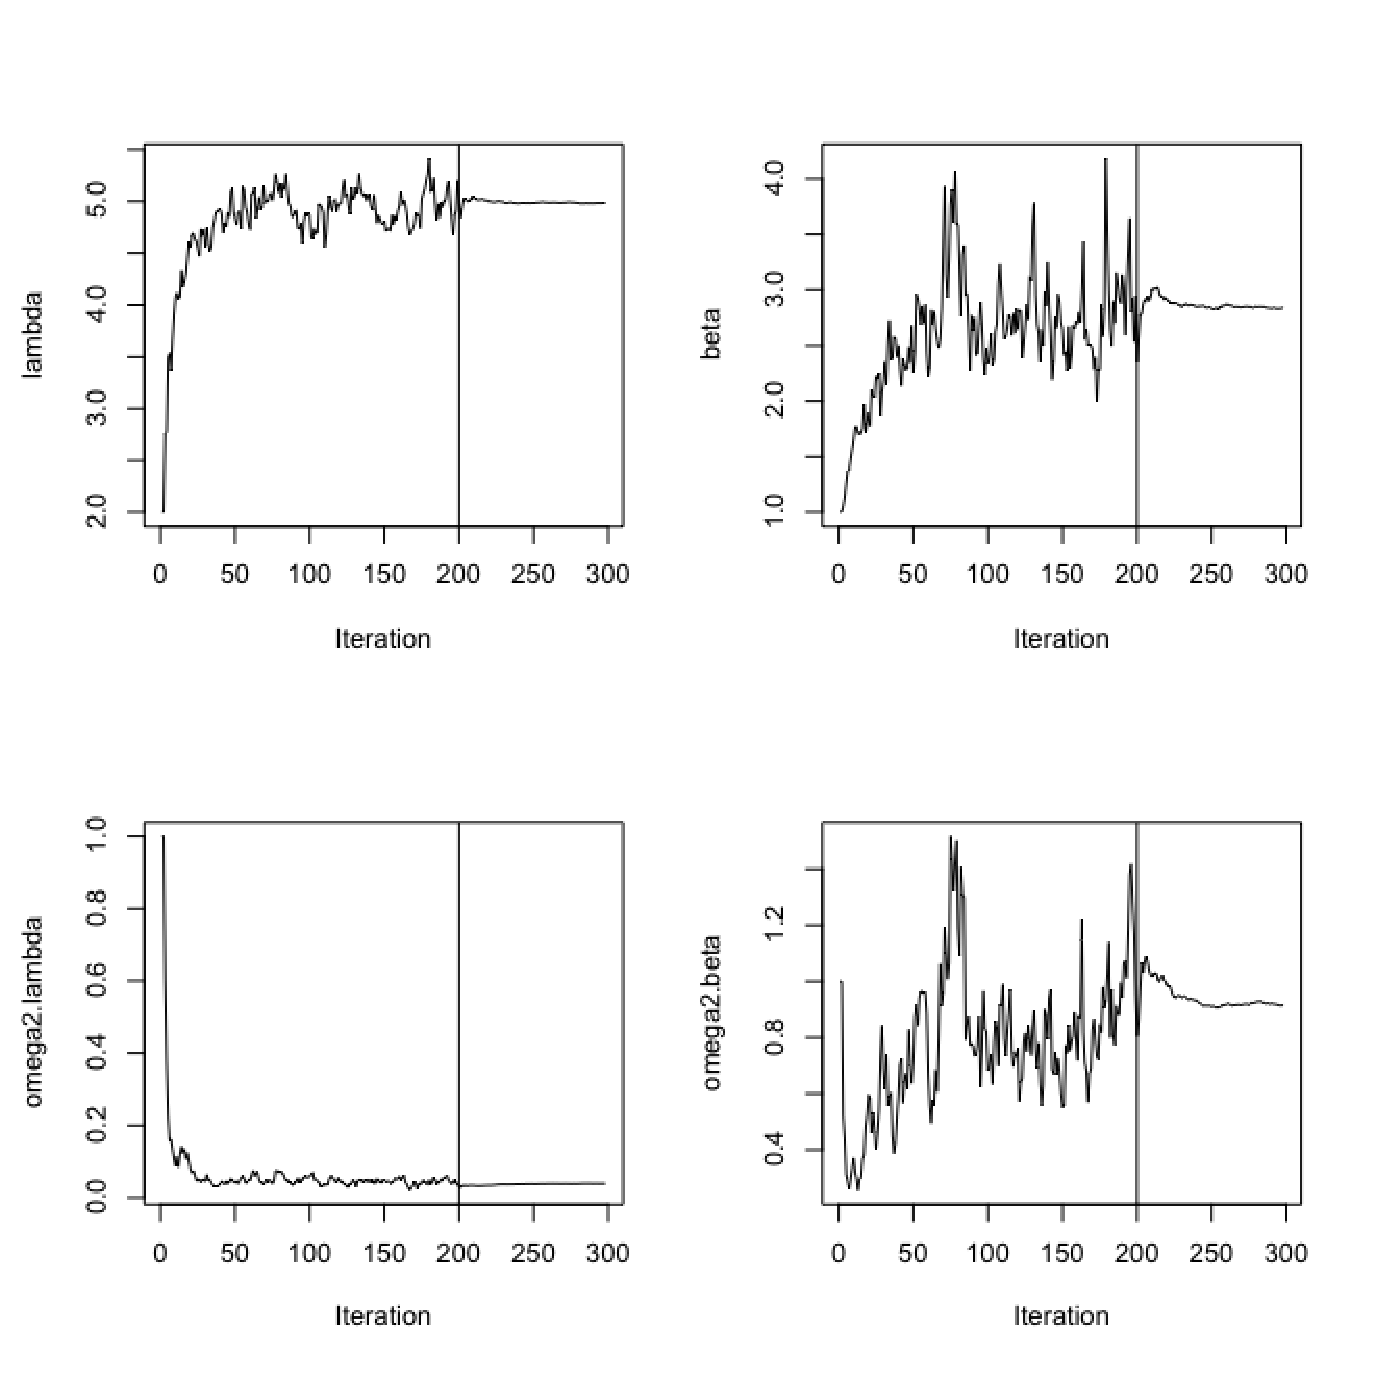
\epsfig{file=figs/popparam_tte.eps,width=9cm,angle=270}
\end{center}
\par \kern -0.5cm
\caption{Time-to-event data modelling: convergence of the empirical quantiles of order 0.1, 0.5 and 0.9 of $\dens(\psi_i | y_i ; \theta)$ for a single individual. The reference MH algorithm is in blue and the nlme-IMH is in red.} \label{fig:popTTE}
\end{figure}




\section{Discrete data}

\subsection{Binary data} \label{sec:toenail}

\monolix~3.0 can now be used to estimate the parameters of a model where the outcome is a discrete response. The most simple of this, but also the least informative type, is a binary response that can take the values 0 or 1. In this section, we illustrate the use of \monolix to model binary data from a randomised clinical trial comparing two treatments for fungal toenail infection. We use the {\sf toenail} dataset available in {\sf R} in the packages {\sf prLogistic} or {\sf HSAUR3}.

Data are from \cite{debacker_toenail}, a multi-center randomised comparison  of two oral treatments (A and B) for toenail infection. 294 patients are measured at seven visits, i.e. at baseline (week 0), and at weeks 4, 8, 12, 24, 36, and 48 thereafter, comprising a total of 1908 measurements. The primary end point was the absence of toenail infection and the outcome of interest is the binary variable "onycholysis" which indicates the degree of separation of the nail plate from the nail-bed (categorised as 0=none or mild versus 1=moderate or severe). Figure~\ref{fig:toenailData} shows the evolution of the number of events (left) and the proportion of events (right) in the two treatment groups over the 7 visits of the study.

\begin{figure}[!h]
\begin{center}
\epsfig{file=figs/toenail_barplotData.eps,width=7.5cm,angle=0}
\epsfig{file=figs/toenail_rawdata.eps,width=7.5cm,angle=0}
\end{center}
\par \kern -0.5cm
\caption{Toenail data. Left: number of events at each visit; right: proportion of infected subjects at each visit.} \label{fig:toenailData}
\end{figure}

Several analyses have been made in the literature \cite{lesaffre2001effect,lin2011goodness}, and here we fit the logistic random effect model developed by \cite{hedeker1994random}. This model includes a random intercept ($\theta_1$, normally distributed with a standard deviation $\omega_1$),  a time effect ($\beta_2$, normally distributed with a standard deviation $\omega_2$). Treatment (A or B) ($\beta$) is included as a covariate on time. The treatments were randomised at baseline so we don't include a treatment effect on the intercept. The probability $p_{ij}=P(Y_{ij}=1 | \theta_{1,i}, \theta_{2,i})$ associated with an event $Y_{ij}$ at time $t_{ij}$ is given by the following equation for the logit:
\begin{equation}
logit(p_{ij}) = \ln \left( \frac{p_{ij}}{1-p_{ij}} \right) = \theta_{1,i} + \theta_{1,i} t_{ij}
\end{equation}

For non-gaussian models, the model function must be written to return the log-pdf, that is, the logarithm of the probability of the observed response given a set of parameters. To do this we need to pass the response as one of the predictors.
\begin{verbatim}
data(toenail.saemix)
saemix.data<-saemixData(name.data=toe,name.group=c("id"),name.predictors=c("time","y"), 
    name.response="y", name.covariates=c("treatment"),name.X=c("time"))
\end{verbatim}

To tell \monolix~that we are now dealing with non-continuous responses, we add the argument {\sf modelType='likelihood'} to the definition of the model using the function {\sf saemixModel}. We assume only the intercept has interindividual variability, and follows a normal distribution. We set the covariate model for a treatment effect on $\theta_2$. 
\begin{verbatim}
binary.model<-function(psi,id,xidep) {
  tim<-xidep[,1]
  y<-xidep[,2]
  inter<-psi[id,1]
  slope<-psi[id,2]
  logit<-inter+slope*tim
  pevent<-exp(logit)/(1+exp(logit))
  pobs = (y==0)*(1-pevent)+(y==1)*pevent
  logpdf <- log(pobs)
  return(logpdf)
}

saemix.model<-saemixModel(model=binary.model,description="Binary model",
    modeltype="likelihood",
    psi0=matrix(c(-5,-.1,0,0),ncol=2,byrow=TRUE,dimnames=list(NULL,
    c("theta1","theta2"))),
    transform.par=c(0,0), covariate.model=c(0,1),
    covariance.model=matrix(c(1,0,0,1),ncol=2))
\end{verbatim}

We then fit the model, setting the option {\sf fim=FALSE} as the approximation used in the computation of the FIM by linearisation is not appropriate in discrete models. Since binary data contains very limited information, it is advised to increase the number of chains to stabilise the estimation. Here we set the number of chains to 10.
\begin{verbatim}
saemix.options<-list(seed=1234567,save=FALSE,save.graphs=FALSE, 
    displayProgress=FALSE, nb.chains=10, fim=FALSE)
binary.fit<-saemix(saemix.model,saemix.data,saemix.options)
\end{verbatim}

{\bf Important note:} The linear approximation of the FIM does not apply well to discrete response models. Exact computation methods to estimate the FIM without linearisation have been proposed by~\cite{Riviere16} using Hamiltonian Monte-Carlo and~\cite{Ueckert16} using adaptive Gaussian quadrature. These methods can be applied to estimate SE for the parameters but are not automatically available yet in \monolix.

\paragraph{Diagnostics:} automated visualisation or diagnostic plots have not yet been implemented for discrete response models, but we can of course create our own in R by simulating from the model. To to this we need to define a simulation function associated with the structural model, with the same arguments as the model function, and returning simulated responses. For the binary model, this function would be the following, where we replace the line defining the log-probability {\sf logp} in {\sf binary.model} with a line simulating from a Binomial distribution with parameter $pevent$ for each value of time, and returning those simulated events.
% ECO TODO: add Marc's npd for categorical data...

\begin{verbatim}
simulBinary<-function(psi,id,xidep) {
  tim<-xidep[,1]
  y<-xidep[,2]
  inter<-psi[id,1]
  slope<-psi[id,2]
  logit<-inter+slope*tim
  pevent<-1/(1+exp(-logit))
  ysim<-rbinom(length(tim),size=1, prob=pevent)
  return(ysim)
}
nsim<-100
binary.fit <- simulateDiscreteSaemix(binary.fit, simulBinary, nsim=nsim)
\end{verbatim}

In figure~\ref{fig:toenailPropVPC} we use the simulated data in the {\sf datasim} dataframe contained in the {\sf sim.data} element of the object after the call to the function to compute a 90\% prediction interval on the proportion of events at each visit. This VPC plot shows a reasonable model fit in the two treatment groups.

\begin{figure}[!h]
\begin{center}
\epsfig{file=figs/toenail_globalVPC.eps,width=11cm,angle=0}
\end{center}
\par \kern -0.5cm
\caption{Proportion of expected events compared to the observed proportion across time, for the model fit to the toenail data.} \label{fig:toenailPropVPC}
\end{figure}

The following code was used to produce this plot:
\begin{verbatim}
simdat <-binary.fit@sim.data@datasim
simdat$visit<-rep(toenail.saemix$visit,nsim)
simdat$treatment<-rep(toenail.saemix$treatment,nsim)
 
# requires 
# library(tidyverse)
# library(ggplot2)
# library(gridExtra)

ytab<-NULL
for(irep in 1:nsim) {
  xtab<-simdat[simdat$irep==irep,]
  xtab1 <- xtab %>%
    group_by(visit, treatment) %>%
    summarise(nev = sum(ysim), n=n()) %>%
    mutate(freq = nev/n)
  ytab<-rbind(ytab,xtab1[,c("visit","freq","treatment")])
}
gtab <- ytab %>%
  group_by(visit, treatment) %>%
  summarise(lower=quantile(freq, c(0.05)), median=quantile(freq, c(0.5)), 
  upper=quantile(freq, c(0.95))) %>%
  mutate(treatment=ifelse(treatment==1,"B","A"))
gtab$freq<-1

# summarising data
toe1 <- toenail.saemix %>%
  group_by(visit, treatment) %>%
  summarise(nev = sum(y), n=n()) %>%
  mutate(freq = nev/n, sd=sqrt((1-nev/n)/nev)) %>%
  mutate(treatment=ifelse(treatment==1,"B","A"))

plot2 <- ggplot(toe1, aes(x=visit, y=freq, group=treatment)) + 
  geom_line(aes(colour=treatment)) + 
  geom_point(aes(colour=treatment)) + 
  geom_line(data=gtab, aes(x=visit, y=median), linetype=2, colour='lightblue') + 
  geom_ribbon(data=gtab,aes(ymin=lower, ymax=upper), alpha=0.5, fill='lightblue') +
  ylim(c(0,0.5)) + theme_bw() + theme(legend.position = "none") + 
  facet_wrap(.~treatment) +
  xlab("Visit number") + ylab("Frequency of infection")
print(plot2)
\end{verbatim}


\clearpage
\newpage

\subsection{Categorical data} \label{sec:kneeCat}

The {\sf knee.saemix} data represents pain scores recorded in a clinical study in 127 patients with sport related injuries treated with two different therapies. The pain occuring during knee movement was observed after 3,7 and 10 days of treatment. It was taken from the {\sf catdata} package in R~\cite{catdata} (dataset {\sf knee}) and reformatted as follows. A time column was added representing the day of the measurement (with 0 being the baseline value) and each observation corresponds to a different line in the dataset. Treatment was recoded as 0/1 (placebo/treatment), gender as 0/1 (male/female) and {\sf Age2} represents the squared of centered Age. Figure~\ref{fig:kneeData} shows barplots of the different pain scores as a function of time in study, illustrating a recovery as the proportion of lower pain scores increases.

\begin{figure}[!h]
\begin{center}
\epsfig{file=figs/knee_barplotData.eps,width=11cm,angle=0}
\end{center}
\par \kern -0.5cm
\caption{Barplot of the evolution of pain scores with time in the {\sf knee.saemix} dataset.} \label{fig:kneeData}
\end{figure}

\begin{verbatim}
data(knee.saemix)
\end{verbatim}

The dataset is part of the datasets analysed in~\cite{Tutz12} with various methods (please refer to the different vignettes in the documentation of {\sf knee}), but mainly as logistic regression on the response after 10 days, or as mixed binary regression after dichotomising the response. Here, we will fit the following proportional odds model to the full data:
The probability $p_{ij}=P(Y_{ij}=1 | \theta_{1,i}, \theta_{2,i})$ associated with an event $Y_{ij}$ at time $t_{ij}$ is given by the following equation for the logit:
\begin{equation}
\begin{split}
logit(P(Y_{ij} = 1 | \psi_i)) &= \alpha_{1,i} + \beta_{i} t_{ij} \\
logit(P(Y_{ij} = 2 | \psi_i)) &= \alpha_{1,i} + \alpha_2 \\
logit(P(Y_{ij} = 3 | \psi_i)) &= \alpha_{1,i} + \alpha_2 + \alpha_3 \\
logit(P(Y_{ij} = 4 | \psi_i)) &= \alpha_{1,i} + \alpha_2 + \alpha_3 +\alpha_4\\
P(Y_{ij} = 4 | \psi_i) &= 1 - \sum_k=1^4 P(Y_{ij} = k | \psi_i)\\
\end{split}
\end{equation}
where $\alpha_1$ and $\beta$ have interindividual variability, $\beta$ is the effect of time, $\alpha_1$ is the probability of a pain score of 1 and the other parameters represent an incremental risk to move into the higher pain category.

When the response has more than one category, we define the probability for (K-1) categories and combine them to obtain the likelihood for each observation.

\begin{verbatim}
ordinal.model<-function(psi,id,xidep) {
  y<-xidep[,1]
  time<-xidep[,2]
  alp1<-psi[id,1]
  alp2<-psi[id,2]
  alp3<-psi[id,3]
  alp4<-psi[id,4]
  beta<-psi[id,5]
  
  logit1<-alp1 + beta*time
  logit2<-logit1+alp2
  logit3<-logit2+alp3
  logit4<-logit3+alp4
  pge1<-exp(logit1)/(1+exp(logit1))
  pge2<-exp(logit2)/(1+exp(logit2))
  pge3<-exp(logit3)/(1+exp(logit3))
  pge4<-exp(logit4)/(1+exp(logit4))
  pobs<-(y==1)*pge1+(y==2)*(pge2-pge1)+(y==3)*(pge3-pge2)+(y==4)*(pge4-pge3)+(y==5)*(1-pge4)
  logpdf <- log(pobs)  
  return(logpdf)
}  
saemix.model<-saemixModel(model=ordinal.model,
        description="Ordinal categorical model",modeltype="likelihood",
        psi0=matrix(c(0,0.2, 0.6, 3, 0.2),ncol=5,byrow=TRUE,
           dimnames=list(NULL,c("alp1","alp2","alp3","alp4","beta"))),
        transform.par=c(0,1,1,1,1),
        covariance.model = diag(c(1,0,0,0,1)))

saemix.options<-list(seed=632545,save=FALSE,save.graphs=FALSE, nb.chains=10, 
    fim=FALSE)

ord.fit<-saemix(saemix.model,saemix.data,saemix.options)
\end{verbatim}

Figure~\ref{fig:kneeMedScoreVPC}, representing a VPC of the mean value of pain score at each time point, stratified over treatment, shows some model misfit especially for treatment 0. This figure was produced using simulations from the fitted model as in the binary data examples using the simulation function below.
\begin{figure}[!h]
\begin{center}
\epsfig{file=figs/knee_medianScoreVPC.eps,width=11cm,angle=0}
\end{center}
\par \kern -0.5cm
\caption{VPC of the mean value of pain score in the model adjusted to the {\sf knee.saemix} dataset.} \label{fig:kneeMedScoreVPC}
\end{figure}

\begin{verbatim}
simulateOrdinal<-function(psi,id,xidep) {
  y<-xidep[,1]
  time<-xidep[,2]
  alp1<-psi[id,1]
  alp2<-psi[id,2]
  alp3<-psi[id,3]
  alp4<-psi[id,4]
  beta<-psi[id,5]
  
  logit1<-alp1 + beta*time
  logit2<-logit1+alp2
  logit3<-logit2+alp3
  logit4<-logit3+alp4
  pge1<-exp(logit1)/(1+exp(logit1))
  pge2<-exp(logit2)/(1+exp(logit2))
  pge3<-exp(logit3)/(1+exp(logit3))
  pge4<-exp(logit4)/(1+exp(logit4))
  x<-runif(length(time))
  ysim<-1+as.integer(x>pge1)+as.integer(x>pge2)+as.integer(x>pge3)+as.integer(x>pge4)
  return(ysim)
}
\end{verbatim}


\subsection{Count data} 

\subsubsection{Epilepsy data} \label{sec:epilepsyCount}

We first show a simple example using the {\sf epilepsy} data from the {\sf MASS} package. We can fit the Poisson model to the data, which assumes that the probability to observe a count value equal to $n$ is given by:
\begin{equation}
P(Y=n) = \frac{\lambda^n \; e^{-\lambda}}{n!}
\end{equation}

where $\lambda>0$ is the parameter of the model. We asssume a log-normal distribution for $\lambda$.

\begin{verbatim}
epilepsy<-MASS::epil
saemix.data<-saemixData(name.data=epilepsy, name.group=c("subject"),
     name.predictors=c("period","y"),name.response=c("y"),
     name.covariates=c("trt","base", "age"), 
     units=list(x="2-week",y="", covariates=c("","","yr")))
## Poisson model with one parameter
countPoi<-function(psi,id,xidep) { 
    y<-xidep[,2]
    lambda<-psi[id,1]
    logp <- -lambda + y*log(lambda) - log(factorial(y))
    return(logp)
    }
saemix.model<-saemixModel(model=countPoi,description="Count model Poisson",
   modeltype="likelihood", 
   psi0=matrix(c(0.5),ncol=1,byrow=TRUE,dimnames=list(NULL, c("lambda"))), 
   transform.par=c(1))
saemix.options<-list(seed=632545,save=FALSE,save.graphs=FALSE, 
   displayProgress=FALSE)
poisson.fit<-saemix(saemix.model,saemix.data,saemix.options)
\end{verbatim}


\subsubsection{RAPI data} \label{sec:RAPICount}

This dataset was kindly made available by David Atkins (University of Washington) in his tutorial on modelling count data~\cite{Atkins13}. The RAPI data studies gender differences across two years in alcohol-related problems, as measured by the Rutgers Alcohol Problem Index (RAPI)~\cite{White89}. Students were asked to report every six months the number of alcohol-related problems, and the dataset includes 3,616 repeated measures of these counts in 818 subjects, 561 of whom had the full 5 measurements over a period of 2 years. Interesting features of this dataset are first, the longitudinal aspect which allow to evaluate changes over time, and second, the shape of the distribution of counts. Counts are often positively skewed, bounded by zero, with a large stack of data points at zero, indicating individuals and/or occasions without drinking, use, or related problems. This dataset was used in~\cite{Atkins13} to illustrate mixed effects count regression using the {\sf glmer()} function from the {\sf lme4}.

The dataset is available in \monolix~under the name {\sf rapi.saemix} so we read it and create our saemixData object in the usual way. Because we need the value of the outcome to compute the corresponding likelihood, the {\sf rapi} column is used both as a predictor and as the response:
\begin{verbatim}
data(rapi.saemix)
saemix.data<-saemixData(name.data=rapi.saemix, name.group=c("id"),
                 name.predictors=c("time","rapi"),name.response=c("rapi"),
                 name.covariates=c("gender"),
                 units=list(x="months",y="",covariates=c("")))
hist(rapi.saemix$rapi, main="", xlab="RAPI score", breaks=30)
\end{verbatim}
\monolix~currently does not have automated plots for discrete outcome data, but we can produce our own histogram (here, across all measurements without taking time into account) to notice that indeed, there seems to be many subjects reporting no alcohol related problems over some periods.

\paragraph{Poisson model:} the first model we can fit to this data is, as previously, the Poisson model, but this time we add a time effect. Here we will write the same model as in {\sf glmer()} to compare our results. In {\sf glmer()} a logarithmic link function is used to transform the mean of the Poisson model ($\lambda$) into a linear predictor of time and covariates. Random effects are then added to the parameters of the linear model. To take into account the change with time in {\sf saemix}, we need to rewrite the previous model to use normal distributions for the parameters and explicitely write the linear model in the function, as follows:
\begin{verbatim}
count.poisson<-function(psi,id,xidep) { 
  time<-xidep[,1]
  y<-xidep[,2]
  intercept<-psi[id,1]
  slope<-psi[id,2]
  lambda<- exp(intercept + slope*time)
  logp <- -lambda + y*log(lambda) - log(factorial(y))
  return(logp)
}
\end{verbatim}
The expression of logp in the model function is unchanged, but now we define a log-normal distribution for $\lambda$ within the model so that we can use two parameters and time as a predictor. The statistical model also changes to reflect this, as our parameters intercept and slope are now on the scale of the random effects, so they are given a normal distribution. Defining and fitting this model in \monolix, we have:
\begin{verbatim}
saemix.model.poi<-saemixModel(model=count.poisson,description="Count model Poisson",
    modeltype="likelihood",   
    psi0=matrix(c(log(5),0.01),ncol=2,byrow=TRUE,dimnames=list(NULL, c("intercept","slope"))), 
    transform.par=c(0,0), omega.init=diag(c(0.5, 0.5)))
saemix.options<-list(seed=632545,save=FALSE,save.graphs=FALSE, displayProgress=FALSE)
poisson.fit<-saemix(saemix.model.poi,saemix.data,saemix.options)
\end{verbatim}
Note that when parameters enter the model through a normal distribution, we may need to adjust the initial values of the $\Omega$ matrix (argument {\sf omega.init}) to avoid failure to find valid initial parameter estimates.

We can also add the covariate gender to both parameters as well as a correlation between the two random effects:
\begin{verbatim}
modsmx.poi.cov2<-saemixModel(model=count.poisson,
      description="Count model Poisson",modeltype="likelihood",   
      psi0=matrix(c(log(5),0.01),ncol=2,byrow=TRUE,dimnames=list(NULL, 
      c("intercept","slope"))), transform.par=c(0,0), 
      omega.init=diag(c(0.5, 0.5)), 
      covariance.model=matrix(data=1, ncol=2, nrow=2),
      covariate.model=matrix(c(1,1), ncol=2, byrow=TRUE))
poisson.fit.cov2<-saemix(modsmx.poi.cov2,saemix.data,saemix.options)
\end{verbatim}
Comparing the parameter estimates from this fit to the estimates obtained by {\sf glmer()} using a Laplace approximation in Table~2 of~\cite{Atkins13}, we find very good agreement with the SAEM algorithm.

\noindent{\bf Note:} \monolix~does not provide adequate standard errors of estimation for the parameters in version 3.0. The FO-approximation of the FIM implemented in the current version of the algorithm is known to be very poor for discrete outcome models.

Some diagnostics for this model can be obtained by simulating from the model. To to this we need to define a simulation function associated with the structural model, with the same arguments as the model function, and returning simulated responses. For the Poisson model, this function would be the following, where we replace the line defining the log-probability {\sf logp} in {\sf count.poisson} with a line simulating from a Poisson distribution with parameter $\lambda$ for each value of time, and returning those simulated counts.
\begin{verbatim}
saemix.simulatePoisson<-function(psi, id, xidep) {
  time<-xidep[,1]
  y<-xidep[,2]
  intercept<-psi[id,1]
  slope<-psi[id,2]
  lambda<- exp(intercept + slope*time)
  y<-rpois(length(time), lambda=lambda)
  return(y)
}
\end{verbatim}

We then use the {\sf simulateDiscreteSaemix} function to obtain simulations from the model, using the estimated parameters. Here we set the number of simulations to 100 as the dataset is large and we are interested in global diagnostics.
\begin{verbatim}
yfit1<-simulateDiscreteSaemix(poisson.fit.cov2, simulate.function=saemix.simulatePoisson, 
    nsim=100)
cat("Observed proportion of 0's", 
     length(yfit1@data@data$rapi[yfit1@data@data$rapi==0])/yfit1@data@ntot.obs,"\n")
cat("      Poisson model, p=",
    length(yfit1@sim.data@datasim$ysim[yfit1@sim.data@datasim$ysim==0])/
    length(yfit1@sim.data@datasim$ysim),"\n") 
\end{verbatim}

\paragraph{Handling overdispersion:} the model predicts a lower proportion of subjects without alcohol-related problems than we observe in data, a sign of overdispersion (with a Poisson model, the mean of the Poisson distribution, $\lambda$, is equal to the variance, an assumption which is violated here). Several models can be used to take this feature into account. First, we can use the Zero-Inflated Poisson model, where the number of counts equal to 0 is increased. This model can be built as a mixture between a distribution of 0's with probability $p_0$ and a standard Poisson model. We modify our model function above to:
\begin{verbatim}
count.poissonzip<-function(psi,id,xidep) {
  time<-xidep[,1]
  y<-xidep[,2]
  intercept<-psi[id,1]
  slope<-psi[id,2]
  p0<-psi[id,3] # Probability of zero's
  lambda<- exp(intercept + slope*time)
  logp <- log(1-p0) -lambda + y*log(lambda) - log(factorial(y)) # Poisson
  logp0 <- log(p0+(1-p0)*exp(-lambda)) # Zeroes
  logp[y==0]<-logp0[y==0]
  return(logp)
}
\end{verbatim}
and fit the model using:
\begin{verbatim}
modsmx.zip<-saemixModel(model=count.poissonzip,description="count model ZIP",
   modeltype="likelihood", 
   psi0=matrix(c(1.5, 0.01, 0.2),ncol=3,byrow=TRUE,dimnames=list(NULL, 
      c("intercept", "slope","p0"))), 
   transform.par=c(0,0,3), covariance.model=diag(c(1,1,0)), 
   omega.init=diag(c(0.5,0.3,0)),
   covariate.model = matrix(c(1,1,0),ncol=3, byrow=TRUE))

zippoisson.fit <- saemix(modsmx.zip,saemix.data,saemix.options)
\end{verbatim}
where we assume a logit-normal distribution for the added parameter p0 through the transform.par argument. We could also model logit(p0) on a normal scale if we needed to add a time effect. The same approach as above can then be used to simulate from the model, this time using the simulation function:
\begin{verbatim}
saemix.simulatePoissonZIP<-function(psi, id, xidep) {
  time<-xidep[,1]
  y<-xidep[,2]
  intercept<-psi[id,1]
  slope<-psi[id,2]
  p0<-psi[id,3] # Probability of zero's
  lambda<- exp(intercept + slope*time)
  prob0<-rbinom(length(time), size=1, prob=p0)
  y<-rpois(length(time), lambda=lambda)
  y[prob0==1]<-0
  return(y)
}
\end{verbatim}
and we can check that the proportion of simulated 0's is now closer to the observed value.

A second type of model used in~\cite{Atkins13} is the hurdle model, which combines a binary logistic model for the probability of having counts greater than 0, with a truncated Poisson model for counts greater than 0. To implement this, we fit separately the two models: the binary logistic model is fit to the data where we use as a response the binary outcome with values 0 for counts of 0 and 1 for counts strictly positive, then the Poisson model is fit to the data excluding zero counts.

Other possible models include the negative binomial model and generalised Poisson models with additional parameters handling the overdispersion.

\paragraph{Diagnostics:} the simulation functions can be used to produce diagnostic plots. As an example, we can compare the expected proportion of 0's, representing subjects without alcohol problems, versus time and stratified by gender, to compare the different models (the code available as a notebook on the github for saemix). The results, shown in Figure~\ref{fig:rapiCompareProp0}. We could also look at the counts for different categories or the evolution of the median counts. 

\begin{figure}[!h]
\begin{center}
\epsfig{file=figs/rapi_comparePropNoDrinking.eps,width=14cm,angle=0}
\end{center}
\par \kern -0.5cm
\caption{Proportion of subjects without drinking problems versus time, for men and women, observed and expected for the Poisson, ZIP and hurdle models, for the RAPI data.} \label{fig:rapiCompareProp0}
\end{figure}


\section{Time-to-event data}

\subsection{Single event} \label{sec:lungtte}

The example chosen to illustrate the analysis of time-to-event data is the NCCTG Lung Cancer Data, describing the survival in patients with advanced lung cancer from the North Central Cancer Treatment Group~\cite{Loprinzi94}. Covariates measured in the study include performance scores rating how well the patient can perform usual daily activities. We reformatted the {\sf cancer} dataset provided in the {\sf survival} package in R~\cite{survivalPkg} in SAEM format: patients with missing age, sex, institution or physician assessments were removed from the dataset. Status was recoded as 1 for death and 0 for a censored event, and a censoring column was added to denote whether the patient was dead or alive at the time of the last observation. A line at time=0 was added for all subjects. Finally, subjects were numbered consecutively from 0 to 1.

We can use a Weibull model for the hazard, parameterised as $\lambda$ and $\beta$. For individual $i$, the hazard function of this model is:
\begin{align}\label{weibullmodel}
& h(t, \psi_i) = \frac{\beta_i}{\lambda_i}\left(\frac{t}{\lambda_i}\right)^{\beta_i-1}\eqs.
\end{align}
Here, the vector of individual parameters is $\psi_i = (\lambda_i, \beta_i)$. These two parameters are assumed to be independent and  lognormally distributed:
\begin{align} \label{indivtte}
& \log(\lambda_i) \sim \mathcal{N}(\log(\lambda_{\rm pop}), \omega^2_{\lambda})\eqs,\\
& \log(\beta_i) \sim \mathcal{N}(\log(\beta_{\rm pop}), \omega^2_{\beta})\eqs.
\end{align}
Then, the vector of population parameters is $\theta = (\lambda_{\rm pop}, \beta_{\rm pop}, \omega_{\lambda}, \omega_{\beta})$.

The survival function for this model is:
$$ S(t) = e^{ - \left( \frac{t}{\lambda} \right) ^{\beta}}$$

The model function for \monolix~needs to define the log-pdf for each observation. At time 0, it is 0 (no event has occurred yet). For a censored event, the log-likelihood is equal to the logarithm of the survival function since the beginning of the observation period, while for an observed event we add the logarithm of the hazard at the time of the event. In the model below, we pass individual censoring times as the third predictor, so that each individual may have his or her own follow-up duration.

\begin{verbatim}
weibulltte.model<-function(psi,id,xidep) {
  T<-xidep[,1]
  y<-xidep[,2] # events (1=event, 0=no event)
  cens<-which(xidep[,3]==1) # censoring times (subject specific)
  init <- which(T==0)
  lambda <- psi[id,1] # Parameters of the Weibull model
  beta <- psi[id,2]
  Nj <- length(T)
  
  ind <- setdiff(1:Nj, append(init,cens)) # indices of events
  hazard <- (beta/lambda)*(T/lambda)^(beta-1) # H'
  H <- (T/lambda)^beta # H
  logpdf <- rep(0,Nj) # ln(l(T=0))=0
  logpdf[cens] <- -H[cens] + H[cens-1] # ln(l(T=censoring time))
  logpdf[ind] <- -H[ind] + H[ind-1] + log(hazard[ind]) # ln(l(T=event time))
  return(logpdf)
}
\end{verbatim}


{\bf Important note:} In TTE models with a single event, there is not enough information to estimate interindividual variability, but \monolix~needs at least one parameter to run. In this case, we include a random effect in the model but it cannot be estimated properly.


\paragraph{Diagnostics:} Automated visualisation or diagnostic plots have not yet been implemented for discrete response models, but we can of course create our own in R. In Figure~\ref{fig:lungcompareKM} we used the linear approximation of the FIM and the delta-method to compute a very rough estimate of the confidence interval on the predicted survival curve, overlaying it to the non-parametric Kaplan-Meier estimate provided by the {\sf survival} package. Here despite its shortcomings the FIM approximation seems to be adequate.

\begin{figure}[!h]
\begin{center}
\epsfig{file=figs/lung_compareKM.eps,width=12cm,angle=270}
\end{center}
\par \kern -0.5cm
\caption{Survival function, as a Kaplan-Meier estimate (black) and fitted by a Weibull model with {\sf saemix} (red).} \label{fig:compareKM}
\end{figure}

We can also use simulations to compute the normalised prediction discrepancies (npd) developed by~\cite{Cerou18}.

\subsection{Repeated time-to-event}

For repeated time-to-event data, we use the same model function as above, as the likelihood of an event will be defined relative to the previous event until censoring occurs.

Repeated events were generated using simulx (mlxR package in R), for $N=100$ individuals, using the Weibull model \eqref{weibullmodel} with $\lambda_{\rm pop} = 10$, $\omega_{\lambda} = 0.3$, $\beta_{\rm pop} = 3$ and $\omega_{\beta} = 0.3$ and assuming a right censoring time $\tau_c = 20$.

The following code was used in R to run this example:

\begin{verbatim}
data(tte.saemix)
saemix.data<-saemixData(name.data=tte.saemix,header=TRUE,sep=" ",na=NA,
   name.group=c("id"),name.response=c("y"),name.predictors=c("time","y"), name.X=c("time"))

timetoevent.model<-function(psi,id,xidep) {
T<-xidep[,1]
N <- nrow(psi)
Nj <- length(T)
censoringtime = 20
lambda <- psi[id,1]
beta <- psi[id,2]
init <- which(T==0)
cens <- which(T==censoringtime)
ind <- setdiff(1:Nj, append(init,cens))
hazard <- (beta/lambda)*(T/lambda)^(beta-1)
H <- (T/lambda)^beta
logpdf <- rep(0,Nj)
logpdf[cens] <- -H[cens] + H[cens-1]
logpdf[ind] <- -H[ind] + H[ind-1] + log(hazard[ind])
return(logpdf)
}

saemix.model<-saemixModel(model=timetoevent.model,description="time model",
   type="likelihood",
   psi0=matrix(c(2,1),ncol=2,byrow=TRUE,dimnames=list(NULL,c("lambda","beta"))),
   transform.par=c(1,1),covariance.model=matrix(c(1,0,0,1),ncol=2,byrow=TRUE))

saemix.options<-list(map=F,fim=F,ll.is=F, nb.chains = 1, nbiter.saemix =c(200,100), displayProgress=TRUE,save.graphs=FALSE)

saemix.fit<-saemix(model,saemix.data,saemix.options)

\end{verbatim}

Figure \ref{fig:popTTE} shows the convergence of the population parameters for this example. The results are summarised in the following table:

\begin{verbatim}
----------------------------------------------------
----                  Results                   ----
----------------------------------------------------
-----------------  Fixed effects  ------------------
----------------------------------------------------
     Parameter Estimate
[1,] lambda    5.0     
[2,] beta      2.8     
----------------------------------------------------
-----------  Variance of random effects  -----------
----------------------------------------------------
       Parameter     Estimate
lambda omega2.lambda 0.039   
beta   omega2.beta   0.921   
----------------------------------------------------
------  Correlation matrix of random effects  ------
----------------------------------------------------
              omega2.lambda omega2.beta
omega2.lambda 1             0          
omega2.beta   0             1 
\end{verbatim}


\begin{figure}[!h]
\begin{center}
\par \kern -1cm
%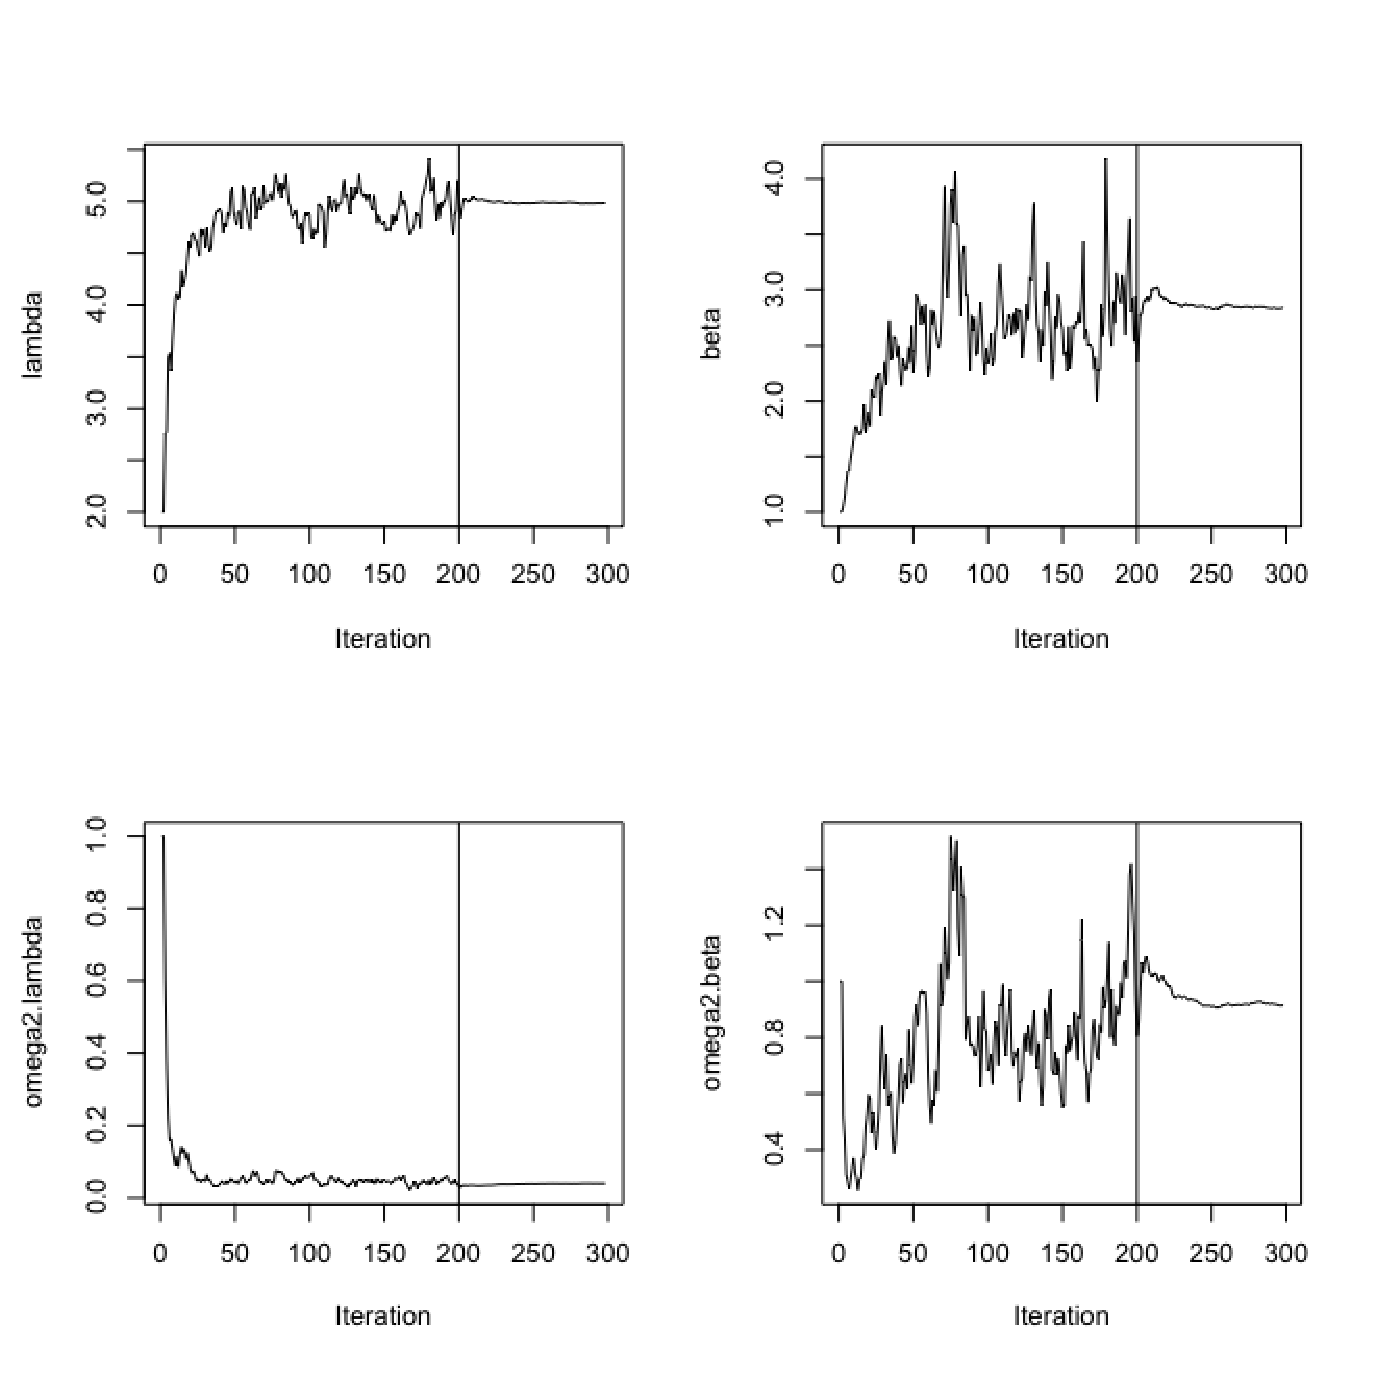
\epsfig{file=figs/popparam_tte.eps,width=12cm,angle=0}
\end{center}
\par \kern -0.5cm
\caption{Convergence plot obtained for the RTTE data} \label{fig:popTTE}
\end{figure}




\newpage
\addcontentsline{toc}{chapter}{{\bf Bibliography}}

\bibliography{docsaem}

\end{document}

